%https://github.com/SublimeText/LaTeXTools/issues/1439
%!TEX output_directory=latexcache

% You can build this using the command:
% latexmk -pdf -jobname=output -output-directory=cache -aux-directory=cache -pdflatex="pdflatex -interaction=nonstopmode" -use-make main.tex

% When the bibliography includes a cyclic reference to another bibliography,
% you need to run `pdflatex` 5 times on the following order:
% 1. `pdflatex`,
% 2. `biber`,
% 3. `pdflatex`
% 4. `pdflatex`
% 5. `pdflatex`
% 6. `biber`
% 7. `pdflatex`

% Monograph LaTeX Template for UFSC based on:
% 1. https://github.com/royertiago/tcc
% 2. http://portal.bu.ufsc.br/normalizacao/
% 3. https://github.com/evandrocoan/ufscthesisx
% 4. http://www.latextemplates.com/template/simple-sectioned-essay

% Initially translated from Portuguese with help of https://github.com/omegat-org/omegat <Computer Assisted Translation of LaTeX document>
% https://tex.stackexchange.com/questions/313732/computer-assisted-translation-of-latex-document

% Allows you to write your thesis both in English and Portuguese
% https://tex.stackexchange.com/questions/5076/is-it-possible-to-keep-my-translation-together-with-original-text
\newif\ifenglish\englishfalse
\newif\ifadvisor\advisorfalse

% Uncomment the line `\englishtrue` to set the document default language to English
% \englishtrue
\advisortrue

% https://tex.stackexchange.com/questions/131002/how-to-expand-ifthenelse-so-that-it-can-be-used-in-parshape
\newcommand{\lang}[2]{\ifenglish#1\else#2\fi}
\newcommand{\advisor}[2]{\ifadvisor#1\else#2\fi}

% https://tex.stackexchange.com/questions/385895/how-to-make-passoptionstopackage-add-the-option-as-the-last
% https://tex.stackexchange.com/questions/484400/changing-the-cleveref-package-language-conjunction-definition
% https://tex.stackexchange.com/questions/516058/why-isnt-my-biblatex-language-changing-when-passing-the-language-on-my-document
\ifenglish
    \PassOptionsToPackage{brazil,main=english,spanish,french}{babel}
\else
    \PassOptionsToPackage{main=brazil,english,spanish,french}{babel}
\fi

% Simple alias for English and Portuguese words
% https://tex.stackexchange.com/questions/513019/argument-of-bbltempd-has-an-extra
\newcommand{\brazilword}[1]{\protect\foreignlanguage{brazil}{#1}}
\newcommand{\englishword}[1]{\protect\foreignlanguage{english}{#1}}

% Allow you to write `Evandro's house` in latex as `Evandro\s house` instead of `Evandro\textquotesingle{}s house`
% https://tex.stackexchange.com/questions/31091/space-after-latex-commands
\newcommand{\s}[0]{\textquotesingle{}s\xspace}
\newcommand{\q}[0]{\textquotesingle{}\xspace}

% Uncomment the following line if you want to use other biblatex settings
% \PassOptionsToPackage{style=numeric,repeatfields=true,backend=biber,backref=true,citecounter=true}{biblatex}
\documentclass[
\lang{english}{brazilian,brazil}, % https://tex.stackexchange.com/questions/484400/changing-the-cleveref-package-language-conjunction-definition
12pt, % Padrão UFSC para versão final
a4paper, % Padrão UFSC para versão final
oneside, % Impressão nos dois lados da folha
chapter=TITLE, % Título de capítulos em caixa alta
section=TITLE, % Título de seções em caixa alta
]{setup/ufscthesisx}

% Utilize o arquivo aftertext/references.bib para incluir sua bibliografia.
% http://tug.ctan.org/tex-archive/macros/latex/contrib/cleveref/cleveref.pdf
\addbibresource{aftertext/references.bib}

% https://www.overleaf.com/learn/latex/Inserting_Images
\graphicspath{{pictures/}}

% FIXME: Preencha com seus dados
\autor{\brazilword{Gian Augusto Ortiz}}
\titulo{\lang{Work Title\protect\\Could be break into two lines}{Implementação de um Serviço de Checkpoint para arquitetura de Checkpoint/Restore de Stateful Containers no Kubernetes}}

% FIXME: Se houver subtítulo, descomente a linha abaixo
% \subtitulo{\lang{Subtitle}{Subtítulo}}

% FIXME: Siglas para grau de formação Dr./Dra., Me./Ma, Bel. Bela. (inglês: PhD., MSc., Bs.)
\orientador[\lang{Supervisor}{Orientador}]{\brazilword{Odorico Machado Mendizabal}, \lang{Phd.}{Dr.}}

% FIXME: Se houver coorientador, descomente a linha abaixo
% \coorientador[\lang{Co-supervisor}{Coorientador(a)}]{\brazilword{Nome do coorientador(a)}, \lang{Phd.}{Dr.}}

% FIXME: Preencher com o nome do Coordenador de TCCs/Teses do seu curso
\coordenador[\lang{Coordinator}{Coordenador}]{\brazilword{Lúcia Helena Martins Pacheco}, \lang{Phd.}{Dr.}}

% FIXME: Local da sua defesa
\local{\brazilword{Florianópolis, Santa Catarina} -- \lang{Brazil}{Brasil}}

% FIXME: Ano da sua defesa
\ano{2023}
\biblioteca{\lang{University Library}{Biblioteca Universitária}}

% FIXME: Sigla da sua instituição
\instituicaosigla{UFSC}
\instituicao{\brazilword{Universidade Federal de Santa Catarina}}

% FIXME: Preencha com Tese, Dissertação, Monografia ou Trabalho de Conclusão de Curso, Bachelor's Thesis, etc
\tipotrabalho{\lang{Bachelor\s Thesis}{Trabalho de Conclusão de Curso}}

% FIXME: Se houver Área de Concentração, descomente a linha abaixo
% \area{\lang{Formal Languages}{Linguagens Formais}}

% FIXME: Preencha com Doutor, Bacharel ou Mestrando
\formacao{\lang
    {Bachelor of Science degree in Computer Science}
    {Bacharel em Ciências da Computação}%
}
\programa{\lang
    {Undergraduate Program in Computer Science}
    {Programa de Graduação em Ciências da Computação}%
}

% FIXME: Preencha com Departamento de XXXXXX, Centro de XXXXXX
\centro{\lang
    {INE -- Department of Informatics and Statistics, CTC -- Technological Center}
    {INE -- Departamento de Informática e Estatística, CTC -- Centro Tecnológico}%
}

% FIXME: Preencha com Campus XXXXXX     ou     Centro de XXXXXX
\campus{\brazilword{Campus Reitor João David Ferreira Lima}}

% FIXME: Data da sua defesa
\data{\lang{13 of november of}{13 de novembro de} 2023}

% O preambulo deve conter tipo do trabalho, objetivo, nome da instituição e a área de concentração.
\preambulo{\lang%
    {%
        \imprimirtipotrabalho~submitted to the \imprimirprograma~of
        \imprimirinstituicao~for degree acquirement in \imprimirformacao.%
    }{%
        \imprimirtipotrabalho~submetido ao \imprimirprograma~da
        \imprimirinstituicao~para a obtenção do Grau de \imprimirformacao.%
    }%
}

% Allows you to use ~= instead of `\hyp{}`
% https://tex.stackexchange.com/questions/488008/how-to-create-an-alternative-to-shortcut-or-hyp
% https://tex.stackexchange.com/questions/405718/depending-on-babel-language-setting-i-get-biblatex-error-argument-of-language
% https://tex.stackexchange.com/questions/340661/argument-of-languageactivearg-has-an-extra-i-use-includegraphics-and-r
\useshorthands{~}\defineshorthand{~=}{\hyp{}}

\palavraschaveufsc{palavraschaveingles}   {Checkpoint/Restore}
\palavraschaveufsc{palavraschaveportugues}{Checkpoint/Restore}

\palavraschaveufsc{palavraschaveingles}   {Stateful Container}
\palavraschaveufsc{palavraschaveportugues}{Conteiner Stateful}

\palavraschaveufsc{palavraschaveingles}   {Kubernetes}
\palavraschaveufsc{palavraschaveportugues}{Kubernetes}

\palavraschaveufsc{palavraschaveingles}   {Event Sourcing}
\palavraschaveufsc{palavraschaveportugues}{Event Sourcing}

\palavraschaveufsc{palavraschaveingles}   {Fault tolerance}
\palavraschaveufsc{palavraschaveportugues}{Tolerância a falhas}

\hypersetup
{
    pdfsubject={Thesis' Abstract},
    pdfcreator={LaTeX with abnTeX2 for UFSC},
    pdftitle={\imprimirtitulo},
    pdfauthor={\imprimirautor},
    pdfkeywords={\lang{\palavraschaveinglessemitem}{\palavraschaveportuguessemitem}},
}

% Altere o arquivo 'settings.tex' para incluir customizações de aparência da sua tese
%----------------------------------------------------------------------------------------
%   Thesis Tweaks and Utilities
%----------------------------------------------------------------------------------------
\makeatletter


% Uncomment this if you are debugging pages' badness Underfull & Overflow
% https://tex.stackexchange.com/questions/115908/geometry-showframe-landscape
% https://tex.stackexchange.com/questions/387077/what-is-the-difference-between-usepackageshowframe-and-usepackageshowframe
% https://tex.stackexchange.com/questions/387257/how-to-do-the-memoir-headings-fix-but-not-have-my-text-going-over-the-page-botto
% https://tex.stackexchange.com/questions/14508/print-page-margins-of-a-document
% \usepackage[showframe,pass]{geometry}

% To use the font Times New Roman, instead of the default LaTeX font
% more up-to-date than '\usepackage{mathptmx}'
% \usepackage{newtxtext}
% \usepackage{newtxmath}

% https://tex.stackexchange.com/questions/182569/how-to-manually-set-where-a-word-is-split
\hyphenation{Ge-la-im}
\hyphenation{Cis-la-ghi}

% Add missing translations for Portuguese
% https://tex.stackexchange.com/questions/8564/what-is-the-right-way-to-redefine-macros-defined-by-babel
\@ifpackageloaded{babel}{\@ifpackagewith{babel}{brazil}{\addto\captionsbrazil{%
  \renewcommand{\mytextpreliminarylistname}{Breve Sumário}
}}{}}{}
\@ifundefined{advisor}{\newcommand{\advisor}[2]{#1}}{}

% Selects a sans serif font family
% \renewcommand{\sfdefault}{cmss}

% Selects a monospaced (“typewriter”) font family
% \renewcommand{\ttdefault}{cmtt}

% Spacing between lines and paragraphs
% https://tex.stackexchange.com/questions/70212/ifpackageloaded-question
\@ifclassloaded{memoir}
{
  % New custom chapter style VZ14, see other chapters styles in:
  % http://repositorios.cpai.unb.br/ctan/info/latex-samples/MemoirChapStyles/MemoirChapStyles.pdf
  \newcommand\thickhrulefill{\leavevmode \leaders \hrule height 1ex \hfill \kern \z@}
  \makechapterstyle{VZ14} { %
    % \thispagestyle{empty}
    \setlength\beforechapskip{50pt}
    \setlength\midchapskip{20pt}
    \setlength\afterchapskip{20pt}
    \renewcommand\chapternamenum{}
    \renewcommand\printchaptername{}
    \renewcommand\chapnamefont{\Huge\scshape}
    \renewcommand\printchapternum {%
      \chapnamefont\null\thickhrulefill\quad
      \@chapapp\space\thechapter\quad\thickhrulefill
    }
    \renewcommand\printchapternonum {%
      \par\thickhrulefill\par\vskip\midchapskip
      \hrule\vskip\midchapskip
    }
    \renewcommand\chaptitlefont{\huge\scshape\centering}
    \renewcommand\afterchapternum {%
      \par\nobreak\vskip\midchapskip\hrule\vskip\midchapskip
    }
    \renewcommand\afterchaptertitle {%
      \par\vskip\midchapskip\hrule\nobreak\vskip\afterchapskip
    }
  }

  % Apply the style `VZ14` just created
  % \chapterstyle{VZ14}

  % http://mirrors.ibiblio.org/CTAN/macros/latex/contrib/memoir/memman.pdf
  \setlength\beforechapskip{0pt}
  \setlength\midchapskip{15pt}
  \setlength\afterchapskip{15pt}

  % Memoir: Warnings “The material used in the headers is too large” w/ accented titles
  % https://tex.stackexchange.com/questions/387293/how-to-change-the-page-layout-with-memoir
  \setheadfoot{30.0pt}{\footskip}
  \checkandfixthelayout
}{}

% Controlling the spacing between one paragraph and another
% Default value for UFSC 0.0cm
\setlength{\parskip}{\advisor{0.0cm}{0.2cm}}

% Paragraph size is given by
% Default value for UFSC 1.5cm
% \setlength{\parindent}{1.3cm}

% https://tex.stackexchange.com/questions/148647/how-to-remove-space-before-enumerate
% https://tex.stackexchange.com/questions/433543/behaviour-of-enumitem-setlist
\advisor{}{
    \setlist*[enumerate]{label=\arabic*,}
    \setlist*[enumerateoptional]{label=\arabic*,}

    % https://tex.stackexchange.com/questions/24454/space-after-float-with-h
    % https://tex.stackexchange.com/questions/23313/how-can-i-reduce-padding-after-figure
    \AtBeginEnvironment{figure}{
      \setlength{\intextsep}{5pt} % Vertical space above & below [h] floats
      % \setlength{\textfloatsep}{10pt} % Vertical space below (above) [t] ([b]) floats
      % \setlength{\abovecaptionskip}{10pt}
      % \setlength{\belowcaptionskip}{5pt}
    }

    % Patch the `abntex2` citacao environment removing the extra space from its top
    % https://tex.stackexchange.com/questions/300340/topsep-itemsep-partopsep-and-parsep-what-does-each-of-them-mean-and-wha
    \xpatchcmd{\citacao}
    {\list{}}
    {\list{}{\topsep=0pt}}
    {}
    {\FAILEDPATCHINGCITACAO}
}


% Color settings across the document
\@ifpackageloaded{xcolor}
{
  % RGB colors in absolute values from 0 to 255 by using `RGB` tag
  \definecolor{darkblue}{RGB}{26,13,178}

  % Colors names definitions as RGB colors in percentage notation by using `rgb` tag
  \definecolor{mygreen}{rgb}{0,0.6,0}
  \definecolor{mygray}{rgb}{0.5,0.5,0.5}
  \definecolor{mymauve}{rgb}{0.58,0,0.82}
  \definecolor{figcolor}{rgb}{1,0.4,0}
  \definecolor{tabcolor}{rgb}{1,0.4,0}
  \definecolor{eqncolor}{rgb}{1,0.4,0}
  \definecolor{linkcolor}{rgb}{1,0.4,0}
  \definecolor{citecolor}{rgb}{1,0.4,0}
  \definecolor{seccolor}{rgb}{0,0,1}
  \definecolor{abscolor}{rgb}{0,0,1}
  \definecolor{titlecolor}{rgb}{0,0,1}
  \definecolor{biocolor}{rgb}{0,0,1}
  \definecolor{blue}{RGB}{41,5,195}

  % PDF Hyperlinks settings
  \@ifpackageloaded{hyperref}
  {
    \hypersetup
    {
      colorlinks=true,     % false: boxed links; true: colored links
      linkcolor=darkblue,  % color of internal links
      citecolor=darkblue, % color of links to bibliography
      filecolor=black,     % color of file links
      urlcolor=\advisor{black}{darkgreen},
      bookmarksdepth=4,
      pdfencoding=auto,%
      psdextra,
    }
  }
}{}


% Filtering and Mapping Bibliographies
% \DeclareFieldFormat{url}{Disponível~em:\addspace\url{#1}}

% https://tex.stackexchange.com/questions/517526/how-to-make-biblatex-url-links-generated-with-brackets-around-it-url-correctly
\DeclareFieldFormat{url}{\bibstring{urlfrom}\addcolon\space\textless\url{#1}\textgreater}
\DefineBibliographyStrings{brazil}{urlfrom = {Disponível em}}
\DefineBibliographyStrings{english}{urlfrom = {Available from}}

% https://tex.stackexchange.com/questions/391695/is-possible-to-remove-the-link-color-of-the-comma-on-the-citation-link
% \DeclareFieldFormat{citehyperref}{#1}

% % https://tex.stackexchange.com/questions/203764/reduce-font-size-of-bibliography-overfull-bibliography
% \newcommand{\bibliographyfontsize}{\fontsize{10.0pt}{10.5pt}\selectfont}
% \renewcommand*{\bibfont}{\bibliographyfontsize}

% Uncomment this to insert the abstract into your bibliography entries when the abstract is available
% https://tex.stackexchange.com/questions/398666/how-to-correctly-insert-and-justify-abstract
\ifadvisor
\else
  \DeclareFieldFormat{abstract}%
  {%
    \par\justifying
    \begin{adjustwidth}{1cm}{}
      \textbf{\bibsentence\bibstring{abstract}:} #1
    \end{adjustwidth}
  }
  \renewbibmacro*{finentry}%
  {%
    \iffieldundef{abstract}
    {\finentry}
    {\finentrypunct
      \printfield{abstract}%
      \renewcommand*{\finentrypunct}{}%
      \finentry
    }
  }

  % Backref package settings, pages with citations in bibliography
  \newcommand{\biblatexcitedntimes}{\autocap{c}itado \arabic{citecounter} vezes}
  \newcommand{\biblatexcitedonetime}{\autocap{c}itado uma vez}
  \newcommand{\biblatexcitednotimes}{\autocap{n}enhuma citação no texto}

  \@ifpackageloaded{babel}{\@ifpackagewith{babel}{brazil}{\addto\captionsbrazil{%
    \renewcommand{\biblatexcitedntimes}{\autocap{c}itado \arabic{citecounter} vezes}
    \renewcommand{\biblatexcitedonetime}{\autocap{c}itado uma vez}
    \renewcommand{\biblatexcitednotimes}{\autocap{n}enhuma citação no texto}
  }}{}}{}
  \@ifpackageloaded{biblatex}
  {%
    % https://tex.stackexchange.com/questions/483707/how-to-detect-whether-the-option-citecounter-was-enabled-on-biblatex
    \ifx\blx@citecounter\relax
      \message{Is citecounter defined? NO!^^J}
    \else
      \message{Is citecounter defined? YES!^^J}
      \ifbacktracker
        \message{Is backtracker defined? YES!^^J}
        \renewbibmacro*{pageref}
        {%
          % https://tex.stackexchange.com/questions/516054/how-to-use-a-dot-to-separate-my-new-bibliography-entry
          \renewcommand*{\bibpagerefpunct}{\addperiod\space}%
          \iflistundef{pageref}%
          {\printtext{\biblatexcitednotimes}}
          {%
            \printtext
            {%
              \ifnumgreater{\value{citecounter}}{1}
                {\biblatexcitedntimes}
                {\biblatexcitedonetime}%
            }%
            \setunit{\addspace}%
            \ifnumgreater{\value{pageref}}{1}
              {\bibstring{backrefpages}\ppspace}
              {\bibstring{backrefpage}\ppspace}%
            \printlist[pageref][-\value{listtotal}]{pageref}%
          }%
        }

        \DefineBibliographyStrings{brazil}
        {
          backrefpage  = {na página},
          backrefpages = {nas páginas},
        }

        \DefineBibliographyStrings{english}
        {
          backrefpage  = {na página},
          backrefpages = {nas páginas},
        }
      \else
        \message{Is backtracker defined? NO!^^J}
      \fi
    \fi
  }{}
\fi


% https://tex.stackexchange.com/questions/516056/why-an-empty-or-not-biblatex-declaresourcemap-is-removing-my-bibliography-acces
% https://github.com/abntex/biblatex-abnt/pull/56/files
\DeclareStyleSourcemap{%% >>>2
  % This maps some fields used in abntex2cite to biblatex fields.
  \maps[datatype=bibtex]{%
    \map{%
      \step[fieldsource=conference-number,fieldtarget=number]%
      \step[fieldsource=conference-year,fieldtarget=eventdate]%
      \step[fieldsource=conference-location,fieldtarget=venue]%
      \step[fieldsource=conference-number,fieldtarget=number]%
      \step[fieldsource=org-short,fieldtarget=shortauthor]%
      \step[fieldsource=urlaccessdate,fieldtarget=urldate]%
      \step[fieldsource=year-presented,fieldtarget=eventyear]%
      \step[fieldsource=furtherresp,fieldtarget=titleaddon]%
      \step[typesource=journalpart,typetarget=supperiodical]%
    }%
    \map[overwrite=false]{%
      \step[fieldsource=reprinted-from, final]%
      \step[fieldset=related, origfieldval]%
    }%
    \map[overwrite=false]{%
      \step[fieldsource=reprinted-text, final]%
      \step[fieldset=relatedtype, fieldvalue={reprintfrom}]%
    }%
    \map{%
      \pertype{patent}% Use the organization as sourcekey for patents
      \step[fieldsource=organization, final]%
      \step[fieldset=sortkey, origfieldval]%
    }%
    \map[overwrite=false]{%
      \pertype{thesis}%
      \pertype{phdthesis}%
      \pertype{mastersthesis}%
      \pertype{monography}%
      \step[fieldset=bookpagination, fieldvalue={sheet}]%
    }%
    % remove fields that are always useless
    \map{
      % \step[fieldset=abstract, null]
      \step[fieldset=pagetotal, null]
    }
    % % remove URLs for types that are primarily printed
    % \map{
    %   \pernottype{software}
    %   \pernottype{online}
    %   \pernottype{report}
    %   \pernottype{techreport}
    %   \pernottype{standard}
    %   \pernottype{manual}
    %   \pernottype{misc}
    %   \step[fieldset=url, null]
    %   \step[fieldset=urldate, null]
    % }
    \map{
      \pertype{inproceedings}
      % remove mostly redundant conference information
      \step[fieldset=venue, null]
      \step[fieldset=eventdate, null]
      \step[fieldset=eventtitle, null]
      % do not show ISBN for proceedings
      \step[fieldset=isbn, null]
      % Citavi bug
      \step[fieldset=volume, null]
    }
  }%
}% <<<2


% https://tex.stackexchange.com/questions/14314/changing-the-font-of-the-numbers-in-the-toc-in-the-memoir-class
\renewcommand{\cftpartfont}{\ABNTEXpartfont\color{black}}
\renewcommand{\cftpartpagefont}{\ABNTEXpartfont\color{black}}

\renewcommand{\cftchapterfont}{\ABNTEXchapterfont\color{black}}
\renewcommand{\cftchapterpagefont}{\ABNTEXchapterfont\color{black}}

\renewcommand{\cftsectionfont}{\ABNTEXsectionfont\color{black}}
\renewcommand{\cftsectionpagefont}{\ABNTEXsectionfont\color{black}}

\renewcommand{\cftsubsectionfont}{\ABNTEXsubsectionfont\color{black}}
\renewcommand{\cftsubsectionpagefont}{\ABNTEXsubsectionfont\color{black}}

\renewcommand{\cftsubsubsectionfont}{\ABNTEXsubsubsectionfont\color{black}}
\renewcommand{\cftsubsubsectionpagefont}{\ABNTEXsubsubsectionfont\color{black}}

\renewcommand{\cftparagraphfont}{\ABNTEXsubsubsubsectionfont\color{black}}
\renewcommand{\cftparagraphpagefont}{\ABNTEXsubsubsubsectionfont\color{black}}

% Memoir has another mechanism for the job: \cftsetindents{‹kind›}{indent}{numwidth}. Here kind is
% chapter, section, or whatever; the indent specifies the ‘margin’ before the entry starts; and the
% width is of the box into which the number is typeset (so needs to be wide enough for the largest
% number, with the necessary spacing to separate it from what comes after it in the line.
% http://www.tex.ac.uk/FAQ-tocloftwrong.html
% https://tex.stackexchange.com/questions/264668/memoir-indentation-of-unnumbered-sections-in-table-of-contents
% https://tex.stackexchange.com/questions/394227/memoir-toc-indent-the-second-line-by-numberspace
%
% `\cftlastnumwidth` and these `\cftsetindents` are defined by the abntex2 class,
% obeying the `ABNTEXsumario-abnt-6027-2012`. \newlength{\cftlastnumwidth}
% \setlength{\cftlastnumwidth}{\cftsubsubsectionnumwidth}
% \addtolength{\cftlastnumwidth}{-1em}

% http://www.tex.ac.uk/FAQ-tocloftwrong.html
% Use \setlength\cftsectionnumwidth{4em} to override all these values at once
\ifadvisor
\else
  \makechapterstyle{fixedabntex2indentation}
  {%
    \renewcommand{\chapterheadstart}{}
    \setlength{\beforechapskip}{20pt}
    \setlength{\midchapskip}{20pt}
    \setlength{\afterchapskip}{15pt}

    \ifx \chapternamenumlength \undefined
      \newlength{\chapternamenumlength}
    \fi

    % tamanhos de fontes de chapter e part
    \ifthenelse{\equal{\ABNTEXisarticle}{true}}{%
      \setlength\beforechapskip{\baselineskip}%
      \renewcommand{\chaptitlefont}{\ABNTEXsectionfont\ABNTEXsectionfontsize}%
    }{%else
       \setlength{\beforechapskip}{0pt}%
       \renewcommand{\chaptitlefont}{\ABNTEXchapterfont\ABNTEXchapterfontsize}%
    }

    \renewcommand{\chapnumfont}{\chaptitlefont}
    \renewcommand{\parttitlefont}{\ABNTEXpartfont\ABNTEXpartfontsize}
    \renewcommand{\partnumfont}{\ABNTEXpartfont\ABNTEXpartfontsize}
    \renewcommand{\partnamefont}{\ABNTEXpartfont\ABNTEXpartfontsize}

    % tamanhos de fontes de section, subsection, subsubsection e subsubsubsection
    \setsecheadstyle{\ABNTEXsectionfont\ABNTEXsectionfontsize\ABNTEXsectionupperifneeded}
    \setsubsecheadstyle{\ABNTEXsubsectionfont\ABNTEXsubsectionfontsize\ABNTEXsubsectionupperifneeded}
    \setsubsubsecheadstyle{\ABNTEXsubsubsectionfont\ABNTEXsubsubsectionfontsize\ABNTEXsubsubsectionupperifneeded}
    \setsubsubsubsecheadstyle{\ABNTEXsubsubsubsectionfont\ABNTEXsubsubsubsectionfontsize\ABNTEXsubsubsubsectionupperifneeded}

    % Impressão do número do capítulo
    \renewcommand{\chapternamenum}{}

    % Impressão do nome do capítulo
    \renewcommand{\printchaptername}{%
       \chaptitlefont%
       \ifthenelse{\boolean{abntex@apendiceousecao}}{\appendixname}{}%
    }

    % Impressão do título do capítulo
    \def\printchaptertitle##1{%
      \chaptitlefont%
      \ifthenelse{\boolean{abntex@innonumchapter}}{\centering\ABNTEXchapterupperifneeded{##1}}{%
      \ifthenelse{\boolean{abntex@apendiceousecao}}{%
        \centering%
        \settowidth{\chapternamenumlength}{\printchaptername\printchapternum\afterchapternum}%
        \ABNTEXchapterupperifneeded{##1}%
      }{%
        \settowidth{\chapternamenumlength}{\printchaptername\printchapternum\afterchapternum}%
        \parbox[t]{\columnwidth-\chapternamenumlength}{\ABNTEXchapterupperifneeded{##1}}}%
      }%
    }

    % https://tex.stackexchange.com/questions/264668/memoir-indentation-of-unnumbered-sections-in-table-of-contents
    \renewcommand{\tocinnonumchapter}{%
      \addtocontents{toc}{\cftsetindents{chapter}{2.5em}{2em}}%
      \cftinserthook{toc}{A}}

    % Impressão do número do capítulo (no capítulo e não toc)
    \renewcommand{\printchapternum}{%
      \setboolean{abntex@innonumchapter}{false}%
      \chapnumfont%
      ~~\thechapter~%
      \ifthenelse{\boolean{abntex@apendiceousecao}}{%
        \tocinnonumchapter%
        ~\ABNTEXcaptiondelim~~%
      }{}%
    }

    \renewcommand{\ABNTEXcaptiondelim}{~\textendash~}
    \renewcommand{\afterchapternum}{}

    % Impressão do capítulo não numerado
    \renewcommand\printchapternonum{%
      \setboolean{abntex@innonumchapter}{true}%
    }
  }
  \chapterstyle{fixedabntex2indentation}

  \cftsetindents{part}          {0em} {3em}
  \cftsetindents{chapter}       {0em} {3em}
  \cftsetindents{section}       {0em} {4.3em}
  \cftsetindents{subsection}    {0em} {5.2em}
  \cftsetindents{subsubsection} {0em} {5.1em}
  \cftsetindents{paragraph}     {0em} {6.0em}
  \cftsetindents{subparagraph}  {0em} {7.0em}
\fi


\makeatother



% When writing a large document, it is sometimes useful to work on selected sections of the document
% to speed up compilation time: https://en.wikibooks.org/wiki/TeX/includeonly
\newif\ifforcedinclude\forcedincludefalse

% \addtoincludeonly{beforetext/agradecimentos}
% \addtoincludeonly{beforetext/epigrafe}
% \addtoincludeonly{beforetext/fichacatalografica}
% \addtoincludeonly{beforetext/folhadeaprovacao}
% \addtoincludeonly{beforetext/resumos}
% \addtoincludeonly{beforetext/siglas}
% \addtoincludeonly{beforetext/simbolos}

% Part 1
% \addtoincludeonly{chapters/introduction}
% \addtoincludeonly{chapters/motivation}
% \addtoincludeonly{chapters/beautifiers}

% Part 2
\addtoincludeonly{chapters/object_beautifier}
% \addtoincludeonly{chapters/conclusion}
% \addtoincludeonly{aftertext/aftertext}

% Control whether the full document will be generated
% Note: It will also generate severals errors like the following, which can be ignored
%       Latexmk: Missing input file: 'chapters/test.aux'
%
% You can make latex stop generate these errors, if you generate a full version
% of the document, before uncommenting these lines.
%
% Uncomment these two lines, to only partially generate the document
% \doincludeonly
% \forcedincludetrue


% https://tex.stackexchange.com/questions/85113/xrightarrow-text
\makeatletter
\newcommand{\xRightarrow}[2][]{\ext@arrow 0359\Rightarrowfill@{#1}{#2}}
\newcommand{\xLeftarrow}[2][]{\ext@arrow 0359\Leftarrowfill@{#1}{#2}}
\makeatother

% https://tex.stackexchange.com/questions/32208/footnote-runs-onto-second-page
\interfootnotelinepenalty=10000

% Disable the empty pages automatically put by memoir class, except the ones by \cleardoublepage
\ifforcedinclude\openany\else\fi

% https://tex.stackexchange.com/questions/171999/overfull-hbox-in-biblatex
% https://tex.stackexchange.com/questions/499457/why-my-document-is-not-hyphenation-on-words-starting-with-upper-case-letter-i
\emergencystretch=5em

% https://tex.stackexchange.com/questions/23313/how-can-i-reduce-padding-after-figure
% https://tex.stackexchange.com/questions/499580/how-to-keep-my-default-floating-environment-spacing-before-them-while-reducing
% \xpretocmd{\figure}{\setlength{\belowcaptionskip}{-10pt}}{}{}


\begin{document}
    % FIXME: Comment this after finishing the thesis, so you can start fixing the \flushbottom vs \raggedbottom
    % https://tex.stackexchange.com/questions/65355/flushbottom-vs-raggedbottom
    \raggedbottom

    % https://tex.stackexchange.com/questions/4705/double-space-between-sentences
    \frenchspacing

    % Uncomment this to put a ←← | ← (Go To Top/Go Back) on each section header
    \advisor{}{\addGoToSummary}

    % ELEMENTOS PRÉ-TEXTUAIS
    

% ELEMENTOS PRÉ-TEXTUAIS
\ifforcedinclude\else
    % Fix the \textpreliminarycontents not showing up when @twoside is disabled
    \newif\ifufscThesisXisMemoirTwoSidesEnabled

    % https://tex.stackexchange.com/questions/360785/how-do-i-check-if-a-document-is-oneside-or-twoside
    \ifthenelse{\boolean{@twoside}}{%
        \ufscThesisXisMemoirTwoSidesEnabledtrue%
    }{%
        \ufscThesisXisMemoirTwoSidesEnabledfalse%
    }%
    \setboolean{@twoside}{true}

    % pretextual settings
    % https://tex.stackexchange.com/questions/386446/how-to-fix-destination-with-the-same-identifier-namepage-a-has-been-already
    % https://tex.stackexchange.com/questions/67989/pdftex-warning-has-been-referenced-but-does-not-exist-replaced-by-a-fixed-one
    \hypersetup{pageanchor=false}
    \PRIVATEbookmarkthis{Capa}
    \addtotextpreliminarycontent{Capa}
    \pretextual

    % Capa
    % \includepdf{pictures/FrenteCapaUFSC.pdf}
    % https://tex.stackexchange.com/questions/227711/blank-page-after-titlingpage
    \advisor{}{\AtBeginShipoutNext{\AtBeginShipoutNext{\AtBeginShipoutDiscard}}}
    \imprimircapa

    % https://tex.stackexchange.com/questions/386446/how-to-fix-destination-with-the-same-identifier-namepage-a-has-been-already
    % https://tex.stackexchange.com/questions/67989/pdftex-warning-has-been-referenced-but-does-not-exist-replaced-by-a-fixed-one
    \hypersetup{pageanchor=true}

    % Custom list throw LaTeX Error: Command \mycustomfiction already defined?
    % https://tex.stackexchange.com/questions/388489/custom-list-throw-latex-error-command-mycustomfiction-already-defined/
    \advisor{}{%
        % Manually add the `\textpreliminarycontents` to the Table of Contents here
        % to keep the hyper link pointing to the beginning of the page, instead of
        % the beginning of `\textpreliminarycontents`
        % https://tex.stackexchange.com/questions/44088/when-do-i-need-to-invoke-phantomsection
        \phantomsection\addcontentsline{toc}{chapter}{\mytextpreliminarylistname}

        % https://tex.stackexchange.com/questions/234398/list-of-figures-and-tables-when-there-are-no-figures-or-tables
        \whenlistisnotempty{\mytextpreliminarylistname}{%
            \begin{KeepFromToc}
                \textpreliminarycontents
            \end{KeepFromToc}
        }

        \clearpage
    }

    % Fix the \textpreliminarycontents not showing up when @twoside is disabled
    \ifufscThesisXisMemoirTwoSidesEnabled
        \setboolean{@twoside}{true}
    \else
        \setboolean{@twoside}{false}
    \fi

    % Folha de rosto (o * indica que haverá a ficha bibliográfica)
    % https://tex.stackexchange.com/questions/74439/table-of-contents-incorrect-page-numbering
    \addtotextpreliminarycontent{\folhaderostoname}
    \imprimirfolhaderosto*{}

    % Inserir a ficha bibliografica
    %
    % Isto é um exemplo de Ficha Catalográfica, ou ``Dados internacionais de
    % catalogação-na-publicação''. Você pode utilizar este modelo como referência.
    % Porém, provavelmente a biblioteca da sua universidade lhe fornecerá um PDF
    % com a ficha catalográfica definitiva após a defesa do trabalho. Quando estiver
    % com o documento, salve-o como PDF no diretório do seu projeto e substitua todo
    % o conteúdo de implementação deste arquivo pelo comando abaixo:
    \PRIVATEbookmarkthis{Ficha Catalográfica}
    \addtotextpreliminarycontent{Ficha Catalográfica}

    % 

\ifenglish

Legal Notes:

There is no warranty for any part of the documented software. The authors have taken care in the
preparation of this thesis, but make no expressed or implied warranty of any kind and assume no
responsibility for errors or omissions. No liability is assumed for incidental or consequential
damages in connection with or arising out of the use of the information or programs contained here.

\else

Notas legais:

Não há garantia para qualquer parte do software documentado. Os autores tomaram cuidado na
preparação desta tese, mas não fazem nenhuma garantia expressa ou implícita de qualquer tipo e não
assumem qualquer responsabilidade por erros ou omissões. Não se assume qualquer responsabilidade por
danos incidentais ou consequentes em conexão ou decorrentes do uso das informações ou programas aqui
contidos.

\fi


% http://portalbu.ufsc.br/ficha
% http://portal.bu.ufsc.br/servicos/ficha-de-identificacao-da-obra/
\begin{fichacatalografica}
    \vspace*{\fill}

    \begin{center}

        \lang
        {Cataloging at source by the University Library of the Federal University of Santa Catarina.}
        {Catalogação na fonte pela Biblioteca Universitária da Universidade Federal de Santa Catarina.}

        \lang
        {File compiled at \currenttime h of the day \today.}
        {Arquivo compilado às \currenttime h do dia \today.}

        \framebox[\textwidth]
        {
            % https://tex.stackexchange.com/questions/369918/use-the-value-of-title-with-removed-linebreak
            \begin{minipage}{0.98\textwidth}
            \begingroup \let\\=\space

                \ttfamily
                \imprimirautor

                \hspace{0.5cm} \imprimirtitulo%
                \ifnotempty{\imprimirsubtitulo}{~:~\imprimirsubtitulo}%
                ~/~\imprimirautor%
                ;~\imprimirorientadorRotulo,~\imprimirorientador%
                \ifnotempty{\imprimircoorientador}{;~\imprimircoorientadorRotulo,~\imprimircoorientador}%
                ~--~\imprimirlocal,~\imprimirdata.

                % Prints how much pages there are on the document and links to the last page
                \hspace{0.5cm} \pageref{LastPage} p.
                \bigskip

                \hspace{0.5cm} \imprimirtipotrabalho~--~\imprimirinstituicao,
                \imprimircentro,~\imprimirprograma.
                \bigskip

                \hspace{0.5cm} \lang{Includes references}{Inclui referências}
                \bigskip

                % https://tex.stackexchange.com/questions/54055/using-lower-case-roman-numerals-in-enumerate-lists
                % https://tex.stackexchange.com/questions/61811/how-to-define-inparaenum-in-the-preamble
                \hspace{0.5cm}
                \begin{inparaenum}
                    \lang{\palavraschaveinglescomvirgula}{\palavraschaveportuguescomvirgula}%
                \end{inparaenum}%
                \begin{inparaenum}[I.]
                    \item \imprimirorientador~
                    \ifnotempty{\imprimircoorientador}{\item \imprimircoorientador~}
                    \item \imprimirprograma~
                    \item \imprimirtitulo~
                \end{inparaenum}%
                \bigskip

                \hspace{7.75cm} CDU 02:141:005.7

            \endgroup
            \end{minipage}
        }

    \end{center}

\end{fichacatalografica}


    % https://tex.stackexchange.com/questions/91440/how-to-include-multiple-pages-in-latex
    % \includepdf{pictures/Ficha_Catalografica.pdf}
    \ifforcedinclude\else\cleardoublepage\fi
\fi


% Inserir errata

% Inserir folha de aprovação. Isto é um exemplo de Folha de aprovação, elemento obrigatório da
% NBR 14724/2011 (seção 4.2.1.3). Você pode utilizar este modelo até a aprovação do trabalho.
% Após isso, substitua todo o conteúdo deste arquivo por uma imagem da página assinada pela
% banca com o comando abaixo:
\ifforcedinclude\else\cleardoublepage\fi


\addtotextpreliminarycontent{\lang{Approval Sheet}{Folha de Aprovação}}

\begin{folhadeaprovacao}

    \begin{center}
        {\imprimirautor}

        \begin{center}
            \ABNTEXchapterfont\bfseries\MakeUppercase{\imprimirtitulo}\ifnotempty{\imprimirsubtitulo}{: \imprimirsubtitulo}
        \end{center}

        \begin{minipage}{\textwidth}
            \lang
            {
                This \imprimirtipotrabalho~was considered appropriate to get the \imprimirformacao,
                \ifnotempty{\imprimirarea}{in the area of \imprimirarea,}
                and it was approved by the \imprimirprograma~of \imprimircentro~of \imprimirinstituicao.
            }
            {
                Este(a) \imprimirtipotrabalho~foi julgado adequado(a) para obtenção do Título de \imprimirformacao,
                \ifnotempty{\imprimirarea}{na área de concentração de \imprimirarea,}
                e foi aprovado em sua forma final pelo \imprimirprograma~
                do \imprimircentro~da \imprimirinstituicao.
            }
         \end{minipage}%
    \end{center}

    \begin{center}
        \imprimirlocal, \imprimirdata.
    \end{center}

    \assinatura{%
        \textbf{\imprimircoordenador} \\
        \imprimircoordenadorRotulo~\lang{of}{do} \imprimirprograma
    }

    % \newpage
    \begin{flushleft}
        \textbf{\lang{Examination Board}{Banca Examinadora}:}
    \end{flushleft}

    \assinatura{%
        \textbf{\imprimirorientador} \\ \imprimirorientadorRotulo\\
        \imprimirinstituicao~--~\imprimirinstituicaosigla
    }

    \ifnotempty{\imprimircoorientador}{%
        \assinatura{%
            \textbf{\imprimircoorientador} \\ \imprimircoorientadorRotulo \\
            \imprimirinstituicao~--~\imprimirinstituicaosigla
        }
    }

    \assinatura{%
        \textbf{Prof. Convidado 1, \lang{PhD.}{Dr.}} \\
        Instituição 1 -- Sigla 1
    }

    \assinatura{%
        \textbf{Prof. Convidado 2, \lang{PhD.}{Dr.}} \\
        Instituição 2 -- Sigla 2
    }

    \assinatura{%
        \textbf{Prof. Convidado 3, \lang{PhD.}{Dr.}} \\
        Instituição 3 -- Sigla 3
    }

    \assinatura{%
        \textbf{Prof. Convidado 4, \lang{PhD.}{Dr.}} \\
        Instituição 4 -- Sigla 4
    }

\end{folhadeaprovacao}


% \includepdf{pictures/folhadeaprovacao_final.pdf}


% Dedicatória
\ifforcedinclude\else\cleardoublepage\fi
\ifforcedinclude\else

\addtotextpreliminarycontent{\lang{Dedicatory}{Dedicatória}}

\begin{dedicatoria}

    \vspace*{\fill}
    \centering
    \noindent
    \textit{\lang
    {
        This work is dedicated all whom found a rock on its path\\
        and overcome it.
    }
    {
        Este trabalho é dedicado a todos que encontraram uma pedra,\\
        em seu caminho e passaram por ela.
    }}
    \vspace*{\fill}

\end{dedicatoria}


\fi

% Agradecimentos
\ifforcedinclude\else\cleardoublepage\fi


\addtotextpreliminarycontent{\lang{Agradecimentos}{Agradecimentos}}

\begin{agradecimentos}

\lang
{
    Greetings.
}
{
    Os agradecimento principais deste trabalho de conclusão de curso são a minha
    família, principalmente aos meus pais, Laércio Aparecido Ortiz e Rosana
    Aparecida Gonçalves Ortiz, que dentro do possível proveram tudo que podiam
    para que eu trilhasse minha jornada até aqui, dentre muitos problemas que
    ocorreram pelo caminho e seu amor incondicional. Agradecimento aos meus irmão,
    João Victor Ortiz e Luan Henrique Ortiz, que foram meus primeiros amigos e
    que carrego fortes lembranças de momentos bons nesta vida. Também quero agradecer
    a minha namorada, Beatriz Alves dos Santos, que não me deixou pensar em nenhum
    momento que eu era incapaz de terminar a graduação durante o tempo que esteve
    comigo, neste ponto também quero destacar meu pai que certa vez me pediu para que
    eu não desistisse e eu segui seu pedido. Todos da minha família estiveram do meu lado
    este ano me apoiando de alguma forma e me alegrando sempre que puderam.

	Agradecimentos também devem ir aos meus amigos de diversos grupos, em principal os BMs,
    os quais a UFSC me deu e que tornaram meus dias melhores com discussões banais e às
    vezes filosóficas e profundas, ao grupo de amigos Capivari Lighters, que embora não
    nos vemos com tanta frequência tenho certeza que foram essenciais para eu me tornar
    quem eu sou hoje e quem eu serei amanhã. Aos outros amigos que não se encontram na
    união destes dois também gostaria de agradecer pelos momentos que passamos durante o
    ano de 2023 e me livraram de muita dor de cabeça através de risadas e bons momentos,
    como as periódicas idas à Lanchonete Quebra Gelo nas quintas feiras.
	
	Agradeço também aos meus professores durante toda a minha jornada de conhecimento 
	e formação. Estes me ensinaram muitas coisas que ao longo do tempo posso ter julgado
	inútil, mas que no final me serviram para muitas coisas dentro e fora das instituições
	de ensino. Mas, a maior coisa que fica dos ensinamentos foi o aprendizado em aprender.
}
\end{agradecimentos}


%Mesmo padrão da seção primária, porém sem indicativo numérico. Assim como: Dedicatória, Resumo, Abstract, Sumário, Listas, Referências, Apêndices e Anexos.
%
%
%Corpo do texto, fonte 10,5, justificado, recuo especial da primeira linha de 1 cm, espaçamento simples.
%


% Epígrafe
\ifforcedinclude\else\cleardoublepage\fi


\addtotextpreliminarycontent{\lang{Epigraph}{Epigrafe}}

\begin{epigrafe}

\vspace*{\fill}\lang
{
}
{
    \begin{flushright}
        \textit{``Assim como aquele pecado da juventude, este documento te perseguirá pelo resto da vida.''} \\ Enio Valmor Kassick
    \end{flushright}
    \begin{flushright}
        \textit{``Estupidez trará mais autoconfiança do que o conhecimento e a bravura juntas. \englishword{\showfont}''} \\ Adriano Ruseler
    \end{flushright}
}

\end{epigrafe}





% Ajusta o espaçamento dos parágrafos do resumo
\setlength{\absparsep}{18pt}

% RESUMOS
\ifforcedinclude\else\cleardoublepage\fi


\newcommand{\imprimirbrazilabstract}{%
    \cleardoublepage\phantomsection
    \addtotextpreliminarycontent{Resumo em Português}
    \begin{otherlanguage*}{portuguese}
    \begin{resumo}[Resumo]
		Em sistemas distribuidos, percebemos a alta difusão da utilização de virtualização
        leve, através de contêineres, para criação de implantação de novas aplicações,
        principalmente entre microsserviços e computação distribuída em serviços em
        nuvem. Entretanto, este método possui alguns desafios para prover alta disponibilidade
        dos serviços. Orquestradores de contêneires resolvem muitos dos desafios, como a
        escalabilidade, a distribuições e administração de contêneires em \textit{clusters}.
        Porém, alguns desafios persistem, como o tema deste trabalho que é a alta
        disponibilidade para serviços em contêineres do tipo \textit{Stateful}. Estes tipos
        de serviços necessitam que o estado seja persistido em memória e, em uma falha, seja
        possível reiniciar o serviço para o mesmo estado anterior à falha. Neste
        trabalho, utilizamos técnicas de \textit{Checkpoint/Restore} para realizar o salvamento
        do estado de um serviço e posteriormente realizar a restauração do serviço, em caso de
        uma falha. Juntamente com estas técnicas, também aplicamos as técnicas do padrão de projeto
        de \textit{Event Sourcing} para prover diferentes tipos de recuperação no trabalho. Ainda,
        focamos em prover uma solução que funcione de maneira transparente no orquestrador de
        contêneires Kubernetes, que é atualmente o mais utilizado. Por fim, conseguimos prover
        um serviço de \textit{Checkpoint/Restore} para Kubernetes em contêineres do tipo
        \textit{Stateful} através de técnicas do padrão de projeto \textit{Event Sourcing}
        utilizando uma arquitetura agnóstica a tecnologias. Também conseguimos abordar uma forma
        de realizar o mesmo salvamento do estado e posterior recuperação utilizando CRIU e
        buildah para construção de imagens de recuperação do estado seguindo o padrão do
        \textit{Open Container Initiative}.

%    		\textbf{Palavras-chave}: Sistemas distribuídos. Serviços \textit{Stateful}.
%    		Tolerância a falhas. Contêineres. Orquestação de Contêineres. \textit{Checkpoint/Restore}.
%    		\textit{Event Sourcing}. Kubernetes.

        \imprimirpalavraschave{Palavras-chaves}{\begin{inparaitem}[]\palavraschaveportugues\end{inparaitem}}

    \end{resumo}
    \end{otherlanguage*}
}


\newcommand{\imprimirenglishabstract}{%
    % https://tex.stackexchange.com/questions/20987/changing-babel-package-inside-a-single-chapter
    % https://tex.stackexchange.com/questions/36526/multiple-language-document-babel-selectlanguage-vs-begin-endotherlanguage
    \cleardoublepage\phantomsection
    \addtotextpreliminarycontent{English's Abstract}
    \begin{otherlanguage*}{english}
    \begin{resumo}[Abstract]

        The world of distributed systems is seeing the increase in the usage
        of lightweight virtualization, also known as containers, to create
        applications, like microservices distributed in cloud systems. But, the usage of
        containers for distributed system has many challenges on the high availability
        of the service. Container orchestrators, like Kubernetes, solve this challenges
        by providing tools to manage containers, scale them and distribute them. Although,
        the high availability of Stateful containers has other challenges than Stateless
        containers, like the fault tolerance on achieving the same state that the previous
        failed application, this is the focus of this work. To achieve the same state as the
        previous failed container, we use Checkpoint/Restore techniques and the Event
        Sourcing pattern to checkpoint the state of the application and when it fails
        we restore it to the previous state. The usage of the Event Sourcing pattern is to
        investigate a new way to achieve the Checkpoint/Restore, also we show how to achieve
        the same result using traditional Checkpoint/Restore on Linux with CRIU. This work
        creates a framework for Kubernetes for fault tolerance with Checkpoint/Restore
        using Event Sourcing.

        \imprimirpalavraschave{Keywords}{\begin{inparaitem}[]\palavraschaveingles\end{inparaitem}}

    \end{resumo}
    \end{otherlanguage*}
}


% \newcommand{\imprimirfrenchabstract}{%
%     \addtotextpreliminarycontent{Français Résumé}
%     \begin{resumo}[Résumé]
%       \begin{otherlanguage*}{french}
%           Il s'agit d'un résumé en français.

%           \imprimirpalavraschave{Mots-clés}{latex. abntex. publication de textes.}
%       \end{otherlanguage*}
%     \end{resumo}
% }


% \newcommand{\imprimirspanishabstract}{%
%     \addtotextpreliminarycontent{Español Resumen}
%     \begin{resumo}[Resumen]
%       \begin{otherlanguage*}{spanish}
%           Este es el resumen en español.

%           \imprimirpalavraschave{Palabras clave}{latex. abntex. publicación de textos.}
%       \end{otherlanguage*}
%     \end{resumo}
% }


\makeatletter
\ifenglish
    \@ifundefined{imprimirbrazilabstract}{}{\imprimirbrazilabstract}

    % https://tex.stackexchange.com/questions/331108/times-new-roman-in-latex-just-some-text
    % https://tex.stackexchange.com/questions/11707/how-to-force-output-to-a-left-or-right-page
    % https://tex.stackexchange.com/questions/132966/do-not-display-chapter-title-in-memoir-class
    \cleardoublepage\phantomsection
    \pretextualchapter{Resumo Expandido}
    \addtotextpreliminarycontent{Resumo Expandido}

    \begin{otherlanguage*}{brazil}
        \setlength{\parskip}{0.2cm}
        \setlength{\parindent}{0.0cm}
        \fontfamily{ptm}\selectfont

        \section*{Introdução}

		Com o crescimento de técnicas de utilização de microsserviços e
		computação em nuvem, se criou uma alta necessidade para a alta
		disponibilidade dos serviços \cite{vayghan2021kubernetes}. A
		virtualização leve através da utilização de contêineres, desenvolvidos
		em cima das funcionalidades do Linux, possibilitou uma melhoria no
		processo de disponibilização destes microsserviços na nuvem
		\cite{laadan2010linux}. Desta forma, para facilitar o processo de
		gerenciamento e comunicação entre diversos contêineres de microsserviços
		na nuvem, aplicações com este intuito foram criadas
		\cite{vayghan2021kubernetes}, elas são chamadas de orquestradores de
		contêineres, entre elas a mais popular é o Kubernetes \cite{kubernetes}.

		Em geral, os orquestradores de contêineres proveem um grande ferramental
		para a replicação, recuperação e manutenção de alta disponibilidade para
		os contêineres, suprindo a maioria das necessidades que aplicações sem
		estado de memória interna, do tipo \textit{Stateless}, possuem
		\cite{vayghan2021kubernetes}. Entretanto, quando precisamos de aplicações
		que possuam estado em memória, aplicações \textit{Stateful}, e, que este
		estado seja importante para as futuras execuções da aplicação, falta
		suporte nos orquestradores de contêineres, principalmente em adoção das
		práticas de \textit{Checkpoint/Restore} \cite{muller2022architecture} para
		o melhoria do tempo da recuperação de contêineres com falhas. Este tipo de
		técnica permite salvar o estado de memória em uma nova imagem para
		recuperá-la mais tarde. Embora, orquestradores de contêineres possuam
		suporte para aplicações com estado em armazenamento de dados, como o
		StatefulSet no Kubernetes, não existe suporte nativo para o estado em
		memória da aplicação \cite{tran2022proactive}.

		Desta forma, este trabalho propõe uma aplicação transparente para realizar
		o \textit{Checkpoint/Restore} de aplicações \textit{Stateful} executando em
		contêineres no Kubernetes. Esta aplicação irá possibilitar a tolerância a
		falhas das aplicações com estado e também melhorar a alta disponibilidade
		destes serviços, melhorando também a qualidade de serviço de aplicações
		distribuídas em nuvem.

        \section*{Objetivos}
        
        \subsection{Objetivo Geral}
        
        Desenvolver uma aplicação transparente para realização de
        \textit{Checkpoint/Restore} de aplicações de contêineres \textit{Stateful}
        que execute de maneira nativa no orquestrador de contêineres Kubernetes.
        
        \subsection{Objetivos Específicos}

		\begin{itemize}
	    		\item Desenvolver uma aplicação transparente para
	    		\textit{Checkpoint/Restore} de aplicações \textit{Stateful} executando
	    		no orquestrador de contêineres Kubernetes.
    			\item Coletar métricas da performance da solução implementada para garantir
    			eficiência no \textit{Checkpoint/Restore}, comparando com execução sem
    			a aplicação.
		    \item Identificar e avaliar classes de problemas ao qual a ferramenta não é
		    possível ser utilizada.
		\end{itemize}

        \section*{Metodologia}
        Quisque efficitur dolor in lectus dapibus elementum. Nam ultrices blandit consectetur.
        Nullam ultricies sit amet odio quis placerat. Aenean eget est elit. Maecenas et nulla dolor.
        Orci varius natoque penatibus et magnis dis parturient montes, nascetur ridiculus mus. In
        pulvinar velit sed mi sagittis ornare. Aenean rutrum suscipit egestas. Phasellus pharetra
        eget ex in volutpat. Quisque eu arcu nunc. Vivamus arcu ligula, pharetra at rhoncus sit
        amet, pulvinar sed eros. Sed porta ipsum ipsum, et fermentum magna volutpat sed. Vivamus
        pharetra facilisis orci, sit amet luctus nisl pretium id. Sed consequat, arcu et congue
        pulvinar, risus enim aliquet purus, eget venenatis libero leo sit amet metus. Maecenas vitae
        elit sapien. Fusce mollis libero et gravida placerat. Proin ut quam quis justo aliquam
        dictum. Donec volutpat convallis suscipit. Vivamus metus nisl, placerat ac enim vitae,
        tempus ultricies odio.

        Aliquam ac vehicula arcu, non bibendum nulla. Morbi libero sem,
        imperdiet vel quam et, posuere tempus nunc. Maecenas dictum magna sit amet ligula facilisis
        commodo. Aliquam tellus diam, ornare vel elementum in, dignissim id purus. Ut at tortor non
        sem molestie euismod non at turpis. Phasellus vitae bibendum tellus. Suspendisse odio enim,
        faucibus eget congue quis, semper sit amet tortor. Sed ac lectus est. Pellentesque nec
        mattis mi, et varius dolor. Aliquam quis massa ac tellus malesuada sollicitudin. Maecenas
        ultrices risus massa, nec auctor risus sagittis id. Praesent a sapien nulla. Donec
        tincidunt, metus quis hendrerit facilisis, enim augue convallis elit, sed consequat lacus
        odio vitae magna.

        \section*{Resultados e Discussão}
        Nullam sed cursus leo. Donec commodo volutpat hendrerit. Fusce et tempus lectus, feugiat
        consequat est. Class aptent taciti sociosqu ad litora torquent per conubia nostra, per
        inceptos himenaeos. Nam quis cursus mauris, non tempus orci. Phasellus lobortis et mauris at
        vulputate. Sed nec nisl elementum lorem commodo gravida non a enim. Phasellus neque erat,
        aliquet ac ligula ac, maximus vestibulum sem. Vestibulum vel tincidunt turpis. Donec lacinia
        rutrum dolor dapibus bibendum. Mauris pharetra nibh nec tincidunt iaculis. Vivamus pharetra
        bibendum nisl eget blandit. In lobortis diam non justo eleifend, id lobortis ante fringilla.
        Donec libero tortor, suscipit vestibulum vestibulum id, rutrum accumsan turpis. Phasellus
        sollicitudin luctus tincidunt. Suspendisse potenti. Nam semper metus et mi pharetra, in
        pretium ligula fermentum. Integer consectetur, orci non placerat feugiat, dui ex gravida
        augue, vel placerat ligula augue vel velit. Aliquam sollicitudin pellentesque congue. Donec
        vitae turpis in ante posuere posuere. Pellentesque eu justo leo. Donec quis elit vitae leo
        varius luctus quis eget justo.

        Vestibulum elementum ex neque, quis commodo tortor porttitor
        mattis. Mauris vel sagittis turpis. Aenean ligula turpis, eleifend at felis sed, cursus
        condimentum orci. Fusce accumsan est odio, eu venenatis massa sodales in. Curabitur a tempor
        nisl. Quisque consequat sed arcu a congue. In viverra, ex ut hendrerit condimentum, urna sem
        euismod eros, nec suscipit turpis dolor eget augue. Aenean posuere tellus et consectetur
        condimentum. Mauris et massa et nulla fringilla interdum. Duis quis posuere elit. Donec at
        ex non arcu faucibus rutrum et vel lectus. Vivamus pellentesque vestibulum rutrum. Sed
        pretium, purus sed efficitur feugiat, nisi justo eleifend nibh, id suscipit nunc massa nec
        lectus. In euismod enim eu sapien dictum sodales. Fusce sit amet vulputate orci. Nulla
        rutrum mauris at purus aliquet, ac sollicitudin leo laoreet. Etiam elementum posuere
        feugiat. Maecenas sed libero non augue fermentum ultricies eget at mi. Aenean auctor
        bibendum lacus, dignissim aliquet est tempus eget. Maecenas tempus, nulla id rhoncus
        suscipit, augue leo auctor mi, eget tincidunt magna mi quis dui. Maecenas ut elit in turpis
        tincidunt ultrices. Nulla id nulla aliquet, porttitor eros quis, egestas justo. Nunc nisi
        quam, egestas a accumsan fermentum, ultricies ac elit.

        Nulla porta auctor vestibulum. Sed
        consectetur lacus molestie iaculis ullamcorper. Proin porta posuere massa a lacinia. Nunc a
        lacinia orci, non vehicula ante. Vestibulum ipsum velit, congue et neque aliquam, imperdiet
        ornare augue. Donec et congue sapien. Pellentesque consequat consectetur neque ut varius. In
        aliquam ex quis ante venenatis dapibus. Vivamus et imperdiet urna. Vestibulum quis nibh
        magna. In a congue lectus, eu sodales nunc. Suspendisse id.

        \section*{Considerações Finais}
        Lorem ipsum dolor sit amet, consectetur adipiscing elit. Phasellus vitae dolor lacus. Ut
        accumsan vitae felis nec porttitor. Integer interdum fringilla feugiat. Nullam pulvinar sit
        amet tellus eget maximus. Donec sit amet magna eget justo semper fermentum vel eget velit.
        In iaculis imperdiet mauris, ac ornare libero placerat non. Nulla libero lectus, ullamcorper
        ac ornare eget, pulvinar ac nulla. Curabitur vestibulum non nisl eget sagittis. Proin
        gravida lacus id eros bibendum interdum. Mauris ullamcorper elementum tortor sed consequat.
        Integer tempus, est a lobortis vehicula, nisi mi fringilla augue, non semper leo metus in
        quam. Etiam in leo maximus, pulvinar mi eget, vehicula risus. Donec sed dui semper, dictum
        eros at, suscipit felis.

        Nam sagittis vel orci at tempus. Nulla non pellentesque eros.
        Quisque cursus leo massa, eu ultricies nisl lacinia a. Nulla sit amet elementum ligula.
        Proin sodales venenatis dictum. Ut et est cursus, vulputate velit et, viverra odio. Interdum
        et malesuada fames ac ante ipsum primis in faucibus. Maecenas purus diam, tempor a semper
        et, finibus a ex. Cras sagittis felis urna, et consequat arcu lacinia ut. Praesent blandit
        venenatis ante nec porta. Duis rutrum, tellus vitae ullamcorper auctor, lectus ex laoreet
        est, ac tristique ipsum arcu vitae nibh. Nam efficitur felis ut mi consectetur, nec auctor
        odio ornare. In tempor vulputate urna, vitae cursus enim egestas eu. Proin diam augue,
        dignissim vitae ligula eget, lobortis ornare odio. Duis quis elit augue. Fusce quis rhoncus
        tortor. Donec hendrerit at massa a mattis. Sed ipsum neque, aliquam ut sem sed, ultrices
        varius ligula. Suspendisse blandit, dolor ac rhoncus lacinia, dolor purus cursus purus, et
        accumsan orci neque a leo.


        \imprimirpalavraschave{Palavras-chaves}{\begin{inparaitem}[]\palavraschaveportugues\end{inparaitem}}

    \end{otherlanguage*}

    \@ifundefined{imprimirenglishabstract}{}{\imprimirenglishabstract}

\else
    \@ifundefined{imprimirbrazilabstract}{}{\imprimirbrazilabstract}
    \@ifundefined{imprimirenglishabstract}{}{\imprimirenglishabstract}
\fi

\@ifundefined{imprimirfrenchabstract}{}{\imprimirfrenchabstract}
\@ifundefined{imprimirspanishabstract}{}{\imprimirspanishabstract}
\makeatother



% Some tables of contents
\ifforcedinclude\else
{
    % https://tex.stackexchange.com/questions/179506/disable-colorlinks-locally-or-just-for-the-toc
    \hypersetup{hidelinks}

    % inserir lista de figuras
    \ifforcedinclude\else\cleardoublepage\fi
    % https://tex.stackexchange.com/questions/234398/list-of-figures-and-tables-when-there-are-no-figures-or-tables
    \whenlistisnotempty{\listfigurename}{%
        \addtotextpreliminarycontent{\listfigurename}
        % https://tex.stackexchange.com/questions/121879/remove-spacing-between-per-chapter-figures-in-lof
        {\renewcommand{\addvspace}[1]{}
        \listoffigures*}
    }{\pdfbookmark[0]{\listfigurename}{lof}}

    % inserir lista de quadros
    \ifforcedinclude\else\cleardoublepage\fi
    % https://tex.stackexchange.com/questions/234398/list-of-figures-and-tables-when-there-are-no-figures-or-tables
    \whenlistisnotempty{\listofquadrosname}{%
        \addtotextpreliminarycontent{\listofquadrosname}
        % https://tex.stackexchange.com/questions/121879/remove-spacing-between-per-chapter-figures-in-lof
        {\renewcommand{\addvspace}[1]{}
        \listofquadros*}
    }{\pdfbookmark[0]{\listofquadrosname}{loq}}

    % inserir lista de tabelas
    \ifforcedinclude\else\cleardoublepage\fi
    % https://tex.stackexchange.com/questions/234398/list-of-figures-and-tables-when-there-are-no-figures-or-tables
    \whenlistisnotempty{\listtablename}{%
        \addtotextpreliminarycontent{\listtablename}
        % https://tex.stackexchange.com/questions/121879/remove-spacing-between-per-chapter-figures-in-lof
        {\renewcommand{\addvspace}[1]{}
        \listoftables*}
    }{\pdfbookmark[0]{\listtablename}{lot}}

    % inserir códigos fonte (List of Listings `lol`)
    % https://tex.stackexchange.com/questions/511519/latex-keeps-showing-minted-environment-as-figures-instead-of-listening/511579#511579
    \ifforcedinclude\else\cleardoublepage\fi
    % https://tex.stackexchange.com/questions/234398/list-of-figures-and-tables-when-there-are-no-figures-or-tables
    \whenlistisnotempty{\lstlistlistingname}{%
        \addtotextpreliminarycontent{\lstlistlistingname}
        % https://tex.stackexchange.com/questions/121879/remove-spacing-between-per-chapter-figures-in-lof
        {\renewcommand{\addvspace}[1]{}
        \lstlistoflistings*}
    }{\pdfbookmark[0]{\lstlistlistingname}{lol}}
}
\fi


% inserir lista de abreviaturas e siglas
\ifforcedinclude\else\cleardoublepage\fi


\addtotextpreliminarycontent{\lang{Lista de Siglas}{Lista de Siglas}}

\begin{siglas}
    \item[OCI] \lang{Open Container Initiative}{Open Container Initiative}
    \item[CRI] \lang{Container Runtime Interface}{Container Runtime Interface}
    \item[API] \lang{Application Programming Interface}{Application Programming Interface}
    \item[GPU] \lang{Graphical Processing Unit}{Unidade de Processamento Gráfico}
    \item[HTTP] \lang{Hypertext Transfer Protocol}{Hypertext Transfer Protocol}
    \item[CRIU] \lang{Checkpoint/Restore in Userspace}{Checkpoint/Restore in Userspace}
    \item[DNS] \lang{Domain Namespace}{Domain Namespace}
    \item[CPU] \lang{Central Processing Unit}{Central Processing Unit}
    \item[TCP] \lang{Transmission Control Protocol}{Transmission Control Protocol}
\end{siglas}



% Inserir lista de símbolos
\ifforcedinclude\else\cleardoublepage\fi


\addtotextpreliminarycontent{\lang{List of Symbols}{Lista de Símbolos}}

% Devam aparecer na mesma ordem de ocorrência no texto.
\begin{simbolos}
    \item[$ \Gamma $] \lang{Greek letter Gama}{Letra grega Gama}
    \item[$ \Lambda $] \lang{Lambda}{Lambda}
    \item[$ \zeta $] \lang{Minimal Greek letter zeta}{Letra grega minúscula zeta}
    \item[$ \in $] \lang{Belongs}{Pertence}
\end{simbolos}


% How to remove the self-reference of the ToC from the ToC?
% https://tex.stackexchange.com/questions/10943/how-to-remove-the-self-reference-of-the-toc-from-the-toc
\ifforcedinclude\else\cleardoublepage\fi

\begin{KeepFromToc}
    % https://tex.stackexchange.com/questions/35/what-does-overfull-hbox-mean
    % https://tex.stackexchange.com/questions/59122/how-to-avoid-using-sloppy-document-wide-to-fix-overfull-hbox-problems
    % https://tex.stackexchange.com/questions/257007/adding-color-to-table-of-contents-and-section-headings
    {
        % https://tex.stackexchange.com/questions/179506/disable-colorlinks-locally-or-just-for-the-toc
        \hypersetup{hidelinks}

        % https://tex.stackexchange.com/questions/65711/underfull-vbox-badness-10000-with-memoir
        \raggedbottom

        % https://tex.stackexchange.com/questions/49887/overfull-hbox-warning-for-toc-entries-when-using-memoir-documentclass
        % \makeatletter
            % \renewcommand{\@pnumwidth}{2em}
            % \renewcommand{\@tocrmarg}{3em}
        % \makeatother

        % https://tex.stackexchange.com/questions/57544/memoir-mysterious-overfull-hbox-in-toc-when-mathptmx-is-used
        % \setlength{\cftchapternumwidth}{2.25em}

        % Add the table of contents to the brief table of contents
        % https://tex.stackexchange.com/questions/234398/list-of-figures-and-tables-when-there-are-no-figures-or-tables
        \whenlistisnotempty{\contentsname}{%
            \addtotextpreliminarycontent{\contentsname}
            \tableofcontents
        }{\pdfbookmark[0]{\contentsname}{toc}}
    }

\end{KeepFromToc}



    % ELEMENTOS TEXTUAIS
    \textual
    \setlength\beforechapskip{50pt}
    \setlength\midchapskip{20pt}
    \setlength\afterchapskip{20pt}

    % PARTE
    % \ifforcedinclude\else\part{\lang{Research}{Pesquisa}}\fi
    % \label{primeira_parte}

    % Introdução (exemplo de capítulo sem numeração, mas presente no Sumário)
    %% intro.tex
%%
%% Copyright 2017 Evandro Coan
%% Copyright 2012-2016 by abnTeX2 group at http://www.abntex.net.br/
%%
%% This work may be distributed and/or modified under the
%% conditions of the LaTeX Project Public License, either version 1.3
%% of this license or (at your option) any later version.
%% The latest version of this license is in
%%   http://www.latex-project.org/lppl.txt
%% and version 1.3 or later is part of all distributions of LaTeX
%% version 2005/12/01 or later.
%%
%% This work has the LPPL maintenance status `maintained'.
%% The Current Maintainer of this work is the Evandro Coan.
%%
%% The last Maintainer of this work was the abnTeX2 team, led
%% by Lauro César Araujo. Further information are available on
%% https://www.abntex.net.br/
%%
%% This work consists of a bunch of files. But originally there ware 3 files
%% which are renamed as follows:
%% Renamed the `abntex2-modelo-include-comandos` to `chapters/chapter_1.tex`
%% Renamed the `abntex2-modelo-trabalho-academico.tex` to `chapters/intro.tex`
%% Renamed the `abntex2-modelo-references.bib` to `aftertext/modelo-ufsc-references.bib`
%%
%% This file was originally the main template file, however this main file was
%% split into several new files, which are respectively drastically changed,
%% except this files which contains most of the main documentation message.
%%

% ------------------------------------------------------------------------
% ------------------------------------------------------------------------
% abnTeX2: Modelo de Trabalho Academico (tese de doutorado, dissertacao de
% mestrado e trabalhos monograficos em geral) em conformidade com
% ABNT NBR 14724:2011: Informacao e documentacao - Trabalhos academicos -
% Apresentacao
% ------------------------------------------------------------------------
% ------------------------------------------------------------------------

% The \phantomsection command is needed to create a link to a place in the document that is not a
% figure, equation, table, section, subsection, chapter, etc.
% https://tex.stackexchange.com/questions/44088/when-do-i-need-to-invoke-phantomsection
\phantomsection

% Multiple-language document - babel - selectlanguage vs begin/end{otherlanguage}
% https://tex.stackexchange.com/questions/36526/multiple-language-document-babel-selectlanguage-vs-begin-endotherlanguage
\begin{otherlanguage*}{english}

% The \phantomsection command is needed to create a link to a place in the document that is not a
% figure, equation, table, section, subsection, chapter, etc.
% https://tex.stackexchange.com/questions/44088/when-do-i-need-to-invoke-phantomsection
\phantomsection

% Multiple-language document - babel - selectlanguage vs begin/end{otherlanguage}
% https://tex.stackexchange.com/questions/36526/multiple-language-document-babel-selectlanguage-vs-begin-endotherlanguage
\begin{otherlanguage*}{brazil}

% https://tex.stackexchange.com/questions/5076/is-it-possible-to-keep-my-translation-together-with-original-text

\chapter{\lang{Introduction}{Introdução}} \label{cap:introducao}

% What does [t] and [ht] mean?
% https://tex.stackexchange.com/questions/8652/what-does-t-and-ht-mean
%
% How can I get rid of the LaTeX warning: Float too large for page?
% https://tex.stackexchange.com/questions/36252/how-can-i-get-rid-of-the-latex-warning-float-too-large-for-page
%
% "warning: Text page X contains only floats" How to suppress this warning?
% https://tex.stackexchange.com/questions/223149/warning-text-page-x-contains-only-floats-how-to-suppress-this-warning
%
% Make a table span multiple pages
% https://tex.stackexchange.com/questions/26462/make-a-table-span-multiple-pages
%
% How to make the longtable to work with centering & caption on memoir class?
% https://tex.stackexchange.com/questions/386541/how-to-make-the-longtable-to-work-with-centering-caption-on-memoir-class
%
% How to fix this Package array Error: Only one column-spec allowed?
% https://tex.stackexchange.com/questions/367069/how-to-fix-this-package-array-error-only-one-column-spec-allowed
%
% How to auto adjust my last table column width, and why is there Underfull \vbox badness on this table?
% https://tex.stackexchange.com/questions/387238/how-to-auto-adjust-my-last-table-column-width-and-why-is-there-underfull-vbox/387251

Com o crescimento de técnicas de utilização de microsserviços e computação em
nuvem, se criou uma alta necessidade para a alta disponibilidade dos serviços
\cite{vayghan2021kubernetes}. A virtualização leve através da utilização de
contêineres, desenvolvidos em cima das funcionalidades do Linux, como \textit{cgroups}
e \textit{namespaces}, que possibilitam a limitação e priorização de recursos sem máquinas
virtuais e a isolação completa de processos, redes e arquivos, respectivamente,
possibilitou uma melhoria no processo de disponibilização destes microsserviços
na nuvem \cite{laadan2010linux}. Desta forma, para facilitar o processo de
gerenciamento e comunicação entre diversos contêineres de microsserviços na
nuvem, aplicações com este intuito foram criadas \cite{vayghan2021kubernetes},
elas são chamadas de orquestradores de contêineres, entre elas a mais popular é
o Kubernetes\cite{kubernetes}.

Em geral, os orquestradores de contêineres provêem um grande ferramental para a
replicação, recuperação e manutenção de alta disponibilidade para os contêineres,
suprindo a maioria das necessidades que aplicações sem estado de memória interna,
do tipo \textit{Stateless}, possuem \cite{vayghan2021kubernetes}. Entretanto,
quando precisamos de aplicações que possuam estado em memória, aplicações
\textit{Stateful}, e, que este estado seja importante para as futuras execuções
da aplicação, falta suporte nos orquestradores de contêineres, principalmente em
adoção das práticas de \textit{Checkpoint/Restore} \cite{muller2022architecture}
para o melhoria do tempo da recuperação de contêineres com falhas. Este tipo de
técnica permite salvar o estado de memória em uma nova imagem para recuperá-la
mais tarde. Embora, orquestradores de contêineres possuam suporte para aplicações
com estado em armazenamento de dados persistente, como o StatefulSet no Kubernetes,
não existe suporte nativo para o \textit{Checkpoint} de estado em memória da
aplicação\cite{tran2022proactive}.

Desta forma, este trabalho desenvolve um serivço transparente para realizar o
\textit{Checkpoint/Restore} de aplicações \textit{Stateful} executando em
contêineres no Kubernetes. Este serviço possibilita a tolerância a falhas
das aplicações com estado, onde, quando uma falha ocorrer a aplicação será reiniciada
ao último ponto de execução antes da falha.

\section{Objetivos}

\subsection{Objetivo Geral}

Desenvolver um serviço transparente para realização de \textit{Checkpoint/Restore}
de aplicações de contêineres \textit{Stateful} que execute de maneira nativa no
orquestrador de contêineres Kubernetes.

\subsection{Objetivos Específicos}

\begin{itemize}
    \item Desenvolver um serviço transparente para \textit{Checkpoint/Restore}
    de aplicações \textit{Stateful} executando no orquestrador de contêineres Kubernetes.
    \item Coletar métricas da performance da solução implementada para garantir
    eficiência no \textit{Checkpoint/Restore}, comparando com execução sem a aplicação.
    \item Identificar e avaliar classes de problemas ao qual a ferramenta não é possível
    ser utilizada.
\end{itemize}

\section{Organização do Trabalho}

O restante desse trabalho está organizado da seguinte maneira: o
\autoref{cap:fundamentacao:teorica} apresenta alguns conceitos teóricos e técnicos
de algumas ferramentas e paradigmas diretamente relacionados ao desenvolvimento
dessa monografia, na sequência, o \autoref{cap:trabalhos:relacionados} apresenta 
trabalhos relacionados com o nosso tema e o que foi desenvolvido, o
\autoref{cap:servico} aborda a definição do nosso serviço, sua arquitetura e
quais tecnologias serão utilizadas para prover o \textit{Checkpoint/Restore},
no \autoref{cap:implementacao:servico} apresentamos a implementação do serviço, como
ele foi feito, o que enfretamos de dificuldade na implementação, quais desafios foram
resolvidos, quais desafios não foram resolvidos, abordamos duas perspectivas
diferentes, a da implementação com técnicas de \textit{Event Sourcing} e outra com a
implementação com a utilização de CRIU, no \autoref{cap:analise:experimental} apresentamos
as análises experimentais que realizamos sobre o serviço, coletando métricas e entendendo
os resultados obtidos, por fim, no \autoref{cap:conclusion} são apresentadas
as considerações finais reforçando os resultados obtidos, apresentando partes que não
conseguimos alcançar do trabalho e cobrindo possíveis trabalhos futuros.

\end{otherlanguage*}


    % Capítulo de Fundamentação Teórica.
    %% chapters/chapter_1.tex
%%
%% Copyright 2017 Evandro Coan
%% Copyright 2012-2014 by abnTeX2 group at http://abntex2.googlecode.com/
%%
%% This work may be distributed and/or modified under the
%% conditions of the LaTeX Project Public License, either version 1.3
%% of this license or (at your option) any later version.
%% The latest version of this license is in
%%   http://www.latex-project.org/lppl.txt
%% and version 1.3 or later is part of all distributions of LaTeX
%% version 2005/12/01 or later.
%%
%% This work has the LPPL maintenance status `maintained'.
%%
%% The Current Maintainer of this work is the Evandro Coan.
%%
%% The last Maintainer of this work was the abnTeX2 team, led
%% by Lauro César Araujo. Further information are available on
%% https://www.abntex.net.br/
%%
%% This work consists of a bunch of files. But originally there were 2 files
%% which are renamed as follows:
%% Deleted the `abntex2-modelo-img-marca.pdf`
%% Renamed the `abntex2-modelo-include-comandos.tex, v-1.9.2 laurocesar` to `chapters/chapter_1.tex`
%%
% ---
% Este capítulo, utilizado por diferentes exemplos do abnTeX2, ilustra o uso de
% comandos do abnTeX2 e de LaTeX.
% ---

% The \phantomsection command is needed to create a link to a place in the document that is not a
% figure, equation, table, section, subsection, chapter, etc.
% https://tex.stackexchange.com/questions/44088/when-do-i-need-to-invoke-phantomsection
\phantomsection

% https://tex.stackexchange.com/questions/5076/is-it-possible-to-keep-my-translation-together-with-original-text
\chapter{\lang{Theoretical Basis}{Fundamentação Teórica}} \label{cap:fundamentacao:teorica}

Esta seção apresenta a fundamentação teórica por trás do desenvolvimento
do trabalho, dando um grau de entendimento sobre temas que abordamos. São
abordados assuntos sobre contêineres, orquestração de contêineres,
\textit{checkpoint/restore} e serviços \textit{stateful} e \textit{stateless}.

\section{Contêineres}

Contêineres são um conjunto de funcionalidades de Kernel do Linux, como
\textit{namespaces} e \textit{cgroups} \cite{laadan2010linux} para virtualização
leve do sistema \cite{Chen2015/10} \cite{kubernetes}. Diferentemente de máquinas
virtuais que precisam de muitos mecanismos de virtualização, através principalmente
do \textit{namespaces} e \textit{cgroups} conseguimos limitar e priorizar recursos,
isolar processos, redes e arquivos entre diferentes processos que estarão executando
em contêinres separadados \cite{kubernetes}. Embora contêineres tenham sido criados
inicialmente para o Linux atualmente já existem solução de conteinerização para
outros sistemas \cite{laadan2010linux}.

Para melhorar o fluxo de criação de contêineres algumas ferramentas foram criadas,
as chamadas \textit{container runtimes} (\textit{runtime} de contêineres), através destas
é possível realizar todo o processo de criação de uma imagem de contêiner, definição
da execução da imagem (programa a ser executado), inicialização, finalização e
remoção do contêiner. Estas utilizam o processo de isolação do sistema
que seria feito manualmente com as chamadas de sistema para \textit{cgroups} e
\textit{namespaces}.

Entre as \textit{runtimes} de contêineres temos algumas mais utilizadas, o Linux Containers,
a primeira a ser criada e com funcionalidades rudimentares quando comparadas às outras, o
cri-o que é uma \textit{runtime} leve otimizada para Kubernetes, o
containerd que provê simplicidade, dando ao usuário apenas o que é necessário
para utilização da \textit{runtime} e o docker que é o mais utilizado e construído
em cima do containerd, provendo mais funcionalidades do que o primeiro. O orquestrador
de contêineres Kubernetes utiliza o containerd como \textit{runtime} padrão e disponibiliza
a CRI, interface de \textit{runtime} de contêineres, para definir uma interface que
\textit{runtimes} devem seguir para serem utilizadas no Kubernetes, cri-o, containerd e
docker seguem a implementação da CRI.

\subsection{containerd}

O containerd é uma \textit{runtime} de contêineres implementada com o foco em
ser leve e simples de utilizar, portanto não possui recursos muito sofisticados,
mas apenas a base para se trabalhar com contêineres no ambiente Linux. Ela é
construída como um \textit{frontend} para o runc, que é de fato a \textit{runtime}
de contêineres utilizada como \textit{backend}. Desta forma, o containerd provê
uma API para acesso à \textit{runtime} de contêineres runc \cite{containerd}.

O containerd conta com uma interface de linha de comando que permite trabalhar
de maneira ágil com os contêineres. Além disso, provê uma API, que pode ser
utilizada com linguagens de programação, como Go, para estender as funcionalidades
a partir de chamadas, permitindo o desenvolvedor criar aplicações em cima das
chamadas à API.

\subsection{cri-o}

cri-o é uma \textit{runtime} de contêineres projetada para ser leve e otimizada
para o uso específico no orquestrador de contêineres Kubernetes, não é possível
utilizar cri-o fora do Kubernetes\cite{cri-o}. Ela gera imagens de contêiner
compatíveis com \textit{Open Container Initiative} (OCI). Como o containerd ela
funciona como um \textit{frontend} para outras \textit{runtimes} de contêineres
que servem como \textit{backend}. Mas, ela pode funcionar tanto com contêineres
do runc quanto com contêineres do Katana. Atualmente o Kubernetes fornece em sua
versão alpha 1.25 a funcionalidade de \textit{Container Checkpoint} para esta
\textit{runtime} \cite{kubernetes:checkpoint}, embora, não haja suporte suficiente
para realizar todo o processo de \textit{Checkpoint/Restore} através das
funcionalidades providas.

\section{Orquestração de Contêineres}

Orquestração de contêineres é o nome dado para a administração de funcionalidades
que os contêineres não possuem por padrão em ambientes de produção. É possível
utilizar contêineres localmente, instanciando cada um deles separadamente e
administrando-os através de comandos de linha. Mas, quando se faz necessário a
execução destes em ambientes de produção algumas funcionalidades são necessárias,
como, reinicialização dos contêineres quando estes falham, escalar os contêineres
em réplicas, limitar e definir quantidades de recursos de cada contêiner, permitir
a comunicação entre diferentes contêineres ou isolar a comunicação para um grupo
específico, possibilidade de organizar os contêineres em diversas máquinas operando
em modo \textit{cluster}.

Dado o contexto de orquestração de contêineres tudo isto poderia ser feito através
de ferramentas distintas que realizam cada uma das tarefas, ou até mesmo por
ferramentas escritas pelo usuário. Mas, algumas destas ferramentas estão encapsuladas
em aplicações que permitem realizar a orquestração de contêineres. Entre as principais
temos:

\begin{itemize}
    \item docker-swarm: ferramenta desenvolvida pela própria equipe do docker que
    permite escalar os contêineres, executar contêineres em modo de \textit{cluster},
    reinicialização automática dos contêineres, descobrimento de serviços,
    comunicação de rede entre os contêineres, funciona necessariamente com a
    \textit{runtime} de contêineres docker \cite{docker-swarm}.
    \item Kubernetes: um \textit{framework}, como se descreve em sua documentação,
    que permite a orquestração de contêineres, bem completo, permite todas as
    funcionalidades abordadas no docker-swarm, mas também provê funcionalidades
    muito interessantes para extensão. Através das extensões podemos utilizar a API do
    Kubernetes para estender funcionalidades nativas e criar novas funcionalidades, como por exemplo,
    para \textit{Checkpoint/Restore} de contêineres. Pela alta extensibilidade do
    \textit{framework}, alta adoção do Kubernetes pela indústria
    \cite{kubernetes:usage} e também pela possibilidade de trabalhar com diversas
    \textit{runtime} de contêineres, desde que estas implementem a CRI
    (\textit{Container Runtime Interface}), iremos utilizar o Kubernetes neste trabalho. 
    \item OpenShift RedHat: uma ferramenta desenvolvida pela RedHat com base no
    Kubernetes. A principal diferença é a utilização do cri-o como \textit{runtime}
    de contêineres. Entretanto, como não é tão adotada pela indústria e constrói
    ferramentas em cima das funcionalidades do Kubernetes \cite{openshift}, foi
    descartada para a elaboração deste trabalho.
\end{itemize}

\subsection{Kubernetes}

Kubernetes como já dito é um \textit{framework} para a orquestração de
contêineres em \textit{cluster}. Permite o escalonamento de contêineres,
a administração de recursos utilizados, a reinicialização automática dos
contêineres, a comunicação entre diferentes contêineres, escolha de modo
de distribuição dos contêineres nos nós do \textit{cluster}, modo de
\textit{deployment} das novas versões dos contêineres, escolha da
\textit{runtime} de contêiner e extensibilidade das funcionalidades
padrões da API do Kubernetes \cite{kubernetes}.

Para tornar o Kubernetes mais extensível possível, ele é composto por diversas
aplicações que juntas executam o que chamamos de um \textit{cluster} Kubernetes.
Cada uma das aplicações administra uma funcionalidade do \textit{cluester}.
Um nó do \textit{cluster} do Kubernetes pode ou não possuir o \textit{control plane},
que permite a administração dos nós e também dos contêineres que executam no nó
\cite{kubernetes:components}. Os componentes do Kubernetes estão ilustrados na
Figura \ref{fig:kubernetes:components}.

\begin{figure}[h]
\centering
\caption{Componentes que compõe a arquitetura do Kubernetes e comunicações entre si.}
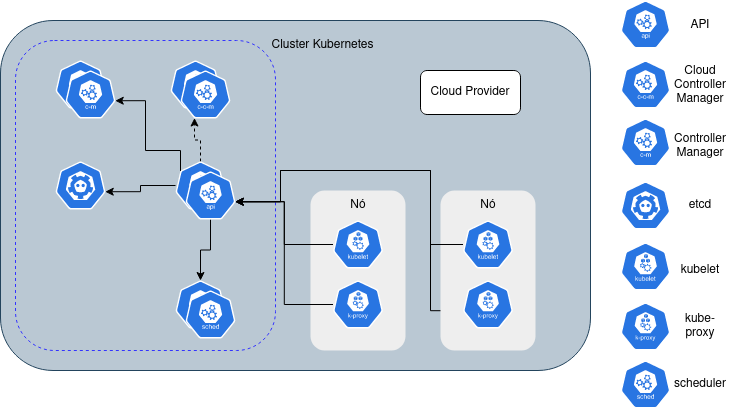
\includegraphics[scale=0.54]{images/kubernetes-components.png}
\label{fig:kubernetes:components}
\caption*{Fonte: Adaptado de \cite{kubernetes}.}
\end{figure}

Como visto na figura, temos diversos componentes que juntos trabalham para
prover as funcionalidades do \textit{framework} do Kubernetes:

\begin{itemize}
    \item kube-apiserver: é a API do Kubernetes, onde estão definidos os tipos
    de recursos que o \textit{cluster} possui, realiza a interface de acesso aos
    dados que ficam armazenados em banco de dados. Permite a criação e administração
    dos recursos através desta API através de acesso de dados CRUD (\textit{Create},
    \textit{Retrieve}, \textit{Update}, \textit{Delete}).
    \item etcd: não é desenvolvido pelo Kubernetes, mas, é utilizado para armazenar
    todos os metadados do \textit{cluster}, como por exemplo, em que nó um
    contêiner está sendo executado e quais outros contêineres podem acessar via
    HTTP este contêiner. Neste banco de dados de chave/valor também são armazenados
    o estado desejável dos recursos que o Kubernetes está administrando.
    \item kube-scheduler: aplicação que cuida da atribuição de um nó para um contêiner.
    Para escolher o melhor nó se faz uso de diversas políticas, como a definição dos
    recursos necessários do contêiner, é necessário que o nó possua os recursos e
    que os recursos gerais sejam utilizados da melhor forma no \textit{cluster},
    ou também se o nó possui alguma peculiaridade em anotação, como, por exemplo,
    uma GPU, o que é chamado de \textit{node affinity}.
    \item kube-controler-manager: todos os recursos da API do Kubernetes possuem
    um \textit{controller}(controlador) que controla a criação e administração
    destes recursos. Nesta aplicação, estão definidos a maioria dos controladores
    padrões do Kubernetes. Quando necessitamos estender a API, geralmente escrevemos
    novos controladores que executam separadamente destes.
    \item cloud-controller-manager: aplicação específica para \textit{clusters}
    que estejam sendo executados em serviços de nuvem, permitindo que o serviço defina
    como serão feitos os roteamentos de dados de rede e outras particularidades de
    acesso de rede na nuvem, por exemplo, abertura de portas e exposição das mesmas,
    protocolos de redes, DNS, entre outros.
\end{itemize}

Nem todo nó precisa executar o \textit{control plane}, mas, todos os nós que
executam contêineres do usuário precisam contar com três aplicações, o kubelet,
o kube-proxy e a \textit{runtime} de contêiner, como visto na Figura
\ref{fig:kubernetes:components}. O kubelet é responsável por administrar os
contêineres da máquina e assegurar que o contêiner é executado conforme a
definição de um Pod. Desta forma, é possível saber quais contêineres não são mais
necessários através das definições do estado almejado por cada recurso. O
kube-proxy implementa regras de rede para o nó que permitem que os contêineres
que este executa sejam acessíveis aos outros nós do \textit{cluster}, através
de registros DNS internos ao \textit{cluster}. Por fim, a \textit{runtime} de
contêineres é a responsável por de fato executar os contêineres do nó. O kubelet
se comunica com a \textit{runtime} de contêineres para que seja possível realizar
a administração dos contêineres, realizando ações que seriam feitas manualmente
por um usuário fora de um orquestrador, como escalar um contêiner.

\subsubsection{Pod}

O Pod é o conceito fundamental do Kubernetes. Um Pod é a encapsulação de
diversos contêineres de uma aplicação com significado lógico para estarem
executando juntos. Dentro de um Pod, as ferramentas do Linux, como cgroups e
namespaces, isolam os contêineres executando no Pod em um contexto
compartilhado, permitindo a comunicação entre os contêineres e compartilhamento
de recursos. O Pod é definido, como todo recurso do Kubernetes, através de um
arquivo YAML ou JSON, contendo a imagem que será utilizada, os recursos e
também os contêineres que serão utilizados \cite{kubernetes:pod}. O próprio
Kubernetes executa algumas de suas aplicações internas em Pods, como o próprio
kube-apiserver. Toda aplicação que executa no Kubernetes executa através de um
Pod, que é o recurso mínimo para que possamos utilizar o Kubernetes.

\subsubsection{Deployment/StatefulSet}

Para administrar Pods no Kubernetes utilizamos o Deployment ou o StatefulSet.
A principal diferença entre os dois é que o último permite a utilização de
volumes persistentes para armazenar dados entre reinicializações dos Pods.
Eles permitem definir os estado que queremos que nosso Pods permaneçam, este
estado está relacionado principalmente ao número de réplicas deste Pod e
também da versão de imagem de contêiner que eles devem estar. O Deployment
ou StatefulSet lida com toda a parte de criar novos Pods e seus contêineres,
de reiniciá-los, pará-los ou atualizá-los através de um controlador do
kube-controller-manager \cite{kubernetes:deployment}. Estes recursos permitem
que o Kubernetes possa administrar as aplicações que ele executa através de
outros recursos, como o ReplicaSet, que é a definição da quantidade de réplicas
que deve ser mantida para cada um dos serviços.

\subsubsection{Volumes}

Para o armazenamento de dados persistentes, o Kubernetes utiliza o conceito
de Volumes, que é uma abstração sobre uma localização de dados
persistentes. Existem diferentes tipos de volumes que permitem que sejam
utilizadas implementações de diferentes provedores de serviços em nuvem ou
até mesmo de discos rígidos das máquinas em que se está executando o
\textit{cluster} do Kubernetes \cite{kubernetes:volumes}.

Os Volumes do Kubernetes funcionam de maneira diferente dos do
Docker, sendo que no último é mais desorganizado, onde, é apenas disponível para o
disco local ou outro contêiner. Os Volumes do Kubernetes permitem
que seja compartilhando um volume entre diversos Pods através de permissões
dos volumes que são solicitadas para os Pods como PersistentVolumeClaim para os
PersistentVolumes \cite{kubernetes:persistent-volumes}. Nas reinicializações
de Pods com PersistentVolumeClaims é assegurado que eles receberão acesso
ao mesmo volume novamente, persistindo os dados armazenados da aplicação.
Isto não permite o salvamento de dados em memória, que não são salvos em
persistência de dados, mas, no contexto da aplicação.

\subsubsection{Controllers}

Todos os recursos definidos no Kubernetes são controlados pelos chamados
\textit{Controllers}. Estes controladores ouvem a mudanças nos estados dos recursos
a partir de monitoramento da API do Kubernetes, kube-apiserver, e executam passos
para atingir os objetivos de estado que os recursos na API necessitam. O
Kubernetes provê alguns recursos padrões, como Pods, Jobs e Volumes e
todos estes possuem um controlador para controlar o estado desejado de
cada um dos recursos \cite{kubernetes:controllers}.

Também podemos adicionar recursos através de controladores personalizados,
estes são criados em qualquer linguagem de programação e também se comunicam
com o kube-apiserver. Com isso, é possível estender, por exemplo, a
funcionalidade do StatefulSet Controller, a partir de monitoramento dos
recursos que ele administra. Com isso, podemos, por exemplo, adicionar novas
funcionalidades para monitorar Pods e criar funcionalidades como servidores
de \textit{reverse proxy} \cite{kubernetes:controllers}.

\section{Serviços Stateful e Stateless}

De modo geral, quando executamos uma aplicação ou um serviço em produção,
temos dois tipos de possibilidade de aplicações. Temos as aplicações que
não necessitam saber do estado de execução da aplicação, como, por exemplo,
a instrução que estava sendo executada. Aplicações que precisam
apenas acessar um banco de dados e servir dados, como uma API HTTP, não
possuem necessidade de permanecer o estado da memória ou mesmo de saber a
instrução sendo executada em determinado momento. Chamamos este tipo de
aplicação/serviço de \textit{Stateless}, ou seja, sem estado. A maioria das
aplicações desenvolvidas para microsserviços são desenvolvidas através
deste padrão \cite{vayghan2021kubernetes}.

No caso de aplicações mais críticas, que necessitam de um estado de execução,
como, por exemplo, uma aplicação que se comunica com clientes e mantém estado
do acesso de cada cliente e suas execuções em memória. Estas aplicações/serviços
nós chamamos do tipo \textit{Stateful}, ou seja, com estado. Estas, em geral,
tem menos tolerância a falhas, por exemplo, se ela falhar perdemos todo o estado
da aplicação e não teremos a mesma aplicação executando quando ela reiniciar,
é interessante que possamos de alguma forma salvar este estado nos casos de falha
\cite{vayghan2021kubernetes}.

O estado da aplicação em geral consiste do estado do processo pai e filhos
executando na aplicação. Este estado contém, por exemplo, como as páginas
de memória estão em determinado momento. Desta forma, temos exatamente o
estado da execução, mas, não temos conhecimento de como ela nele. Não seria
interessante para a aplicação salvar estes valores em persistência, pois,
seria necessária muita instrumentação \cite{oh2018stateful}.

\subsection{etcd}

O \textit{etcd} consiste de um banco de dados de chave/valor distribuído.
A distribuição e replicação dos dados se dá por um algoritmo de eleição de
líderes, logo, ele é tolerante a falhas e consistente. \cite{etcd}

Por se tratar de um banco de dados distribuídos, ele é adequado para
utilização em \textit{clusters}, e, por isso, é utilizado por padrão no
Kubernetes para armazenar metadados dos seus recursos. Também é comum que
controladores customizados do Kubernetes utilizem este para armazenamento
de seus metadados \cite{kubernetes:etcd}.

\section{Checkpointing/Restore}

A técnica de\textit{Checkpoint/Restore} permite o salvamento do estado de
uma aplicação \textit{Stateful} e, posteriormente, a restauração da
aplicação a partir do ponto de salvamento passado. Em geral a técnica
consiste em obter uma cópia da execução em memória da aplicação, salvar o
contexto em uma imagem que poderá ser armazenada em armazenamento sólido e
persistente. Quando há a necessidade de se recuperar o estado da aplicação
a imagem que temos é utilizada para recuperar o estado para o momento em
que ocorreu o salvamento da imagem \cite{laadan2010linux}.

Esta técnica pode ser utilizada para tolerância a falhas no caso de aplicações
que quando falham necessitam do estado de recuperação \cite{muller2022architecture}
\cite{Chen2015/10}, aplicações \textit{Stateful}. Nesta técnia temos cópias
dos estados anteriores da aplicação e podemos recuperá-la mais rapidamente.
Outra possibilidade também é aumentar a disponibilidade dos serviços através
do salvamento do estado e posterior recuperação dele \cite{vayghan2021kubernetes}.
Embora, a técnica de \textit{Checkpoint/Restore} tenha o objetivo de salvar um
estado e depois recuperá-lo, ela pode ser utilizada para outras finalidades não
envolvidas exatamente nessa linha, como migração de aplicações entre nós de um
\textit{cluster} \cite{Chen2015/10}.

\subsection{CRIU}

CRIU é um projeto que implementa \textit{Checkpoint/Restore} no Linux no
userspace, o acrônimo da aplicação se dá justamente por isso,
\textit{Checkpoint/Restore in Userspace}. Ele trabalha com o conceito de
congelar a execução de um processo, salvar seu estado de execução no disco,
que depois pode ser utilizado para recuperar a aplicação exatamente no
momento em que ela parou. Como contêineres são isoluções em cima das
ferramentas do Linux, é possível realizar o salvamento de estado de
contêineres utilizando o CRIU \cite{criu}.

Algumas \textit{runtimes} de contêineres possuem o suporte de
\textit{Checkpoint/Restore} implementado com o auxílio do CRIU, é o caso
do containerd. Por usar runc para construção do \textit{backend} da
\textit{runtime}, que possui o CRIU integrado, comandos na
interface de linha de comando do containerd foram criados para realizar o
\textit{Checkpoint/Restore}. Desta forma, utilizando o Kubernetes com
containerd também é possível realizar \textit{Checkpoint/Restore} dos
contêineres, não de forma nativa, mas se aproveitando das funcionalidades
do containerd através do CRIU e a comunicação com as APIs tanto do containerd
quanto do Kubernetes.

\section{Event Sourcing}

O padrão de projeto \textit{Event Sourcing} cria eventos sobre ações em um
sistema e, armazena estes em fluxos ordenados \cite{event-sourcing},
através de um versionamento da ordem. Então, quando uma ação é feita no sistema
temos a emissão de um novo evento para um determinado fluxo. Estes são ordenados
pela versão em que são entregues. Uma vantagem deste modelo é a possibilidade
de alcançar o estado da aplicação em um determinado momento apenas reprojetando
os eventos, ou seja, ao emitir os mesmos eventos em ordem até um determinado
momento no tempo, e, por momento se entende a última versão desejada
\cite{event-sourcing}.

Este padrão permite uma grande forma de auditoria ao armazenar as ações
feitas pelo sistema e permite encontrar incosistências com grande facilidade
ao reprojetar eventos até o ponto de uma falha. Também é possível adicionar
um \textit{snapshotter} que captura o estado do sistema em determinado
momento, e, não será necessário reprojetar todos os eventos desde de o início
do sistema, economizando tempo de processamento \cite{event-sourcing}.


    % Capítulo de Revisão Bibliográfica.
    
% The \phantomsection command is needed to create a link to a place in the document that is not a
% figure, equation, table, section, subsection, chapter, etc.
% https://tex.stackexchange.com/questions/44088/when-do-i-need-to-invoke-phantomsection
\phantomsection

% Multiple-language document - babel - selectlanguage vs begin/end{otherlanguage}
% https://tex.stackexchange.com/questions/36526/multiple-language-document-babel-selectlanguage-vs-begin-endotherlanguage
\begin{otherlanguage*}{brazil}
% ----------------------------------------------------------
\chapter{Trabalhos Relacionados}\label{cap:trabalhos:relacionados}
% ----------------------------------------------------------

Neste capítulo serão apresentados alguns trabalhos que possuem correlação
com esta monografia, envolvendo os conceitos de \textit{Checkpoint/Restore},
tolerância a falhas e contêineres.

\section{Checkpoint/Restore para contêineres Stateful}

Em \cite{muller2022architecture}, é proposto, como prova de conceito, uma
arquitetura transparente para realizar o \textit{Checkpoint/Restore} de
contêineres \textit{Stateful} utilizando Kubernetes. O foco primário é em
tolerância a falhas com técnicas de \textit{Checkpoint/Restore}, onde se é
abordado a problemática de se ter uma réplica nova do serviço que seja
consistente com o momento atual da falha, não havendo perda de informações
de estado da antiga réplica.

Para o \textit{Checkpoint/Restore} o trabalho propõe a utilização de um
contêiner \textit{sidecar}, o interceptador, que intercepte as requisições
para o contêiner que será feito o \textit{Checkpoint/Restore}. Este contêiner
irá redirecionar as requisições ao contêiner que é feito o \textit{checkpoint}
e também controla o momento do \textit{checkpoint}. Desta forma, é possível
saber quais as requisições que foram processadas pelo contêiner que está sendo
monitorado até o momento do último \textit{checkpoint}, já que a imagem de
\textit{checkpoint} possui metadados salvos no \textit{etcd}. Quando uma nova
réplica deste contêiner for iniciada, teremos a imagem do último
\textit{checkpoint} e o interceptador irá refazer as requisições feitas a
partir do momento do último \textit{checkpoint}, isto permite obter a imagem
mais consistente com o momento da falha do último contêiner que estamos
reinicializando.

Na arquitetura também temos um operador, que é responsável por manter o
estado das aplicações, ele troca informações com o interceptador para remover
contêineres, reiniciá-los ou avisar que eles falharam. Outro ponto da
arquitetura é o administrador de estados, que serve para armazenar e categorizar
as imagens do \textit{checkpoint} com \textit{checksums} e seus metadados no etcd.

Na proposta, se utiliza um monitoramento por \textit{ping} de pacotes para
identificar se um contêiner falhou ou não. No próprio trabalho o autor deixa
claro outros métodos que poderiam ser utilizados, como monitoramento das
informações do contêiner, ou mesmo um indicador de saúde provido pelo contêiner.
A partir do momento de identificação da falha, outro contêiner com a imagem
mais recente de \textit{checkpoint} é criado para substituir o contêiner
falhante. Como o interceptador só confirma uma mensagem quando o contêiner
responde de volta, então, temos certeza de que o interceptador sabe a partir
de qual requisição enviar para recuperar o estado.

Por fim, é apresentada uma prova de conceito realizada em cima do Kubernetes.
A partir da prova de conceito o controlador do StatefulSet foi estendido para
dar suporte ao Operador da arquitetura, e a aplicação a ser monitorada e o
Interceptador foram colocados no mesmo Pod. Conseguiu-se provar ao utilizar o
Kubernetes a possibilidade de utilizar a arquitetura para
\textit{Checkpoint/Restore} para tolerância a falhas. Mas, foram levantados
pontos de melhoria, como, utilização de \textit{checkpointing} ativa, ou seja,
realizando \textit{checkpoint} somente quando uma réplica falhar, para diminuir
o problema de \textit{buffer} em cache dos interceptadores, detecção de falhas
a partir de processos diferentes, como um algoritmo Bizantino, e outros
processos de recuperação pró ativa, como votação para decidir réplicas incorretas.

No contexto do trabalho desenvolvido por nós, este trabalho propõe pontos
importantes para nosso desenvolvimento. Como, por exemplo, como recuperar
exatamente o estado que precisaríamos do nosso serviço. Também é interessante
a abordagem para salvamento de metadados utilizando o etcd que já vem integrado
ao Kubernetes. Nota-se, também, que alguns pontos de melhoria podem ser
priorizados no desenvolvimento de nosso trabalho para ter uma solução mais
abrangente de outras aplicações.

Já em \cite{vayghan2021kubernetes}, os autores propõe uma extensão das
funcionalidades do Kubernetes para contêineres \textit{Stateful} para
prover alta disponibilidade (\textit{High Availability}) à réplicas de um mesmo
microsserviço. Isto implica, que será necessário manter a aplicação disponível
o mais rápido possível depois de ela ter alguma falha.

O trabalho em \cite{vayghan2021kubernetes} aborda uma nova forma de se
utilizar contêineres \textit{Stateful} sem utilizar o StatefulSet do Kubernetes,
mas utilizando o Deployment com um Persistent Volume compartilhado entre todos
os Pods dos quais o Deployment controla. Desta forma, todos os contêineres
compartilham o mesmo armazenamento e tem acesso ao mesmo estado em disco.
Segundo o artigo, nenhum dos dois tipos conseguem suprir necessidades reais de
aplicações de alta disponibilidade, por isso, se faz necessário criar uma
solução que provenha mais velocidade na reinicialização de Pods falhantes.

A solução proposta consiste em ter dois Pods disponíveis provendo o mesmo
serviço em determinado tempo. Um deles é classificado como o ativo, enquanto
o outro é classificado como o "em espera". O Pod que serve requisições é o
ativo, quando este falha um \textit{controller} criado para isso, State Controller,
copia o estado do Pod falhante para o Pod reserva e cria um novo Service para ele
servir as requisições. Quando o Pod ativo é recuperado, se faz o caminho inverso
para ele voltar a ser o Pod que recebe as requisições. A replicação de estado no
Pod reserva é feito através de um redirecionamento das requisições do Pod ativo,
como o State Controller cria Services separados para os Pods é possível descobrir
o Pod reserva através do nome do Service ao invés de seu IP no \textit{cluster}
graças ao componente de kube-proxy do Kubernetes.

Por fim, são apresentados os experimentos e resultados, tendo em mente que a
alta disponibilidade dos serviços almejada era de 99,999\% anualmente. Os
experimentos consistiram em utilizar um serviço de \textit{streaming} para os
clientes, em que o estado do contêiner consiste no momento que o cliente está
na transmissão de vídeo, utilizando um cluster de oito máquinas e salvando o
estado num Persistent Volume.

As métricas de disponibilidade usadas foram de tempo de reação, o tempo de
reação do Kubernetes para perceber uma falha e iniciar o processo de
recuperação do Pod, o tempo de reparo, tempo a partir da percepção do Kubernetes
até recuperação do Pod, o tempo de recuperação, o tempo a partir da percepção
da falha pelo Kubernetes até a finalização da recuperação e quando o serviço
atinge o estado de pronto, e, por fim, o tempo de indisponibilidade, que
consiste no tempo que o serviço permanece sem disponibilidade, representado
pela soma do tempo de reação com o tempo de recuperação.

Outras métricas obtidas pelo serviço, o State Controller proposto também
foram utilizadas. A métrica de tempo de escala, que é o tempo de percepção
do controlador de estado de um evento de escala até o escalonamento e
disponibilização do serviços escalados para mais ou menos réplicas. A métrica
de tempo de configuração do estado de alta disponibilidade, que é o tempo
para o State Controller agir de acordo com o evento de réplica e configurar
os estados dos Pods para se ter um ativo e outro reserva.

Os experimentos pretendiam responder às cinco perguntas:

\begin{enumerate}
    \item Qual o impacto do State Controller na disponibilidade provida?
    \item Qual o impacto de escalar durante um momento de falha na
    disponibilidade que o State Controller pode prover aos microsserviços
    gerenciados?
    \item Qual é a sobrecarga gerada pelo State Controller no escalonamento?
    \item Qual é o impacto de falhas simultâneas nos Pods ativos no tempo de
    indisponibilidade de cada Pod falhante?
\end{enumerate}

Dos experimentos se obteve respostas:

\begin{enumerate}
    \item Os resultados mostram que é mais rápido para o State Controller
    configurar os estados aos Pods recuperados do que o Kubernetes recuperar
    os serviços. Com uma pequena diferença na velocidade de recuperação entre
    StatefulSets e Deployments, onde o último tem velocidade maior e melhorada
    graças ao State Controller. Apesar do pequeno trabalho a mais que o State
    Controller gera o tempo de recuperação diminui devido ao Pod reserva.
    \item Os resultados mostram que o State Controller gera um atraso no
    escalonamento devido ao tempo que se leva para configurar os estados de
    disponibilidade aos Pods. Como o serviço não consegue realizar as duas
    operações ao mesmo tempo, ocorre um atraso no escalonamento, com maior atraso
    para os escalonamento de menos réplicas.
    \item Os resultados mostram que gera mais trabalho para escalonamento, mesmo
    sem falhas, e que demora mais para as reações de escalonamento ocorrerem
    quando se utiliza o State Controller.
    \item Os resultados mostram que quanto mais tarde um Pod falha mais tarde ele
    será recuperado pelo State Controller, isto ocorre, segundo a autora, pela
    utilização de uma fila \textit{FIFO} para tratamento da recuperação, o que
    gera este problema.
\end{enumerate}

Este trabalho demonstra uma outra forma de abordar o problema de serviços
\textit{Stateful}, ao invés de se salvar o estado em memória, se salva o
estado utilizando os métodos de Persistent Volumes do Kubernetes. Desta
forma, demonstra mais um fator que pode ser interessante observar no
desenvolvimento do nosso trabalho, já que, para algumas aplicações este
estado é interessante. Outro fator importante é a seleção de métricas, que
o artigo aponta algumas métricas importantes para se considerar na avaliação
da adequação da solução.

Já em \cite{schmidttransparent}, temos uma proposta de uma ferramenta para
tolerância a falhas em contêineres \textit{Stateful} no Kubernetes utilizando
\textit{Checkpoint/Restore}. Os autores utilizam a técnica de \textit{Checkpoint}
já disponível no Kubernetes em versão alpha para gerar um ponto de salvamento
do estado do sistema. O Kubernetes utiliza a \textit{runtime} de contêineres
cri-o\cite{cri-o}, que internamente, utiliza o CRIU\cite{criu} para realizar
o \textit{Checkpoint}. Como os autores discutem, este ponto de salvamento
gerado não pode ser utilizado diretamente para executar outro contêiner como
uma imagem.

Para possibilitar a parte do \textit{Restore} os autores desenvolveram uma
aplicação que constrói uma imagem compatível com \textit{Open Container Interface}
que é possível ser utilizada no cri-o. Para o desenvolvimento tanto do sistema
de \textit{Checkpoint} quanto do de \textit{Restore} os autores utilizaram o
conceito de operador do Kubernetes para monitorar o estado dos recursos do 
\textit{cluste} e conciliar para salvar o estado das aplicações monitoradas
através de anotações nos manifestos dos recursos e restaurar quando ao monitorar
se perceber que houve uma falha na aplicação monitorada. Foram integradas outras
funcionalidades ao trabalho, como a possibilidade de integrar diversos nós do
\textit{cluster} para distribuição geográfica e possibilidade de criar formas
diferentes de se verificar se a aplicação falhou, como um recurso de
\textit{liveness}.

Os autores conseguiram prover o serviço, que, como já esperado gera um pouco
de perda de performance nos momentos de realizar o salvamento do estado e da
recuperação. Também é possível ver que durante momentos de salvamento e de
recuperação a latência das aplicações aumenta, pois, durante um
\textit{Checkpoint} a aplicação fica não responsiva, e até a recuperação da
aplicação falhante há outra latência. Entretanto, se verificou que é possível
realizar o \textit{Checkpoint/Restore} de aplicações \textit{Stateful} no
Kubernetes.

\section{Checkpoint/Restore com migração de contêineres Stateful}

Em \cite{oh2018stateful}, os autores desenvolvem uma técnica de
\textit{Checkpoint/Restore} para migração de \textit{clusters} com contêineres
StatefulSet. Como prova de conceito é construída uma aplicação em cima de
Kubernetes e CRIU para realização do \textit{Checkpoint/Restore}. Alguns
motivos levam um contêineres em um orquestrador de contêineres ter que ser
movido de um nó para outro, como manutenção do nó atual necessitando de uma
reinicialização, falha do nó atual ou escalonamento e balanceamento de carga
das aplicações do \textit{cluster}. Logo, se um contêiner possui estado,
nestes casos é interessante que a migração dele para um novo nó seja feita
com salvamento do estado passado para reinicializar consistentemente.

Primeiramente, é analisada uma técnica para migração de contêineres
\textit{Stateful} através da utilização de volumes, \textit{Persistent Volumes}
no Kubernetes. Através da análise do autor, se observa que para realizar
uma migração do estado utilizando os volumes, se tem uma complexidade aumentada.
Já que, para salvar o estado em um volume é necessário que a aplicação saiba
realizar esta tarefa, então, não é transparente ao desenvolvedor. Também o
desgaste pelo acesso ao volume que pode ser intermediado por uma API de terceiro,
como no caso de um volume de dados armazenado na EC2 API da Amazon. A partir
desta análise, os autores propõe uma abordagem através da técnica de
\textit{Checkpoint/Restore} com criação de uma imagem com o estado salvo do contêiner.

Para realização da migração eles propõe uma solução que consiste em três
estágios: pré migração, migração e pós-migração. Na pré migração é iniciado
o processo de migração por qualquer motivo, como escalonamento, depois se elege
novos nós para receberem os contêineres do nó antigo, por fim, se criam as
imagens dos contêineres para substituir as antigas. Na migração é realizado
\textit{checkpoint} do contêiner, gerando uma nova imagem, esta imagem é
transmitida para o novo nó através da internet e no novo nó é iniciado um
novo contêiner a partir desta imagem, isto permite que o processo seja
resumido com seu estado passado. Por fim, no estágio de pós migração é
realizada a alocação de recursos antigos, como balanceadores de carga ou
registros \textit{DNS} para o novo contêiner.

Segundo os autores, a solução proposta ainda possui alguns problemas. No
caso de falhas do nó ela não consegue realizar a migração, embora
\textit{checkpoint} periódico resolveria esta dor, problemas com a internet
para envio da imagem são ignorados. Mas, com a proposta se pode obter uma
transparência a nível de aplicação da migração do contêiner, se tem uma
migração leve e ágil, já que, não se usa um volume e, não tem o trabalho
a mais de comunicação com possíveis APIs externas e leitura/escrita de volumes.

Para testar a solução se utilizou um \textit{cluster} de máquinas com um
orquestrador de contêineres e uma aplicação de servidor que incrementava
um contador a cada requisição com o estado salvo em memória. Também se
implementou a solução na linguagem Go, se comunicando com a \textit{engine}
Docker e utilizando o CRIU para realizar o \textit{checkpoint}. Como
observado no trabalho, o tempo de inatividade no processo de migração se
mostra baixo, 576.61 em média, sendo que o tempo de latência da aplicação
não foi alterado durante a utilização da imagem. Também não houveram
falhas para enviar a imagem de \textit{checkpoint} pela rede para o novo nó.

Embora neste trabalho o conceito abordado de \textit{Checkpoint/Restore}
seja utilizado em um contexto diferente, para migração de aplicações em
\textit{clusters}. Ainda sim, muitos conceitos se relacionam a nosso trabalho.
A utilização de contêineres e aplicações de \textit{Checkpoint/Restore},
diferentemente dos outros trabalhos vistos até o momento, este utiliza uma
outra forma de salvar a imagem de \textit{checkpoint}, que é através do envio
pela rede. Também é abordada a transparência da aplicação, que também é
importante no nosso trabalho, para que não haja adaptação das aplicações
para a solução específica. Por fim, os autores apontam para um ponto
importante que queremos cobrir, que é o caso de tolerância a falhas no caso
de uma falha de nó, como apontado por eles, que por sugestão dos autores
poderia ser resolvida por monitoramento do nó ou mesmo \textit{checkpoints}
periódicos das aplicações com estado.

Já em \cite{tran2022proactive}, os autores propõe uma implementação
para migração de serviços \textit{Stateful} que seja proativa, ou seja,
que perceba antes de uma falha ocorrer no nó e realize a migração para
um novo nó sem que haja a necessidade do nó falhar antes, isto aumenta
a tolerância a falhas e a qualidade de serviço provida. Para isso, os
autores utilizam um algoritmo de \textit{Bidirectional Long Short-Term
Memory} (Bi-LSTM) para predição de falhas. A seleção foi em base do estado
da arte em \textit{Machine Learning}, já que o propósito do artigo é
avaliar a atividade proativa de \textit{Checkpoint/Restore} para
migração dos contêineres. Desta forma, se utilizou o algoritmo para prever
a sobrecarga do uso de CPU como falha.

Para realizar o \textit{Checkpoint/Restore} os autores propõe uma solução
baseada no StatefulSet do Kubernetes, assim como em \cite{vayghan2021kubernetes},
e também um salvamento dos dados em memória através do CRIU, como em
\cite{muller2022architecture}. Desta forma, se tem o estado total da aplicação,
suportando multi \textit{clusters} e \textit{clusters} de nó único.

Para realização das migrações proativas foram criados três aplicações
principais. O \textit{Monitor Framework}, responsável por monitorar as métricas
do \textit{cluster}, como CPU e memória, também lida com o registro de serviços.
O \textit{Fault Prediction Framework}, responsável pelo modelo de predição
de falha, que possui dois processos, o processo \textit{offline}, que realiza
o treinamento com base nos dados recebidos do \textit{Monitor Framework} sobre
a métrica de CPU, e, o processo \textit{online}, que realiza a execução do
modelo com a predição da falha do nó. Por último, temos a funcionalidade
nativa de migração de \textit{clusters}, que é uma modificação do Kubernetes,
componente kubelet, para possibilitar a utilização da predição e da migração
entre dois \textit{clusters}. Podemos ver esta arquitetura demonstrada na
Figura \ref{fig:proactive}.

\begin{figure}[h]
\centering
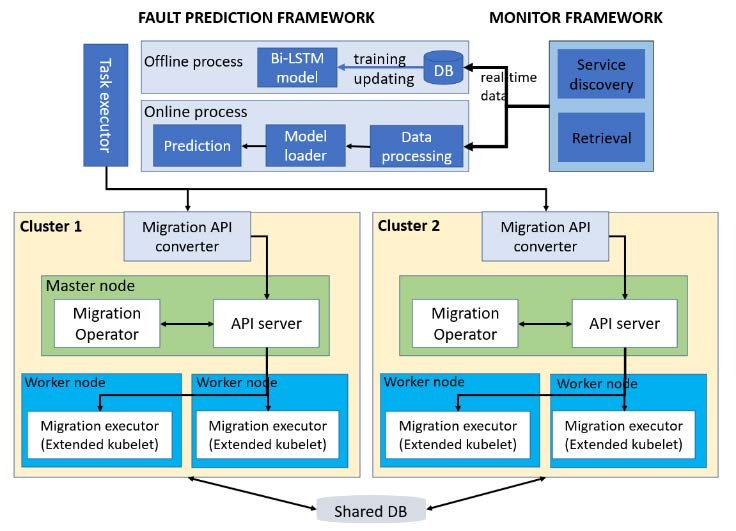
\includegraphics[scale=0.54]{images/proactive-architecture.png}
\caption{Arquitetura de migração proativa de contêineres em \textit{clusters}.}
\label{fig:proactive}
\fonte{\cite{tran2022proactive}}
\end{figure}

Para realizar a migração foi modificado o componente kubelet do Kubernetes e
também a \textit{runtime} de contêineres em utilização pelo Kubernetes para
possibilitar a comunicação com o CRIU para realizar o \textit{Checkpoint/Restore}
dos processos dos contêineres a serem migrados. Desta forma, quando uma migração
é solicitada, primeiro se realiza o \textit{Checkpoint/Restore} de todos os
contêineres no Pod solicitado para migrar, depois se envia a imagem ao novo nó
que ele irá executar. O novo nó utiliza a imagem gerada do \textit{Checkpoint}
para restaurar o estado antigo, só então são excluídos o Pod antigo e
redirecionado o Service ao novo.

Para o processo de migração se utilizou o conceito de Operator do Kubernetes
e \textit{Custom Resource Definitions} (CRDs), que permitem a definição de
novos recursos de API e da criação de novos controladores para monitorar a
API e alcançar o estado desejado dos recursos. Então, em um processo de
migração um novo recurso de migração é adicionado ao Kubernetes e o
controlador da migração deve ser capaz de realizar o Checkpoint do Pod, enviar
para o novo nó, iniciar o Pod no novo nó, eliminar o Pod antigo e reconfigurar
o Service para o novo Pod. Também alteraram a definição da interface de
\textit{runtime} de contêiner do Kubernetes para incluir métodos para realizar
\textit{Checkpoint} e \textit{Restore} com CRIU, desta forma, é possível realizar
as chamadas diretamente pela API do Kubernetes. Por fim, foi utilizado um servidor
de arquivos para armazenar as imagens de \textit{Checkpoint} entre os nós de
migração, desta forma, basta montar o volume nos dois nós e eles estariam
compartilhando as imagens, desta forma, também se remove a necessidade de envio
por internet da imagem entre os nós e diminui as comunicações.

Para realizar a validação da solução se utilizou quatro \textit{clusters} de
Kubernetes, onde seriam executados aplicações de longo período de inicialização,
como \textit{Mongo-DB} e \textit{Redis}, bem como aplicações de estado baseado na
execução, como FFMPEG, todas executando através de StatefulSets. Para realizar a
migração proativa, o estresse de CPU foi simulado utilizando uma ferramenta que
permite sobrecarregar os nós, \textit{Stress-ng}. Assim, foram verificadas métricas
para resultados, no caso o erro da média da raiz quadrado e o erro de média absoluta
para o modelo de predição e o tempo de recuperação do serviço migrado e a latência
de qualidade de serviço evitada pela migração.

Como resultados foi observado que dos modelos abordados o melhor para a predição
correta através de dois processos é o Bi-LSTM e ele pode ser utilizado para séries
de tempo de diferentes tipos, como CPU, memória e temperatura. Também se observou
que nas aplicações com tempo longo de inicialização houve melhoria do tempo de
recuperação de serviço apenas em redes de alta velocidade, mas, segundo os autores
não é um problema devido as novas redes de alta disponibilidade e velocidade 5G e
6G. Outros dois fatores a se destacar para serviços de tempo de inicialização alto
é o que em momentos que o algoritmo de predição demora para prever a falha do nó
a migração pode não terminar e temos uma violação da qualidade de serviço em latência,
assim, como no caso de \textit{clusters} muito grandes, com muitos Pods, ocorre
degradação da comunicação com os servidores de arquivos das imagens, já que a rede
do \textit{cluster} fica sobrecarregada, o interessante para isto não ocorrer é
aumentar os servidores de arquivo e utilizar balanceadores de carga. Agora, para
as aplicações de estado em execução se observou que o tempo de recuperação foi
considerado com base em quanto o serviço demorava para completar suas funções, no
caso do padrão do Kubernetes tínhamos mais tempo gasto em recuperar por exemplo
todos os passos de uma conversão de vídeo no FFMPEG, já na migração a conversão
reiniciava do ponto do \textit{Checkpoint}, isto gerou uma melhoria de 20\% a 22\%
na qualidade de serviço em latência. Desta forma, se demonstrou que a migração
proativa com \textit{Checkpoint/Restore} pode melhorar a qualidade de serviço e
também tempos de recuperação dos serviços.

As mudanças nas características do Kubernetes abordadas no trabalho através de
Operators são de grande importância para este e indica um caminho a se seguir.
Também é interessante verificar as medidas feitas para avaliar a eficiência da
solução em questão de tempo de recuperação e variação da latência do serviço. Já
o modelo de predição não deve ser abordado em nosso trabalho, já que o foco não
é realizar a predição, isto poderia ser adicionado em um trabalho futuro.

\end{otherlanguage*}


    % PARTE
    % \ifforcedinclude\else\part{\lang{Implementation}{Implementação}}\fi
    % \label{segunda_parte}
    
    % Capítulo da apresentação do Serviço.
    
% The \phantomsection command is needed to create a link to a place in the document that is not a
% figure, equation, table, section, subsection, chapter, etc.
% https://tex.stackexchange.com/questions/44088/when-do-i-need-to-invoke-phantomsection
\phantomsection

% Multiple-language document - babel - selectlanguage vs begin/end{otherlanguage}
% https://tex.stackexchange.com/questions/36526/multiple-language-document-babel-selectlanguage-vs-begin-endotherlanguage
\begin{otherlanguage*}{brazil}

\chapter{\lang{Service}{Serviço}}\label{cap:servico}

Neste capítulo, abordamos a conceituação do nosso serviço de
\textit{Checkpoint/Restore} de contêineres \textit{Stateful} no Kubernetes.
Apresentamos a arquitetura geral do serviço e como os componentes da arquitetura
se comunicam entre si. Também é apresentado as duas implementações que foram
abordadas no trabalho, uma utilizando técnicas de \textit{Event Sourcing} e a
outra utilizando técnicas mais difundidas para \textit{Checkpoint/Restore} através
da utilização de CRIU para salvamento do estado de uma aplicação. Serão apresentados
ao longo do texto diagramas de sequência que representam o funcionamento da
arquitetura.

\section{Arquitetura Geral}

A arquitetura do serviço possibilita o \textit{Checkpoint/Restore} transparente das
aplicações monitoradas pelo serviço no Kubernetes. Esta arquitetura é agnóstica sobre
a implantação, seja ela em Kubernetes ou localmente em um sistema, é fortemente inspirada
pelo trabalho em \cite{muller2022architecture}. A arquitetura é possível de implementar
de diferentes formas, como na utilização de CRIU quanto de técnicas de
\textit{Event Sourcing}. Esta arquitetura também é adequada para execução em
\textit{cluster} de máquinas e adequada para microsserviços \citep{vayghan2021kubernetes}
\cite{muller2022architecture} \cite{oh2018stateful}, embora ainda falte um pouco de
compreensão de como poderemos utilizar ela em sistemas distribuídos geograficamente
de forma eficiente.

\subsection{Checkpoint/Restore}

O \textit{Checkpoint/Restore} de aplicações \textit{stateful} em contêineres podem ser
feitas entre duas formas, como abordamos no \ref{cap:fundamentacao:teorica}, ou
utilizando técnicas de salvamento do contexto dos processos, com isolação do contexto
provida para contêineres \cite{muller2022architecture} com CRIU, ou com as técnicas de
\textit{Event Sourcing}. No nosso serviço a parte de recuperação dos estados será
administrada pelo componente de Administrador de Estado, já a parte de salvamento de estado
será feita ativamente pelo Interceptador. Juntos estes dois componentes fornecem a
funcionalidade de salvamento do estado da aplicação e posterior recuperação em caso
de falhas.

\subsection{Armazenamento}

Para realizar os salvamentos de estados pelo Interceptador, é interessante que eles sejam
feitos de forma periódica, capturando o estado da aplicação em determinado ponto da execução.
Desta forma, é necessário armazenar este estado em algum armazenamento, podemos utilizar. Para
isso teremos a imagem gerada por \textit{Checkpoint} que deverá ser armazenada em algum lugar
para ser posteriormente recuperada, em \cite{vayghan2021kubernetes} utiliza-se o conceito de
volumes para armazenamento dos dados, aqui também iremos utilizar o mesmo conceito, tanto para
imagens de \textit{Checkpoint} quanto para armazenamento de eventos.

Ainda na questão do armazenamento, para utilização de \textit{Checkpoint} com CRIU,
diferentemente do \textit{Event Sourcing} é interessante sabermos metadados sobre o momento
de salvamento da imagem, que nos ajudem a identificá-la no tempo \cite{oh2018stateful}
\cite{muller2022architecture} \cite{Chen2015/10}. Para isso, nos trabalhos de
\cite{muller2022architecture}, \cite{oh2018stateful} e \cite{Chen2015/10} utilizou-se
bancos de dados distribuídos de chave/valor como o etcd. Nosso administrador de estado também
utilizará o mesmo conceito para armazenar metadados das imagens.

\subsection{Recuperação ao último estado}

Durante um salvamento do estado da aplicação a aplicação permanece indisponível para
servir requisições e comandos do usuário, pois, as técnicas de salvamento de estado
de contêineres com CRIU congelam o processo da aplicação para salvar o estado
\cite{vayghan2021kubernetes}. Já no \textit{Event Sourcing} não possuimos este problema.
Entretanto, no segundo caso precisamos saber a ordem em que as requisições chegam para
podermos reprojetar o estado da aplicação a partir da reemissão das requisições à aplicação
monitorada. Ainda no caso do CRIU, ainda precisamos saber quais as requisições que chegaram
a partir de um salvamento de estado, já que todas requisições posteriores àquele salvamento
não estaram no estado salvo, precisaremos replicá-las para o serviço monitorado também. De
modo geral, o que temos de diferença é que no caso do CRIU reprojetamos apenas as requisições
a partir do último ponto de salvamento, já no caso do \textit{Event Sourcing} replicamos
as requisições desde o começo da existência da aplicação.

Para solucionar o problema de alcançar o último estado possível da aplicação em uma
recuperação para nossos dois casos, iremos utilizar no nosso Interceptador o padrão de projeto
de Embaixador(\textit{Ambassador}) como em \cite{muller2022architecture}. Nosso Interceptador
irá interceptar as requisições que chegam a nossa aplicação monitorada, irá salvar cada uma
das requisições em um volume, que pode ser em memória ou armazenamento persistente, e
encaminhá-las a aplicação. Sempre que formos realizar uma restauração iremos replicar as
requisições a partir do último ponto de salvamento para utilização de CRIU, como em 
\cite{muller2022architecture}, mas, no caso do \textit{Event Sourcing} faremos uma
reprojeção total com todas as requisições feitas desde o momento que a aplicação começou a
executar.

Para que novas requisições que chegarem durante o processo de restauração não interfiram na
ordem do estado com as requisições sendo refeitas. Nosso Interceptador tem dois estados de
operação um Ativo que está enviando requisições diretamente para a aplicação monitorada, e
outro de Aguardo que ficará esperando a restauração terminar para começar a enviar as
requisições, neste estado as requisições não serão respondidas imediatamente aos clientes,
mas, só após a restauração finalizar, quando o estado do Interceptador retornar para Ativo.
Em \cite{vayghan2021kubernetes} algo semelhante foi feito sobre estados da aplicação sendo
recuperada para impedir que requisições cheguem com estado desatualizado da aplicação.


\subsection{A Arquitetura}

As subseções acima trouxeram um pocuo dos problemas que temos que enfrentar e como
resolvemos cada um dos problemas com algum componente do sistema. Nesta subseção, iremos
abordar um pouco de como os componentes se comunicam entre a arquitetura e delimitar as
funcionalidades de cada um dos componentes sem abordar nenhum tipo de implementação
específica. Aqui, abordamos o que o Administrador de Estado, o Interceptador, o Volume, o
Banco de dados e Conêiner são e fazem. A arquitetura de maneira geral está apresentada na Figura
\ref{fig:abstract-architecture}, e a chamamos de representação geral abstrata da arquitetura.

\begin{figure}[h]
\centering
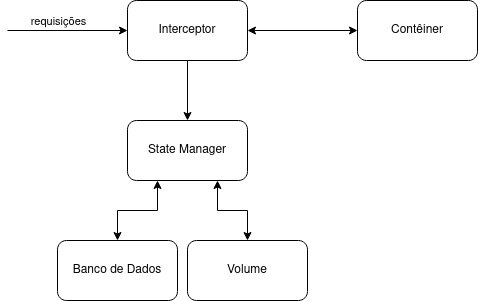
\includegraphics[scale=0.54]{images/abstract-architecture.png}
\caption{Representação da arquitetura abstrata da solução representada através de seus componentes.}
\label{fig:abstract-architecture}
\end{figure}

O Contêiner é a abstração da nossa aplicação com estado, que é o cerne deste trabalho
prover tolerância a falha a contêineres através de \textit{Checkpoint/Restore}. Este Contêiner
contem uma imagem executando, onde o endereçamento de memória é importante para o contexto
de execução da aplicação \cite{Chen2015/10}. A aplicação neste caso pode ser um banco
de dados como Redis ou uma aplicação de \textit{streaming} de vídeo como usado em \cite{vayghan2021kubernetes}.

O Volume é a abstração de um armazenamento persistente ou não para armazenar as imagens e
dados da aplicação. Para o nosso serviço é interessante que este Volume seja acessível
por diversas máquinas em diferentes localidades \cite{vayghan2021kubernetes}, pelo foco
do trabalho em \textit{clusters} de máquinas. Este volume deve permitir escritas das imagens
e recuperação das imagens através de uma interface de acesso.

O Banco de Dados é abstração de um banco de dados específico, este banco de dados precisa
persistir os dados, possibilitar a escrita, leitura e atualização dos dados. Ele também
deve ser distribuído pelo \textit{cluster} e tolerante a falhas para que todos as instâncias
dele consigam servir as mesmas informações consistentemente.

O Interceptor é a nossa aplicação do padrão de projeto do Embaixador \cite{ambassador}. Ele
deve interceptar as requisições a nossa aplicação, enviá-las ao Contêiner, esperar a resposta
deste, salvar a requisição para posterior recuperação das requisições respondidas pelo
Contêiner e responder para o cliente da requisição. Outro requisito do Interceptor é que ele
consiga replicar as requisições a um Contêiner a partir de uma informação de tempo, para que
possamos recuperar um estado do Contêiner apenas repetindo as requisições. O Interceptor também
é o responsável por realizar o salvamento do estado em uma imagem do Contêiner e enviar ao
Administrador de Estado os metadados da última requisição tratada, enquanto se faz um salvamento
também devemos colocar as requisições que chegarem em um \textit{buffer}, a partir da informação
do estado do Interceptador como Aguardo.

Por fim, o Administrador de Estado é o coordenador de toda a operação de
\textit{Checkpoint/Restore}, ele é quem deve receber metadados sobre a aplicação que tem salvamento
de estado feito. Também é o Administrador de Estados que realiza a principal funcionalidade sobre
o processo de restauração que é a identificação da falha do Contêiner monitorado e a atividade de
recuperação pela comunicação com o Interceptador.

\section{Arquitetura com Kubernetes} \label{subsection:kubernetes-architecture}

Para estruturação da arquitetura proposta na Subseção passada no Kubernetes devemos
fazer algumas modificações. Iremos primeiro revisar alguns conceitos abordados no
Capítulo \ref{cap:fundamentacao:teorica}. No Kubernetes temos o conceito de Operator,
eles permitem estender as funcionalidades do Kubernetes, aliados com a API do
Kubernetes podemos monitorar eventos no estado dos recursos e agir de acordo com isso.
Já sabemos que toda aplicação no Kubernetes executa através de um Pod, e, a forma de
realizar a criação e administração de um Pod é através de Deployments e ReplicaSets,
podemos monitorar estes recursos para criar novos Pods e verificar a falha deles.
Também temos PersistentVolumes no Kubernetes que são acessíveis através de todo o
\textit{cluster} e o etcd como banco de dados de chave/valor distribuído disponível
no Kubernetes. Representamos a arquitetura em Kubernetes na Figura
\ref{fig:kubernetes-architecture}.

\begin{figure}[h]
\centering
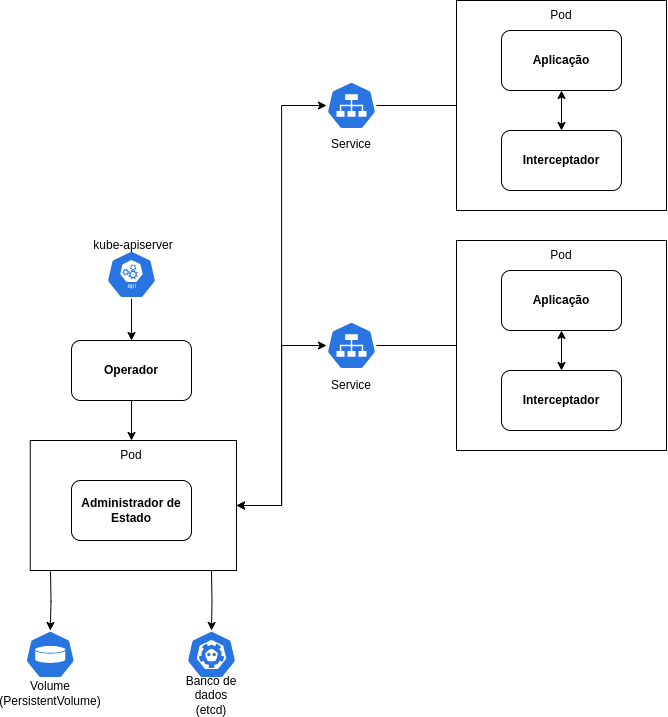
\includegraphics[scale=0.46]{images/kubernetes-architecture.png}
\caption{Representação da arquitetura da solução no Kubernetes.}
\label{fig:kubernetes-architecture}
\end{figure}

O Contêiner da aplicação será implantado a partir de um Deployment do Kubernetes, isto
permite definir a aplicação para ser administrada pelo Deployment usando ReplicaSets.
Com isto, teremos a distribuição do serviço e conseguiremos monitorar a criação, deleção
e atualização dos Pods que o Deployment e o ReplicaSet monitoram através da API do
Kubernetes. Como em \cite{schmidt2023state}, deveremos monitorar e modificar as
funcionalidades do ReplicaSet para possibilitar que nós possamos iniciar novos Pods
da aplicação com imagens recuperadas e identificar quais Pods devemos monitorar com
o nosso Interceptador.

Para implementação do Admnistrador de Estado iremos utilizar também o conceito de Operator
no Kubernetes. O nosso Administrador de Estado será implantado através de um controlador do
estado dos Pods, estes Pods sempre que tiverem uma alteração no seu estado como a falha, iremos
realizar a recuperação do estado. O administrador irá se comunicar com o Interceptador através
do endereço IP do Pod do Kubernetes que pode ser obitdo a partir do momento em que o Pod está
executando e pronto.

Nosso Interceptador será implantado através de um \textit{sidecar container} na aplicação
monitorada, teremos um Operador do Kubernetes que tentará conciliar o estado dos Deployments,
sempre que houver um Deployment com uma anotação do tipo \texttt{crsc.io/checkpoint-restore}
com valor de \textit{true}, iremos criar um novo contêiner no deployment que servirá como 
Interceptador e irá interceptar o tráfego ao Pod. Assim, como em \cite{muller2022architecture},
nosso Interceptador implementado como um \textit{sidecar} permite economia de tráfego, já que
ambos os contêineres operando no Pod tem a mesma interface de rede.

Para o Interceptor é importante que alguns fluxos estejam declarados. Temos o fluxo de
interceptação das requisições, que é representado através de um diagrama de sequência na
Figura \ref{fig:interceptor-request-interception}. Neste diagrama representamos a chegada
de requisições de um usuário até o Interceptor, este salva a requisição em \textit{buffer} para
o passo de reenvio numa restauração e, posteriormente, encaminha as requisições à aplicação,
que, então, serão processadas e uma resposta será enviada ao Interceptor. A resposta
recebida pelo Interceptor permitirá sabermos que o estado foi efetivamente atualizado
na aplicação, marcando a requisição como processada no Interceptor e enviando a resposta ao
usuário que a solicitou.

\begin{figure}[h]
\centering
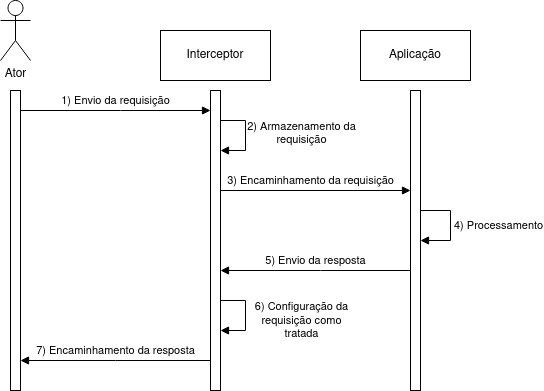
\includegraphics[scale=0.64]{images/interceptor-intercept.png}
\caption{Diagrama de sequência da interceptação de requisição pelo Interceptor.}
\label{fig:interceptor-request-interception}
\end{figure}

Agora para o fluxo de salvamento de uma imagem do contexto de estado da aplicação temos a
Figura \ref{fig:interceptor-checkpoint}. Neste fluxo, temos a comunicação do Interceptador
com o Administrador de Estado. A partir do momento em que o Interceptador percebe que é um
momento para salvamento, seja através de metadados sobre intervalos para coleta, como em \cite{vayghan2021kubernetes}, ou através de detecção de erro como em \cite{tran2022proactive},
ele inicia o fluxo. Inicialmente, todas as requisições param de ser encaminhadas à aplicação
e ficam apenas no \textit{buffer} do Interceptador, este, então, inicia o processo de salvamento
do estado da aplicação utilizando o CRIU. No momento que a imagem estiver pronta, os metadados
dela serão enviados ao Administrador de Estado, que contem principalmente a última requisição
servida, a identificação da aplicação e o horário da imagem. O Administrador de Estado internamente
irá salvar os metadados. Por fim, no Interceptador é retomado o processo de interceptação das
mensagens, servindo as mensagens no \textit{buffer} e reencaminhando novas que chegarem. Em \cite{muller2022architecture} teríamos um passo entre o 5 e o 6, que seria descartar as requisições no \textit{buffer} anteriores a este \textit{checkpoint}, não faremos esta abordagem, manteremos o \textit{buffer} com todas as requisições, salvando-as ou não em um banco de dados persistente, para
que possamos implementar nossa solução específica com técnicas de \textit{Event Sourcing} para
recuperação do estado da aplicação.

As requisições serão mantidas após um \textit{checkpoint}, como mostrado na Figura
\ref{fig:interceptor-checkpoint}, para que seja possível replicá-las a partir de 
ualquer imagem de recuperação ou até mesmo da última imagem possível. Através da
reprojeção das requisições como se fossem eventos, poderemos utilizar o padrão de
projeto de \textit{Event Sourcing} \cite{event-sourcing} para replicar o estado de uma
aplicação até o momento da falha apenas realizando todas as requisições novamente.
Isto poderá ser lento, mas, iremos utilizar esta técnica para comparar com a perda
de latência através de um \textit{checkpoint}, que precisa parar todas as requisições
momentaneamente.

\begin{figure}[h]
\centering
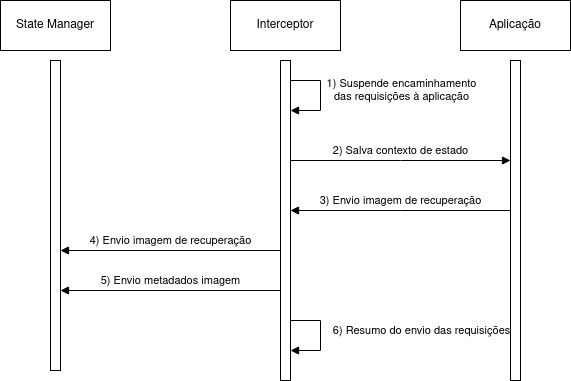
\includegraphics[scale=0.64]{images/interceptor-checkpoint.png}
\caption{Diagrama de sequência do salvamento de imagem feito pelo Interceptor.}
\label{fig:interceptor-checkpoint}
\end{figure}

Já para nossos Volumes para armazenamento persistente das imagens de recuperação
utilizamos os PersistenVolumes do Kubernetes, que possibilitam que os recursos
deste armazenamento persistente sejam acessíveis através de todo o \textit{cluster},
possibilitando que a imagem seja acessível em qualquer nó \cite{kubernetes:persistent-volumes}.
Já para o Banco de Dados utilizamos o etcd que já está presente no Kubernetes, que é
consistente e distribuído entre os nós do Kubernetes, ele permitirá salvar os metadados
das imagens e acessar através de qualquer réplica do State Manager \cite{etcd}
\cite{kubernetes:etcd}.

Por fim, temos o problema de interferir no tráfego da nossa aplicação a ser monitorada.
Conseguimos através da API do Kubernetes e do nosso Operator alterar um Service que iria
indicar o tráfego para o serviço e colocar nosso Interceptador para servir este Service,
pois eles funcionam por padrão como balanceadores de carga. Com isso temos a interceptação
através do Interceptador e podemos interromper as requisições à aplicação quando necessário.

\end{otherlanguage*}


    % Capítulo da implementação do Serviço.
    
% The \phantomsection command is needed to create a link to a place in the document that is not a
% figure, equation, table, section, subsection, chapter, etc.
% https://tex.stackexchange.com/questions/44088/when-do-i-need-to-invoke-phantomsection
\phantomsection

% Multiple-language document - babel - selectlanguage vs begin/end{otherlanguage}
% https://tex.stackexchange.com/questions/36526/multiple-language-document-babel-selectlanguage-vs-begin-endotherlanguage
\begin{otherlanguage*}{english}

% The \phantomsection command is needed to create a link to a place in the document that is not a
% figure, equation, table, section, subsection, chapter, etc.
% https://tex.stackexchange.com/questions/44088/when-do-i-need-to-invoke-phantomsection
\phantomsection

% Multiple-language document - babel - selectlanguage vs begin/end{otherlanguage}
% https://tex.stackexchange.com/questions/36526/multiple-language-document-babel-selectlanguage-vs-begin-endotherlanguage
\begin{otherlanguage*}{portuguese}

\chapter{\lang{Service Implementation}{Implementação do Serviço}} \label{cap:implementacao:servico}

Neste capítulo iremos trazer a experiência de implementação do Serviço para duas
diferentes implantações a primeira com CRIU e cri-o, que não conseguimos finalizar,
mas que possui importantes experiências e resolução de problemas a serem relatadas, e,
a segunda sendo a implantação utilizando técnicas de \textit{Event Sourcing} que foi
finalizada. Antes de apresentar as duas implementações iremos continuar apresentando
mais aplicações, bibliotecas e plataformas que utilizamos durante a implementação do
Serviço.

\section{Aplicações, bibliotecas e plataformas}

Para a implementação tanto do \textit{Checkpoint/Restore} com CRIU quanto com técnicas
de \textit{Event Sourcing} foi necessário a utilização de aplicações, bibliotecas e
plataformas que facilitaram o nosso desenvolvimento.

Um dos pontos iniciais para a implementação é o local para realizar a implantação do
Serviço. Inicialmente escolhemos utilizar a plataforma Emulab \cite{White+:osdi02}
que fornece máquinas virtuais sob demanda para computação distribuída. Embora, tudo
tenha funcionado bem com estas máquinas inicialmente, houveram dificuldades para
fazer funcionar o CRIU juntamente com o Kubernetes nas máquinas. Então, optamos por
trocar para outra solução mais comercial, o Google Cloud, nesta plataforma obtemos
uma máquina virtual permanente, desta forma, não era necessário refazer a configuração
da máquina todas as vezes. De modo, a economizar nos custos dos recursos de nossos testes,
eles foram feitos sob uma implantação em \textit{cluster} Kubernetes de máquinas com 2vCPU e 4GB
de memória, que é suficiente para executar um \textit{cluster} de nó único com Kubernetes.

Para possibilitar a existência da aplicação no Kubernetes nós precisamos adequar a
aplicação no fluxo de reconciliação de estado do Kubernetes através do conceito do Operador
\cite{kubernetes:operator}. Para isto, criamos três controladores, que são específicos para
cada recurso do Kubernetes e realizam o fluxo de reconciliação para os recursos, que juntos
implementam partes dos componentes da nossa arquitetura. O Interceptador é o único que não
foi implementado a através de um controlador. Teremos o controlador de Deployment, que é
responsável por verificar novos Deployments com anotação de monitoramento
\texttt{crsc.io/checkpoint-restore: true}, que indica que deve ser monitorado para
recuperação pelo Serviço, este controlador adiciona no Deployment o Interceptador como
um \textit{sidecar container}, que permitirá interceptar as requisições à aplicação alvo.
O controlador de Pod, será o responsável por monitorar os Pods e verificar quando houver a
anotação \texttt{crsc.io/checkpoint-restore: true} e o contêiner alvo da aplicação sofrer
uma falha, ou seja, não estiver no estado de Pronto do Kubernetes, ele ser agendado para
uma recuperação. Por fim, temos um outro controlador não totalmente
implementado, ele é o responsável por verificar o intervalo de \textit{Checkpoint} da
aplicação através da anotação do Deployment \texttt{crsc.io/checkpoint-interval}, sempre
que um novo Deployment monitorado for identificado, um recurso de Checkpoint é criado, e este
é monitorado pelo controlador do Checkpoint, quando se dá o momento do \textit{Checkpoint}
o controlador se comunica com o Interceptador e depois cria uma nova imagem a partir do
resultado do salvamento de estado do interceptador. Iremos cobrir com mais ênfase cada um
deles nas seções posteriores. Para construir todos este Operador, utilizamos o \textit{framework}
operator-sdk, que permite realizar a criação de recursos de Kubernetes e dos controladores
de maneira ágil e simples, abstraindo as intereções com o kube-apiserver e criação dos
Custom Resource Definition, que foram necessários para o novo recurso Checkpoint.

Ainda no contexto do \textit{Checkpoint}, como comentamos no capítulo de trabalhos
relacionados em \cite{schmidttransparent}, podemos obter um \textit{Checkpoint} da
aplicação utilizando o kubelet e as funcionalidades já implementadas para o cri-o
através da API do Kubernetes \cite{kubernetes:container-checkpoint}. Entretanto,
isso não nos gera uma imagem no formato do Open Container Initiative, devemos criar
essa imagem a partir de todos os passos que fizeram no trabalho em
\cite{schmidttransparent}. O caminho que optamos por seguir é um pouco diferente e
apresenta uma facilidade maior, na implementação de \cite{schmidttransparent} temos
o problema de dar manutenção na geração da imagem sempre que uma mudança na interface
ocorrer. Por isso, optamos por utilizar uma biblioteca e aplicação que já fizesse esta
parte a abstraisse o trabalho para nós, a biblioteca que encontramos, que também
funciona como uma aplicação de linha de comando, é o buildah\cite{buildah}. O buildah é
uma ferramenta especializada para facilitar a criação de imagens de contêineres no formato
do OCI.

Para armazenamento persistente dos dados da aplicação, como as requisições, utilizamos
o PostgreSQL \cite{postgresql} como banco de dados persistente. Ele será utilizado para
armazenar as requisições persistentemente quando necessário. Entretanto, a aplicação
pode funcionar utilizando memória, mas, esta implementação de memória existe problemas
dependendo da quantidade de memória livre para aplicação.

\section{Configuração do Cluster}

Para realizar a configuração do \textit{cluster} Kubernetes foram necessário realizar
algumas configurações e instalação de pacotes que fizessem CRIU, Kubernetes e buildah
funcionarem. Para configurar um \textit{cluster} Kubernetes com todas as funcionalidades
necessárias utilizamos Ubuntu 20.04, em máquinas com processador Intel Broadwell de
arquitetura x86/64 com 2vCPU e 4GB de memória, a partir disso precisamos executar a
sequência de comandos no Código \ref{listing:setup-script}, neste código utilizamos
o cri-o na versão 1.25, que é a versão mínima necessária para fornecer suporte à
funcionalidade de \textit{Container Checkpoint} utilizando CRIU no Kubernetes, que será
a funcionalidade utilizada na implementação com CRIU para prover salvamento do estado
da aplicação.

\begin{lstlisting}[language=bash,caption={Comandos de configuração da máquina para CRIU e cri-o.},label={listing:setup-script}]
   sudo sh -c 'echo "deb https://download.opensuse.org/repositories/devel:/kubic:/libcontainers:/stable/xUbuntu_20.04/ /" > /etc/apt/sources.list.d/devel:kubic:libcontainers:stable.list'
	sudo sh -c 'echo "deb http://download.opensuse.org/repositories/devel:/kubic:/libcontainers:/stable:/cri-o:/1.25/xUbuntu_20.04/ /" > /etc/apt/sources.list.d/devel:kubic:libcontainers:stable:cri-o:$CRIO_VERSION.list'
	curl -L https://download.opensuse.org/repositories/devel:/kubic:/libcontainers:/stable:/cri-o:/1.25/xUbuntu_20.04/Release.key | sudo apt-key add -
	curl -L https://download.opensuse.org/repositories/devel:/kubic:/libcontainers:/stable/xUbuntu_20.04/Release.key | sudo apt-key add -
	sudo apt-get update
	sudo apt-get install -y criu cri-o cri-o-runc
\end{lstlisting}

Primeiro adicionamos os repositórios para instalação do cri-o, que será utilizado como
\textit{runtime} de contêineres para o Kubernetes, e instalação dele, no mesmo comando
de instalação, instalamos o pacote do CRIU. No Código \ref{listing:setup-script} também
instalamos o \textit{backend} que o cri-o utiliza para contêineres, o runc, uma versão
específica deve ser instalada para que funcione o cri-o no Kubernetes.

Após instalado cri-o e CRIU, alteramos as configurações de ambos para que pudessemos
realizar o \textit{Checkpoint}. Primeiro, no Código \ref{listing:crio-conf}, alteramos
o comportamento da \textit{runtime} adicionando a opção que ativa o suporte para o CRIU
no cri-o e uma opção que remove a infraestrutura quando um contêiner não possui uma id de
processo privada, este deve ser ativado para mitigar um erro no cri-o. Estas alterações
foram feitas no arquivo /etc/crio/crio.conf.

\begin{lstlisting}[language=plaintext,caption={Configuração a ser incluída no arquivo de configurações do cri-o.},label={listing:crio-conf}]
[crio.runtime]
enable_criu_support = true # permite suporte a CRIU
drop_infra_ctr = false # remove a infra quando um pod não tem uma id de processo privada
\end{lstlisting}

Para que o CRIU possa utilizar o runc corretamente, também devemos editar a configuração
do CRIU. No Código \ref{listing:runc-conf}, editamos o arquivo /etc/criu/runc.conf para 
incluir configurações para fechar as conexões TCP no caso de uma restauração iniciada,
de modo que o cliente que iniciou a conexão TCP deverá refazê-la, para ignorar conexões
TCP já feitas no momento do \textit{Checkpoint}, onde o cliente também deverá refazer as
requisições, e desativamos a adiministração e cgroups feita pelo CRIU para utilizar o padrão,
para que seja possível executar o \textit{runc} no mesmo cgroup que cri-o e kubelet.

\begin{lstlisting}[language=plaintext,caption={Configuração a ser incluída no arquivo de configurações do runc para o CRIU.},label={listing:runc-conf}]
tcp-close # fecha as conexões TCP
skip-in-flight # ignora conexões já abertas que devem ser refeitas depois do checkpoint
manage-cgroups=ignore
\end{lstlisting}

A próxima parte requer que tenhamos buildah instalado e o componentes principais do nó
mestre do Kubernetes, o kubeadm e o kubelet, como também o kubectl para acessar o cluster
através da  API do Kubernetes. Os comandos para instalação destes pacotes e componentes podem
ser instalados através do Código \ref{listing:kubernetes-setup}. O comando \texttt{sudo apt-mark hold}
é necessário para que seja possível congelarmos a versão em utilização dos pacotes que especificamos,
neste caso os pacotes importantes para funcionamento do Kubernetes, que devem permanecer na mesma
versão para possibilitar o funcionamento correto do \textit{cluster}.

\begin{lstlisting}[language=bash,caption={Instalação dos pacotes necessários para Kubernetes e buildah.},label={listing:kubernetes-setup}]
sudo apt-get install -y apt-transport-https ca-certificates curl buildah make
sudo mkdir /etc/apt/keyrings
sudo sh -c "curl -fsSL https://pkgs.k8s.io/core:/stable:/v1.25/deb/Release.key | gpg --dearmor -o /etc/apt/keyrings/kubernetes-apt-keyring.gpg"
sudo sh -c 'echo "deb [signed-by=/etc/apt/keyrings/kubernetes-apt-keyring.gpg] https://pkgs.k8s.io/core:/stable:/v1.25/deb/ /" | tee /etc/apt/sources.list.d/kubernetes.list'
sudo apt-get update
sudo apt-get install -y kubelet kubeadm kubectl
sudo apt-mark hold kubelet kubeadm kubectl
\end{lstlisting}

Como o \text{Checkpoint} para contêineres no Kubernetes ainda é uma funcionalidade em alfa para
o Kubernetes, ela não é ativada automaticamente para toda nova instância de \textit{cluster}
Kubernetes. Precisamos alterar o funcionamento do Kubernetes para utilizar especificamente essa
funcionalidade, para isso existem os chamados \textit{Feature Gates} do Kubernetes que permitem
nas versões mais novas do Kubernetes ativar funcionalidades ainda não lançadas. Para ativar a
funcionalidade de \textit{Container Checkpoint} devemos alterar o arquivo de configuração que
determina a execução do kubelet no systemd do Ubuntu, em
/usr/lib/systemd/system/kubelet.service.d/10-kubeadm.conf, este arquivo deve estar como no
Código \ref{listing:kubelet-conf}. A parte que ativa o \textit{Feature Gate} é
\texttt{Environment="KUBELET\_FEATURE\_GATES\_ARGS=--feature-gates=ContainerCheckpoint=true"}. Já
a parte \texttt{Environment="KUBELET\_EXTRA\_ARGS=--cgroup-driver=systemd"} configura o kubelet
para utilizar o cgroup systemd para executar, isto coloca o cri-o no mesmo cgroup do kubelet, 
que permite que o último utilize o primeiro, caso isso não seja feito o kubelet não teria acesso
ao cri-o.

\begin{lstlisting}[language=plaintext,caption={Configuração do kubelet para executar no systemd com Feature Flag de ContainerCheckpoint e cgroup do systemd.},label={listing:kubelet-conf}]
[Service]
Environment="KUBELET_KUBECONFIG_ARGS=--bootstrap-kubeconfig=/etc/kubernetes/bootstrap-kubelet.conf --kubeconfig=/etc/kubernetes/kubelet.conf"
Environment="KUBELET_CONFIG_ARGS=--config=/var/lib/kubelet/config.yaml"
Environment="KUBELET_EXTRA_ARGS=--cgroup-driver=systemd"
Environment="KUBELET_FEATURE_GATES_ARGS=--feature-gates=ContainerCheckpoint=true"
# This is a file that "kubeadm init" and "kubeadm join" generates at runtime, populating the KUBELET_KUBEADM_ARGS variable dynamically
EnvironmentFile=-/var/lib/kubelet/kubeadm-flags.env
# This is a file that the user can use for overrides of the kubelet args as a last resort. Preferably, the user should use
# the .NodeRegistration.KubeletExtraArgs object in the configuration files instead. KUBELET_EXTRA_ARGS should be sourced from this file.
EnvironmentFile=-/etc/default/kubelet
ExecStart=
ExecStart=/usr/bin/kubelet $KUBELET_KUBECONFIG_ARGS $KUBELET_CONFIG_ARGS $KUBELET_KUBEADM_ARGS $KUBELET_EXTRA_ARGS $KUBELET_FEATURE_GATES_ARGS
\end{lstlisting}

Por fim, iniciamos o \textit{cluster} Kubernetes através dos comando no Código
\ref{listing:kubernetes-conf}, desativamos o swap da máquina para não criar conflitos que podem
ocorrer no kubelet. Outra seção do Código \ref{listing:kubernetes-conf} é a configuração do
KUBECONFIG, que é a configuração que o kubectl utiliza para se comunicar com a API do Kubernetes.
Ao final do código nós adicionamos um controlador de rede para os Pods do nosso sistema, qualquer
um pode ser utilizado, mas optamos por utilizar o Calico \cite{calico} pela facilidade em
instalação como vista na seção do Código \ref{listing:kubernetes-conf}.

\begin{lstlisting}[language=bash,caption={Inicialização do Kubernetes, configuração de acesso para o kubectl e instalação do administrador de rede para Pods Calico.},label={listing:kubernetes-conf}]
# Start Kubernetes

sudo swapoff -a
sudo kubeadm init --pod-network-cidr=192.168.0.0/16 --ignore-preflight-errors='all'

# Init kubectl

mkdir -p $HOME/.kube
sudo cp -i /etc/kubernetes/admin.conf $HOME/.kube/config
sudo chown $(id -u):$(id -g) $HOME/.kube/config

# Add network manager. We are going to install Calico.

kubectl create -f https://raw.githubusercontent.com/projectcalico/calico/v3.26.1/manifests/tigera-operator.yaml
kubectl create -f https://raw.githubusercontent.com/projectcalico/calico/v3.26.1/manifests/custom-resources.yaml
\end{lstlisting}

A partir das configurações listadas nesta seção obtivemos um \textit{cluster} Kubernetes funcional
pronto para iniciar nossas implementações, que permitem a utilização de CRIU para o \textit{Checkpoint}
e de buildah para construção das imagens de recuperação.

\section{Interceptador}

O nosso Interceptador como descrito nas seções anteriores é implantado a partir de um
\textit{sidecar container}, ambas as versões do Serviço, a de \textit{Checkpoint/Restore}
a partir do CRIU e a do \textit{Checkpoint/Restore} a partir de técnicas de
\textit{Event Sourcing} utilizam o mesmo Interceptador que é a funcionalidade comum aos
dois. Para criá-lo utilizamos a linguagem de programação Go e
realizamos uma construção de sua imagem utilizando Docker, não é necessário utilizar
cri-o para construir a imagem neste caso, pois as imagens geradas também seguem OCI.
A aplicação consiste de um servidor HTTP, este servidor possui algumas funcionalidades
expostas que serão chamadas de acordo com a necessidade dos outros componentes.
O Interceptador possui um estado interno que pode estar em dois valores diferentes,
ou em Ativo ou em Aguardo. No Ativo enviamos todas as requisições interceptadas a
aplicação alvo do Serviço, já no estado Aguardo nós realizamos o armazenamento das
requisições e esperamos o estado retornar a Ativo para continuar a entrega das
requisições. Enquanto seguimos o fluxo do diagrama da Figura
\ref{fig:interceptor-request-interception} para interceptação das requisições durante
o estado de Pronto do Interceptador, a Figura \ref{fig:diagram-wait-state-interceptor}
representa o fluxo de interceptação quando o estado do Interceptador é Aguardo.

\begin{figure}[h]
\centering
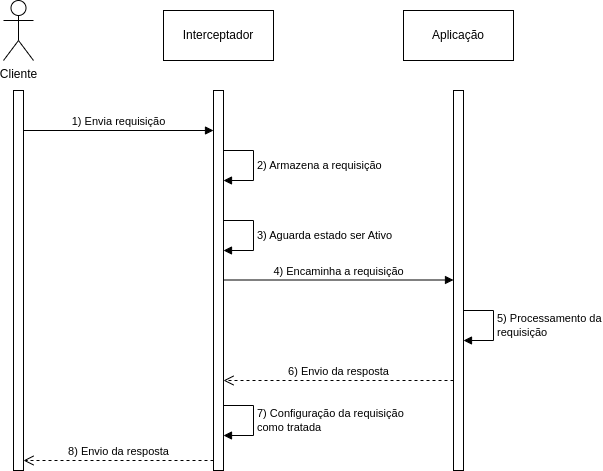
\includegraphics[scale=0.64]{images/wait-state.png}
\caption{Diagrama de sequência para tratamento de requisições durante estado de Aguardo do Interceptador.}
\label{fig:diagram-wait-state-interceptor}
\end{figure}

Para realizar um \textit{Checkpoint}, expomos uma rota HTTP de \texttt{/checkpoint}, que
chama a API do Kubernetes para que o kubelet comunique com o cri-o para realizar um 
\textit{Checkpoint} da aplicação executando no contêiner dentro do Pod alvo utilizando
CRIU. De modo a realizar a comunicação com o kube-apiserver precisamos estar autenticados
com o Kubernetes. Deste modo, criamos um Secret no Kubernetes, uma configuração de segredo
disponível na API do Kubernetes, com o certificado e key de assinatura para comunicação
com o kube-apiserver, estes arquivos ficam localizados no cluster em
\texttt{/etc/kubernetes/pki/apiserver-kubelet-client.key} e em
\texttt{/etc/kubernetes/pki/apiserver-kubelet-client.crt}, adicionamos estes dois arquivos em um
Secret como no Código \ref{listing:kubelet-secret}. Então, podemos chamarmos a API
do Kubernetes na rota \texttt{<https://ip-do-cluster/checkpoint/namespace/pod/container>}
utilizando o método HTTP POST, onde ip-do-cluster é o IP do \textit{cluster} Kubernetes,
é o \textit{namespace} do Kubernetes em que se encontra a aplicação do Kubernetes, pod é
o Pod que está executando a aplicação alvo e container o contêiner que está executando a
aplicação alvo. A partir daí, um \textit{Checkpoint} é salvo na máquina em
\texttt{/var/lib/kubelet/checkpoints} na forma de um arquivo compactado da forma
checkpoint-pod\_namespace-container-timestamp.tar, em que os valores são os mesmo,
exceto, \textit{timestamp}, que representa a string do momento em que o \textit{Checkpoint}
foi feito.

\begin{lstlisting}[language=bash,caption={Criação do Secret para comunicação com o kubelet para compartilhamento com nosso Interceptador.},label={listing:kubelet-secret}]
kubectl create secret generic kubelet-client-certs --from-file=client.crt=/etc/kubernetes/pki/apiserver-kubelet-client.crt --from-file=client.key=/etc/kubernetes/pki/apiserver-kubelet-client.key
\end{lstlisting}

Outra rota do Interceptador é a do estado em \texttt{/state}, através de uma chamada
HTTP ao método POST podemos alterar o estado com o parâmetro na \textit{query}
\texttt{state}, sendo ou Active, ou Waiting, que coloca o Interceptador nos estados,
respectivamente, de Ativou e Aguardo. O estado inicial do Interceptador é o Ativo.

Por fim, nós temos a rota \texttt{/reproject} que é a reprojeção de todas as requisições
interceptadas pelo Interceptador e aceita pela aplicação alvo. Esta reprojeção permite
que o estado seja alcançado. O ideal nesta reprojeção seria que ela pudesse ser feita a
partir de uma versão das requisições. Entretanto, não a fizemos porque não foi possível
finalizar a parte do \textit{Checkpoint/Restore} com CRIU que necessitaria desta parte.

\section{Checkpoint/Restore com CRIU}

Na implementação de \textit{Checkpoint/Restore} com CRIU criamos os três controladores do
nosso Operador, o controlador dos Deployments, o controlador dos Pods e o controlador do
nosso recurso customizado Checkpoint. Nesta implementação temos três passos para toda
aplicação monitorada, criação e implantação de um manifesto do Deployment da aplicação
no Kubernetes. Posterior criação do recurso customizado Checkpoint e monitoramento das
falhas do contêiner monitorado e posterior recuperação. Estes passos serão feitos pelos 
nossos controladores e descrevemos elas na próxima subseção.

\subsection{Controladores}

Todos os controladores do Kubernetes possuem um ciclo de reconciliação que deve
verificar o estado do \textit{cluster} e, em caso, de modificação do estado de algum
recurso que ele monitora deve agir de acordo com a alteração de estado para alcançar
um estado dos outros recursos de acordo com o que ele tem definido através dos manifestos
dos recursos.

\subsubsection{Controlador de Deployment}

O controlador do Deployment tem como seu recurso monitorado os Deployments do
\textit{cluster}. Sempre que uma aplicação é criada ela deve ser criada com anotações
no manifesto do Deploment, como \texttt{crsc.io/checkpoint-restore} e
\texttt{crsc.io/checkpoint-interval}, que são respectivamente, o valor booleano que
define se a aplicação é monitorada pelo Serviço ou não e o valor do intervalo de
\textit{Checkpoint} ativo. O diagrama da Figura \ref{fig:deployment-controller-diagram}
define o funcionamento do controlador.

\begin{figure}[h]
\centering
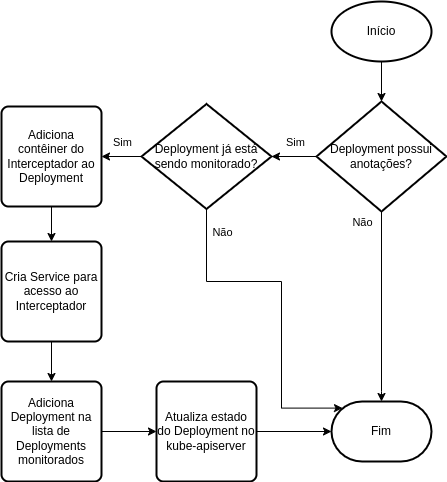
\includegraphics[scale=0.8]{images/deployment-controller.png}
\caption{Diagrama de fluxo para a injeção das configurações do Interceptador na aplicação alvo através de um Controlador de Deployments para o Operador.}
\label{fig:deployment-controller-diagram}
\end{figure}

A partir da alteração do estado do \textit{cluster} pela criação de um novo Deployment
monitorado o controlador realiza a criação de um novo recurso de Checkpoint. Este novo
recurso possui um manifesto com os valores de intervalo de \textit{Checkpoint} e também
as informações da aplicação monitorada, como o nome do Deployment. Este recurso será 
monitorado pelo controlador de Checkpoint que irá executar as ações necessárias para
alcançar o estado definido pelo manifesto.

Este controlador também deve injetar o Interceptador como um \textit{sidecar container}
ao Deployment da aplicação alvo. Sempre que um Deployment novo é adicionado com a 
anotação \texttt{crsc.io/checkpoint-restore} o manifesto do Deployment é alterado
para adicionar o contêiner do Interceptador como um \textit{sidecar container}, um novo
ReplicaSet é, então, criado pelo Kubernetes que criará um novo Pod com o nosso
Interceptador. Ao mesmo tempo o controlador cria um novo Service para o Interceptador no
novo Deployment que permite que o Interceptador seja acessado através de todo o cluster, o
Kubernetes lida com a parte do DNS e das configurações de rede.

Ao final temos a adição no manifesto do Deployment do conteúdo do contêiner como visto no
Código \ref{listing:sidecar-container}. Este contêiner tem montado na imagem um volume
que indica os arquivos de assinatura na comunicação com o kube-apiserver que criamos na
Seção de configuração do \textit{cluster}. Isto permite que o nosso Interceptador possa
se comunicar de forma segura e autenticada com o Kubernetes para solicitar um novo
\textit{Checkpoint} ao kubelet.

\begin{lstlisting}[language=yaml,caption={Configuração do Interceptador para o Deployment da aplicação alvo como sidecar container.},label={listing:sidecar-container}]
image: docker.io/gianaortiz/crsc-interceptor
imagePullPolicy: Always
name: interceptor
ports:
- containerPort: 8001
  hostPort: 8001
  protocol: TCP
resources: {}
terminationMessagePath: /dev/termination-log
terminationMessagePolicy: File
volumeMounts:
- mountPath: /var/run/secrets/kubelet-certs
  name: kubelet-certs
  readOnly: true
\end{lstlisting}

A partir desse momento nossa aplicação monitorada tem suas requisições interceptadas
pelo nosso Interceptador. Inicialmente, o estado é Ativo no Interceptador, então todas
as requisições serão primeiro armazenadas e depois encaminhadas à aplicação para que
elas sejam tratadas.

\subsubsection{Controlador de Pod}

Para implementar o nosso Administrador de Estado, implementamos parte dele no controlador
de Pod. O controlador tem uma adiministração mais passiva, através do ciclo de
reconciliação, quando um Pod apresenta um problema, como por exemplo, um dos contêineres
falhar, o controlador filtra os Pods que possuem a anotação
\texttt{crsc.io/checkpoint-restore}, adicionando a uma fila de restauração.
A restauração aconteceria a partir da configuração de utilização de uma nova
imagem à aplicação monitorada, entretanto, não conseguimos criar a imagem de
\textit{Checkpoint} e esta parte não foi feita.

Na Figura \ref{fig:restore-pod} temos o diagrama de como funciona esta parte. Primeiro o
controlador recebe uma atualização de estado dos Pods, verificando se o Pod é um Pod monitorado,
caso seja e tenha um contêiner com falha, ele será adicionado à fila de restauração. Caso a
atualização de estado indique que ele está pronto iremos buscar o Pod na fila de restauração,
então, a imagem da aplicação alvo será editada para que seja a imagem do último \textit{Checkpoint}
feito pelo controlador de Checkpoint. Após estabilização da imagem, colocamos o Interceptador no
estado Aguardo e é solicitado a ele a reprojeção ads requisições a partir da última requisição
recebida antes de se realizar o \textit{Checkpoint} atual. Ao final da reprojeção, o estado do
Interceptador é alterado para Ativo e as requisições são encaminhadas para a aplicação alvo
com o estado mais atual, fornecendo uma recuperação transparente ao usuário.

\begin{figure}[h!]
\centering
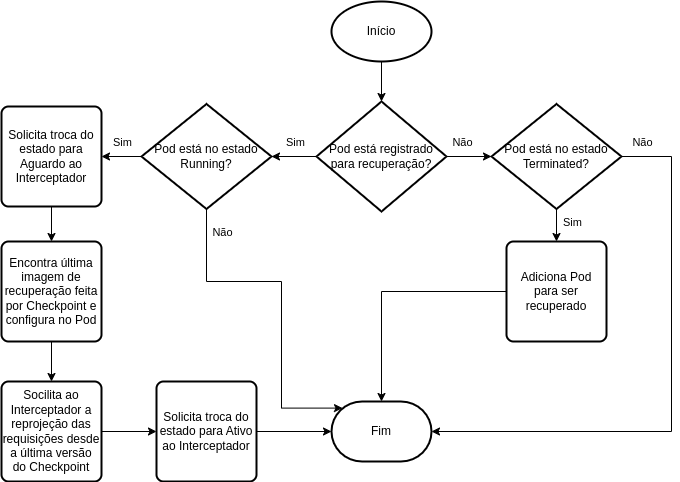
\includegraphics[scale=0.64]{images/restore-pod-criu.png}
\caption{Diagrama de fluxo para a recuperação da aplicação alvo através de um Controlador de Pods para o Operador com a implementação com CRIU.}
\label{fig:restore-pod}
\end{figure}

\subsubsection{Controlador de Checkpoint}

O controlador de Checkpoint realiza o ciclo de reconciliação para os recursos que nosso
Operador criou do tipo Checkpoint. O recurso Checkpoint possui o intervalo que é
passado através da anotação \texttt{crsc.io/checkpoint-interval} e o nome do Deployment
que está sendo monitorado. Através dessa anotação nosso controlador cria um processo que
será executado no intervalo dado para pedir um \textit{Checkpoint} ao Interceptador da
aplicação ao chamar a rota \texttt{/checkpoint} no Service do Interceptador. O Interceptador
irá pedir um novo \textit{Checkpoint} a API do kubelet e retornar sucesso. Após o sucesso,
este controlador irá obter esse \textit{Checkpoint} e criará uma imagem de contêiner no
formato OCI com buildah.

Como este controlador também implementa uma parte do nosso Administrador de Estado da 
arquitetura geral, ele também seria o responsável por salvar informações de metadados
sobre a imagem de salvamento criada. Entretanto, não foi possível criar uma aplicação
que conseguisse utilizar as bibliotecas do buildah para criação da imagem, muitos
problemas foram encontrados ao se utilizar overlayfs como comunicação de disco e não
houve tempo para realizar no nosso Serviço a geração da imagem. Porém, conseguimos criar
uma imagem com buildah através da sequência de comandos no Código
\ref{listing:buildah-build}, que podem ser refeitos através da biblioteca e agregados ao
Serviço.

\begin{lstlisting}[language=bash,caption={Comandos do buildah para construir a imagem de recuperação a partir de um Checkpoint feito pelo CRIU através do kubelet.},label={listing:buildah-build}]
newcontainer=$(buildah from scratch)
buildah add $newcontainer /var/lib/kubelet/checkpoints/checkpoint-<pod-name>_<namespace-name>-<container-name>-<timestamp>.tar /
buildah config --annotation=io.kubernetes.cri-o.annotations.checkpoint.name=<container-name> $newcontainer
buildah commit $newcontainer checkpoint-image:latest
buildah rm $newcontainer
\end{lstlisting}

Embora o \textit{Checkpoint} impeça as requisições de chegarem à aplicação alvo
diretamente, ele ocorre de forma transparente ao usuário da aplicação. O desenvolvedor
não necessita configurar nada na aplicação e não há percepção para o usuário que um
\textit{Checkpoint} está ocorrendo além de um possível aumento de latência como visto em
\cite{schmidttransparent}. Estes \textit{Checkpoints} periódicos seriam utilizados para
recuperar a aplicação ao último estado de forma mais rápida e eficiente como em
\cite{vayghan2021kubernetes} \cite{muller2022architecture} \cite{oh2018stateful} e
\cite{schmidttransparent}.

\section{Checkpoint/Restore com técnicas de Event Sourcing}

Na nossa implementação a partir de técnicas de Event Sourcing tinhamos o objetivo de
prover uma forma de agilizar a restauração da aplicação sem o problema do tempo que leva
para realizar o \textit{Checkpoint} da imagem. Já esperávamos que a performance para
aplicações com muitas requisições fosse pior, pois, necessitariamos reenviar todas as
requisições desde o início do estado de Pronto da aplicação. Mas, a partir dela
poderíamos unir com a técnica de \textit{Checkpoint} com CRIU para realizar ou uma ou
outra dependendo do estado atual do sistema, eliminando o tempo gasto em um
\textit{Checkpoint} no começo do estado de vida da aplicação. Assim, teremos algumas
modificações para alguns controladores que mostramos na Seção passada, já que alguns
passos não são realizados para nossa implementação com técnicas de \textit{Event Sourcing}.

\subsection{Controladores}

\subsubsection{Controlador de Deployment}

O controlador de Deployment para a implementação com técnicas de \textit{Event Sourcing} é
a mesma que para a implementação com CRIU, exceto, que, não criamos o recurso de Checkpoint neste
caso, pois, não há necessidade. Devido ao fato de sempre estarmos salvando as requisições
interceptados pelo Interceptador, sempre temos a ordem de requisições que precisamos
executar para obter o mesmo estado na aplicação alvo. Não precisamos realizar um
\textit{Checkpoint} periódico como no outro caso, pois, o salvamento de estado está nos
eventos que são gerados pelas requisições. Neste controlador, também adicionamos o 
\textit{sidecar container} ao Deployment e criamos o Service que redireciona requisições
ao Interceptador. O Interceptador tem sempre a mesma implementação, o que permite ser
utilizado em diferentes sistemas e diferentes contextos, já que tudo que ele provê é uma
API.

\subsubsection{Controlador de Pod}

O controlador de Pod para a implementação com técnicas de Event Sourcing funciona
diferente da implementação com CRIU. Pois, neste caso não precisamos alterar a imagem da
aplicação alvo, ela permanece a mesma sempre, tudo que precisamos realizar é a sequência
na Figura \ref{fig:pod-controller-event-sourcing}. Primeiro identificamos um contêiner
falhante a partir da atualização do kube-apiserver, adicionamos ele a uma fila de
restauração caso ele seja monitorado através das anotações. Posteriormente a isso, quando
o Pod atinge o estado de Pronto, recebemos mais uma atualização, caso o Pod esteja na
fila de recuperação o Interceptador será colocado no estado Aguardo, será solicitada a
reprojeção das requisições. Após o fim da reprojeção das requisições, que podem demorar,
já que devemos fazer todas desde o ínicio do funcionamento da aplicação alvo, alteramos
o estado do Interceptador para Pronto novamente. Novamente, de forma transparente
recuperamos o contêiner da aplicação alvo para um estado consistente.

\begin{figure}[h]
\centering
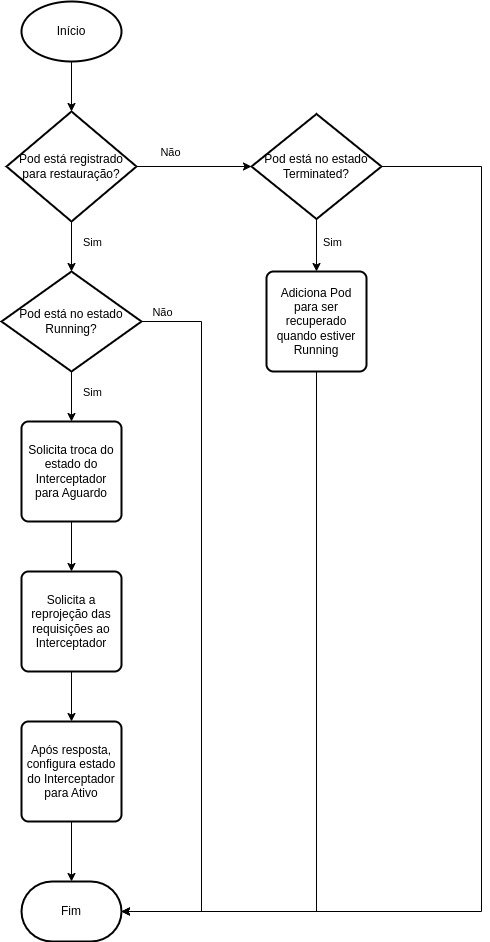
\includegraphics[scale=0.64]{images/restore-pod.png}
\caption{Diagrama de fluxo para a recuperação da aplicação alvo através de um Controlador de Pods para o Operador na implementação com técnicas de \textit{Event Sourcing}.}
\label{fig:pod-controller-event-sourcing}
\end{figure}

Desta forma, teriamos uma implementação que supostamente perderia performance dado
o número das requisições. Quanto mais requisições o sistema recebe, mais demorado seria
a reprojeção de todas as requisições, iremos validar este ponto na próxima Seção.
Entretanto, vale notar que esta é uma implementação não tão abordada em outros trabalhos,
exceto em \cite{muller2022architecture} que utiliza o conceito até certo ponto para
replicar as requisições a partir do último ponto de salvamento anterior a recuperação
da aplicação, o que diminui a latência em se recuperar a aplicação.

Como inicialmente pretendiamos adicionar as duas implementações, uma com CRIU e outra
com \textit{Event Sourcing}, pretendíamos aproveitar os pontos positivos de cada uma.
Entretanto, apenas a versão da implementação com técnicas de \textit{Event Sourcing}
foi finalizada e, pretendemos, na próxima Seção, investigar se essa implementação
realmente sofre de todas as partes negativas que apontamos nesta Seção.

\end{otherlanguage*}

    
    % Capítulo de avaliação experimental do Serviço.
    
% The \phantomsection command is needed to create a link to a place in the document that is not a
% figure, equation, table, section, subsection, chapter, etc.
% https://tex.stackexchange.com/questions/44088/when-do-i-need-to-invoke-phantomsection
\phantomsection

% Multiple-language document - babel - selectlanguage vs begin/end{otherlanguage}
% https://tex.stackexchange.com/questions/36526/multiple-language-document-babel-selectlanguage-vs-begin-endotherlanguage
\begin{otherlanguage*}{english}

% The \phantomsection command is needed to create a link to a place in the document that is not a
% figure, equation, table, section, subsection, chapter, etc.
% https://tex.stackexchange.com/questions/44088/when-do-i-need-to-invoke-phantomsection
\phantomsection

% Multiple-language document - babel - selectlanguage vs begin/end{otherlanguage}
% https://tex.stackexchange.com/questions/36526/multiple-language-document-babel-selectlanguage-vs-begin-endotherlanguage
\begin{otherlanguage*}{brazil}

\chapter{\lang{Experimental Analysis}{Análise Experimental}} \label{cap:analise:experimental}

Este capítulo apresenta a análise experimental sobre o Serviço criado. Para que seja possível
validar o Serviço uma aplicação de testes foi criada em Go, que é um acrescentador de valores
em memória. Sempre que uma requisição chega a ele, este incrementa um no seu valor em memória.
Esta é uma aplicação \textit{Stateful} e, portanto, é passível de ser utilizada no nosso Serviço.
Este capítulo pretende responder a algumas perguntas a partir da análise dos experimentos:

\begin{itemize}
	\item Existe impacto ao se utilizar o Interceptador para interceptar requisições à
	aplicação alvo? Este impacto deve ser considerado ao se utilizar o Serviço nas
	aplicações.
	\item Qual o impacto de tempo para a aplicação ser restaurada com a implementação do
	\textit{Checkpoint/Restore} com técnicas de \textit{Event Sourcing}?
	\item Qual o impacto geral na vazão e latência da aplicação quando ela está sendo
	interceptada pelo Interceptador? Qual a vazão e latência da aplicação quando ela
	está sendo executada \textit{standalone}? Há um impacto pela adição do Interceptador?
	\item Qual a latência da aplicação durante a recuperação da aplicação pelas técnicas de
	\textit{Event Sourcing}?
\end{itemize}

Para responder estas perguntas fizemos primeiro uma instrumentação no Serviço para que
pudessemos coletar pontos importante para análise, como, por exemplo, momentos em que a
aplicação alterou o estado do Interceptador, momento da introdução da falha do Interceptador,
momento da detecção pelo Administrador de Estado e tempo até a aplicação retornar ao estado
de Pronto. A análise de teste de carga para determinar a vazão e latência das requisições com
diferentes cargas no sistema. A partir disto pretendemos responder as perguntas para esta
análise. É importante destacar, que como a aplicação executa no mesmo nó, não há perdas
significativas de latência para comunicação entre serviços.

Para realizar o teste de carga, utilizamos a aplicação bombardier \cite{bombardier}, que
permite realizar um número arbitrário de requisições concorrentes, definindo a quantidade
de requisições e o tamanho da concorrência, que nos permite testar a aplicação sob uma
carga mais real. Para coleta de outras métricas utilizamos horário de início e fim de cada
uma das modificações. O Serviço e a aplicação executam na mesma máquina o horário é
igual para todos e não é necessário sincronização de relógios entre máquinas.

\section{Análise da inteterferência do Interceptador na aplicação}

Para fins de entender o quanto o Interceptador interfere no serviço que ele monitora,
instrumentamos a aplicação e utilizamos um teste de carga para verificar a performance
em três casos, da aplicação \textit{standalone}, isto é, sem a interferência do Interceptador,
da aplicação com o Interceptador utilizando memória para armazenamento das requisições e 
da aplicação com o Interceptador utilizando um banco de dados SQL para armazenamento das
requisições. Realizamos os mesmos testes de carga utilizando o bombardier para realizar
requisições com N clientes paralelamente durante dez segundos. A partir da finalização
das requisições obtivemos o valor de latência para o p95 da distribuição das requisições 
 pudemos construir um gŕafico de vazão por latência para os três casos, que é mostrado na Figura
\ref{fig:analysis-interceptor-standalone}.

O gŕafico da Figura \ref{fig:analysis-interceptor-standalone} nos provê informações que já
esperávamos, mas serão confirmadas por ele. Na aplicação \textit{standalone}, linha em vermelho,
podemos ver que demora muito para a aplicação atingir seu máximo de sobrecarga, somente entre
seis mil e dez mil clientes acabamos tendo uma performance que só piora a partir do aumento
da utilização do serviço. Inicialmente o serviço tem uma latência muito pequena, por exemplo,
com cinquenta clientes, temos apenas 5.11ms de latência.

A partir do momento que introduzimos o Interceptador temos uma piora, tanto da latência inicial,
quanto uma piora na questão da máxima vazão da aplicação. No caso da aplicação utilizando uma
implementação de armazenamento em memória, linha verde na Figura \ref{fig:analysis-interceptor-standalone},
temos que o máximo de carga do serviço se dá entre dois mil a dois mil e setecentos clientes
simultâneos. Há uma piora direta logo nos primeiros cinquenta clientes, onde a latência
p95 tem seu valor 38.55ms. Isto mostra que o impacto do nosso Interceptador e pelas
operações que ele faz, como, por exemplo, processamento da requisição obtendo apenas as
partes necessárias para o armazenamento, acréscimo da versão de ordem da requisição,
envio da requisição para a aplicação e posterior retorno da resposta para o cliente, geram
uma sobrecarga que influencia na performance do sistema como um todo. É importante notar que
a implementação em memória que utilizamos não tem possibilidade de realizar o \textit{Checkpoint},
já que não há memória infinita e não poderíamos armazenar todas as requisições em memória
que seriam necessárias para a reprojeção. Uma possibilidade de melhoria dessa abordagem,
que não foi feita, seria armazenar parte em memória e parte em um armazenamento fixo, como
um banco de dados ou em um arquivo.

Já na implementação do Interceptador com armazenamento em um banco de dados SQL, linha azul
na Figura \ref{fig:analysis-interceptor-standalone}, temos a pior performance de todas. Isto
se deve principalmente por dois fatores, da sobrecarga do sistema que realizamos os experimentos,
já que este estava executando o Kubernetes, um banco de dados, nosso Serviço e a aplicação
em uma máquina de 2vCPU e 4GB de memória, e também pela latência na inserção das entradas
de requisições no banco de dados. Como podemos ver na Figura \ref{fig:analysis-interceptor-standalone},
a capacidade máxima do sistema é atingida muito rapidamente, entre trezentos e quinhentos
clientes simultâneos. A aplicação também apresenta a pior performance em latência já no
começo dos experimentos com cinquenta clientes simultâneos, com uma latência de 151.94ms,
quase 400\% a mais que na implementação com o Interceptador com armazenamento em memória e
quase 3000\% a mais que na aplicação \textit{standalone}. Para utilizar essa solução em
um ambiente de produção seria necessário deixar a aplicação mais performática, através da
possibilidade de utilização de bancos mais rápidos, como de chave/valor ou de documentos.

\begin{figure}[h]
\centering
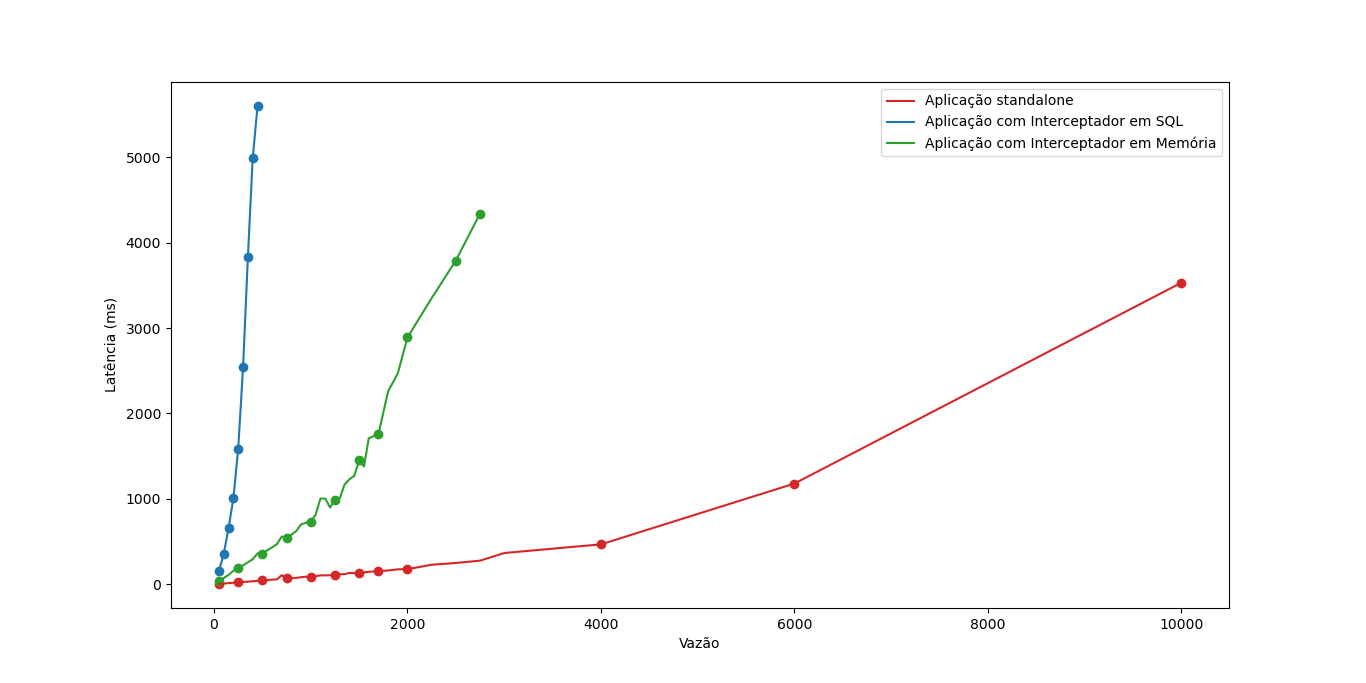
\includegraphics[scale=0.46]{images/vazaoxlatencia.png}
\caption{Gráfico de sobreposição de vazão X latência da aplicação alvo de forma \textit{standalone}, da aplicação alvo com o Interceptador com armazenamento em memória e da aplicação alvo com o Interceptador com armazenamento em banco de dados SQL.}
\label{fig:analysis-interceptor-standalone}
\end{figure}

Para nível de comparação no impacto do banco de dados na aplicação, instrumentamos o
código do Interceptador para capturar métricas sobre a latência em escrever a requisição
no banco de dados. Nas requisições com trezentos clientes simultâneos que obtemos uma
latência p95 de 1590ms, tivemos uma latência p95 para inserção da requisição no banco
de 1117ms, um impacto de cerca de 70.25\% na latência da aplicação. Uma estratégia seria combinar
a estratégia de implementação do armazenamento em memória com o armazenamento em banco de
dados SQL. Teríamos uma lista com tamanho fixo de dados, que armazenaria as requisições em
memória, onde a partir do momento em que ela excedesse sem máximo, iriamos escrever os dados no
banco de dados uma única vez, e continuariamos sobreescrevendo a lista. Com isto,
iríamos diminuir a latência de escrita, já que seria feita menos vezes e aumentar a
eficiência pelo armazenamento em memória.

\section{Análise do período de tempo de Checkpoint do Interceptador}

Nesta Seção, pretendemos discutir e analisar qual o tempo gasto pelo \textit{Checkpoint} do
Interceptador na implementação com CRIU. Na implementação com técnicas de
\textit{Event Sourcing} não temos uma alteração, por exemplo, da latência das requisições ao
se fazer um \textit{Checkpoint}, pois este ocorre passivamente. Já na implementação com CRIU
a aplicação deve ser pausada por um momento para salvamento do seu estado e isto gera uma
piora na qualidade de serviço para o usuário de maneira momentânea. Para simular este estado,
iniciamos realizando um teste de carga na aplicação para criar um estado, a partir daí, iniciamos
ao mesmo tempo um \textit{Checkpoint} a partir do Interceptador e um outro teste de carga, que deve
durar mais tempo que o \textit{Checkpoint}.

Coletamos dados para a latência das requisições que atingem o Interceptador em um período de
tempo que inclui antes de uma falha na aplicação alvo, durante a recuperação da aplicação
alvo e posteriormente da recuperação no mesmo teste. Estes testes nos proveram uma latência
p95 de 7.3s para as requisições do período de tempo, onde já existiam mil requisições
acumuladas para que ocorresse a reprojeção durante a recuperação e os tínhamos cem clientes
realizando mil requisições simultâneas para a aplicação durante o período de tempo.

Novamente, tivemos uma piora de latência do serviço, que se deve principalmente pelo fator
da nossa aplicação ter que realizar todas as requisições já feitas para a aplicação atingir
o estado antes da falha na recuperação. Na proposta de \cite{muller2022architecture} a
arquitetura realiza a poda das requisições, onde, menos requisições teriam que ser refeitas
a partir de uma falha para a recuperação através da criação de imagens de \textit{Checkpoint}
utilizando o CRIU.

\section{Análise da recuperação com técnicas de Event Sourcing}

Nesta Seção queremos investigar o impacto das técnicas de \textit{Event Sourcing} na
recuperação do estado de uma aplicação que falhou. Para isso, primeiro utilizamos nosso teste
de carga para levar a aplicação até um estado, com mil requisições(caso A), dez mil
requisições(caso B) e vinte mil requisições(caso C), com mais requisições acumuladas o serviço
degrada a ponto de não possibilitar testes com as configurações de \textit{cluster} que utilizamos.
Depois repetimos o mesmo teste com cada uma delas, ao alcançar o estado a aplicação terá uma falha
ocasionada pela interrupção da execução do container pela ferramenta crictl. Após a falha,
a recuperação deve ocorrer, neste momento, passamos a realizar um teste de carga igual para
todos os casos, cem requisições serão feitas de maneira concorrente entre dez clientes.

\begin{table}[htb]
\caption[Latência durante recuperação de requisições acumuladas.]{Latência durante recuperação de requisições acumuladas.}
\label{tab:event-sourcing-latency}
\centering
\begin{tabular}{|c|c|}
\hline
\textbf{\begin{tabular}[c]{@{}c@{}}Ńúmero de requisições\\ acumuladas\end{tabular}} & \textbf{Latência} \\ \hline
1000(A)                                                                            & 74.69ms             \\ \hline
10000(B)                                                                            & 122.76ms            \\ \hline
20000(C)                                                                               & 10010ms             \\ \hline
\end{tabular}
\end{table}

Os resultados do teste estão na Tabela \ref{tab:event-sourcing-latency}. Verificamos, que,
temos uma degradação relevante entre dez mil requisições acumuladas e vinte mil requisições
acumuladas, indo de 122.76ms de latência para 10010ms de latência para as requisições.
Novamente, quanto mais requisições acumuladas o Interceptador possui, mais demorada se torna
uma recuperação ao realizar todas as requisições novamente para a aplicação alvo. Esta análise
mostra uma premissa que já tínhamos, de que existe um limite para utilização das técnicas
de \textit{Event Sourcing} sobre o \textit{Checkpoint/Restore}, já que, conforme mais tempo
a aplicação vive, mais se torna necessário utilizar outras técnicas para ser possível reduzir
a replicação das requisições na recuperação, em \cite{muller2022architecture} a diminuição da
pilha foi feita através da implementação da recuperação com CRIU.

Agora, pretendemos também investigar o tempo que levamos entre a detecção, a recuperação e
atingir o estado de pronto em cada caso, como em \cite{vayghan2021kubernetes}, adicionamos
métricas ao controlador de Pods, para definir a detecção, e no nosso script identificamos o
início da falha, a recuperação é definida nos momentos em que se altera o estado do Interceptador
e o estado de Pronto também é instrumentado pelo controlador de Pods. Na Tabela
\ref{tab:latency-restoring} temos os valores para o início da recuperação após uma falha e o tempo
até a aplicação estar disponível novamente após a recuperação. No caso C temos um tempo muito
superior aos casos A e B, isto se deve por vários fatores, desde a configuração do nosso
\textit{cluster} que não permite escalabilidade e também da necessidade de se obter todas as
requisições de um banco de dados para replicação das requisições. A Tabela \ref{tab:latency-restoring}
demonstra que a implementação com técnicas de \textit{Event Sourcing} degrada conforme temos mais
requisições acumuladas no Interceptador para realizar a recuperação.

\begin{table}[htb]
\caption[Tempos de detecção de faha e de recuperação final de um contêiner alvo.]{Tempos de identificação de recuperação e de recuperação final de um contêiner alvo.}
\label{tab:latency-restoring}
\centering
\begin{tabular}{|c|c|c|}
\hline
\textbf{\begin{tabular}[c]{@{}c@{}}Ńúmero de requisições\\ acumuladas\end{tabular}} & \textbf{\begin{tabular}[c]{@{}c@{}}Tempo de detecção \\ (segundos) \end{tabular}} &
\textbf{\begin{tabular}[c]{@{}c@{}}Tempo de Recuperação \\ (segundos) \end{tabular}} \\ \hline
1000(A) &  0.991011s & 0.990702s \\ \hline
10000(B) & 0.998153s & 0.975395s     \\ \hline
20000(C) & 1.013021s & 856.67s \\ \hline
\end{tabular}
\end{table}

Na tabela \ref{tab:latency-restoring} percebemos que nosso limite da restauração quanto ao
número de requisições armazenadas está entre dez mil requisições e vinte mil requisições.
O aumento de cerca de 1s no tempo de restauração para cerca de 14min mostra uma perda de
performance muito grande. Seria essencial integrar outros \textit{Checkpoints} durante a
interceptação das requisições com o método de técnicas de \textit{Event Sourcing} para que
fosse possível diminuir o tempo de latência na recuperação a partir da dimunição da
quantidade de requisições armazenadas antes do último \textit{Checkpoint}.

\end{otherlanguage*}


    % Finaliza a parte no bookmark do PDF para que se inicie o bookmark na raiz
    % e adiciona espaço de parte no Sumário
    \phantompart

    % Capítulo de apresentação da conclusão, com trabalhos futuros, apresentando o que
    % falhamos na execução do trabalho.
    
% The \phantomsection command is needed to create a link to a place in the document that is not a
% figure, equation, table, section, subsection, chapter, etc.
% https://tex.stackexchange.com/questions/44088/when-do-i-need-to-invoke-phantomsection
\phantomsection

% ---
\chapter{\lang{Final Remarks}{Considerações Finais}} \label{cap:conclusion}
\phantomsection

	O trabalho desenvolvido nesse Trabalho de Conclusão de Curso, embora, não 
	tenha sido completamente finalizado, possibilitou uma análise sobre as técnicas
	de \textit{Checkpoint/Restore} para aplicações \textit{Stateful} no Kubernetes.
	Através da ferramenta CRIU, propusemos uma forma de implementar o
	\textit{Checkpoint/Restore}, que embora não tenha sido possível ser implementada
	no nosso Serviço, provou-se útil para realizar o salvamento do estado e posterior
	recuperação de uma aplicação. Já na implementação com técnicas de
	\textit{Event Sourcing} conseguimos realizar o Serviço de \textit{Checkpoint/Restore}
	no Kubernetes com transparência, provendo uma cópia utilizável da aplicação na
	tolerância a falhas a partir da reprojeção das requisições feitas a aplicação.
	
	O Serviço desenvolvido ainda possui algumas falhas, além de não conseguir
	implementar	o salvamento e recuperação com CRIU. Este só funciona com aplicações
	de estado que possuam uma réplica, mais réplicas geram estados incosistentes
	entre as aplicações. Também não houve muito foco na segurança do
	Serviço, já que temos acesso às chaves de comunicação com a API do Kubernetes
	em nosso Interceptador, qualquer um que tenha acesso ao Interceptador, por
	exemplo, através de uma exposição pela internet HTTP poderia obter acesso às
	chaves da API do Kubernetes e obter e alterar o estado do Kubernetes, expondo
	inclusive Secrets que devem funcionar como segredos no \textit{cluster}.

	A performance do nosso Serviço fica em evidência no Capítulo \ref{cap:analise:experimental},
	onde verificamos que a implementação necessita de melhorias na performance para
	que seja possível ser utilizada em aplicações em ambientes de produção. Como
	mostramos no capítulo existe uma evidência de que o armazenamento persistente
	através de um banco de dados SQL gera muita sobrecarga no sistema. Precisamos
	trabalhar em cima deste ponto, com modificações unindo implementação com
	armazenamento em memória e \textit{Checkpoint} com CRIU. Esta perda de
	performance já era esperada no início do trabalho.

	Por fim, o trabalho cumpriu com o seu objetivo, que era implementar um Serviço
	de \textit{Checkpoint/Restore} para aplicações \textit{Stateful} no Kubernetes.
	Conseguimos acoplar uma aplicação ao nosso Serviço a partir da utilização de
	anotações no Deployment, permitindo que o usuário do Serviço não tenha que
	realizar configurações na sua aplicação, realizar \textit{Checkpoints} passivos
	com técnicas de \textit{Event Sourcing} e restaurar a aplicação no caso de uma
	falha de forma transparente, onde a aplicação é restaurada para seu último estado
	de funcionamento. Também conseguimos entregar uma parte clara de como integrar o
	\textit{Checkpoint} com CRIU no nosso Serviço através da utilização do buildah
	para construção das imagens de recuperação.

\section{Trabalhos futuros}

Como trabalhos futuros podemos listar alguns pontos que faltaram fechar netes trabalho.
O primeiro é a implementação com CRIU para o \textit{Checkpoint/Restore}. Este trabalho
mostrou que é possível utilizar a arquitetura proposta para realizar o
\textit{Checkpoint/Restore}, mas não houve a finalização da implementação com CRIU,
porém listamos as partes e problemas que faltam para ser efetivada a implementação. Com
uma implementação com CRIU, podemos unir a implementação com técnicas de
\textit{Event Sourcing} para criar um serviço adaptativo que permita trocar o tipo de
restauração e definir o momento do início dos salvamentos de estado ativos através do
CRIU com base na análise da performance das duas implementações, seguindo os trabalhos
de \cite{muller2022architecture}, onde nossa arquitetura foi inspirada. 

Neste trabalho em momento algum utilizamos técnica preditivas para detectar o momento
que a aplicação poderia falhar, então, em determinados momentos poderiamos ter uma
requisição interceptada pelo Interceptador e que não tenha sido enviada à aplicação
com falhas. Em \cite{tran2022proactive} houve uma implementação de predição, que poderia
ser adicionada a nossa implementação para prover um Serviço mais ativo na recuperação,
que não espere a falha acontecer para agir.

Nosso trabalho não agiu com aplicações distribuídas geograficamente; Isto mostra uma
nova perspectiva, pois, será necessário espalhar os conteúdos tanto do Interceptador
quanto de imagens geradas para outros nós geograficamente distribuídos o que gera
latência de rede e tempo de restauração diferente dependendo da localização geográfica
do nó que falha. No trabalho de \cite{vayghan2021kubernetes}, tivemos uma análise da
distribuição geográfica e como poderíamos fazer para diminuir a latência através da
distribuição dos dados armazenados persistentemente.

O trabalho também não cobre aplicações que tenham mais de uma réplica com estado da
mesma aplicação. Neste Serviço cobrimos apenas aplicações com uma réplica.
Aplicações com diversas réplicas necessitam de coordenaçao entre os interceptadores
para acordar em uma ordem das requisições com algoritmos de consenso para resolver
estes problemas. Aliado ao problema de aplicações geograficamente distribuídas
também temos o consenso entre estas os diferentes nós geograficamente distribuídos.

Por fim, é possível aproveitar ainda mais de conceitos de \textit{Event Sourcing}.
A aplicação alvo se instrumentada também com este padrão de projeto pode prover uma
forma de obtermos o estado do sistema dela e salvarmos temporariamente no nosso
Serviço. Esta cópia pode ser o estado de cada objeto armazenado no sistema, no caso
de um banco de dados chave/valor, e a partir da finalização de uma requisição poderiamos
salvar esta cópia no Administrador de Estados e excluir requisições anteriores a ela,
reprojetando apenas as requisições a partir desta cópia.


    % ELEMENTOS PÓS-TEXTUAIS
    \postextual
    \setlength\beforechapskip{0pt}
    \setlength\midchapskip{15pt}
    \setlength\afterchapskip{15pt}

    % Referências bibliográficas
    \begingroup
        % https://tex.stackexchange.com/questions/163559/how-to-modify-line-spacing-per-entry-of-bibliography
        % https://tex.stackexchange.com/questions/19105/how-can-i-put-more-space-between-bibliography-entries-biblatex
        \setlength\bibitemsep{\baselineskip}
        \advisor{}{\linespread{1.18}\selectfont}

        % https://tex.stackexchange.com/questions/17128/using-bibtex-to-make-a-list-of-references-without-having-citations-in-the-body
        % \nocite{*}
        \printbibliography[title=\lang{REFERENCES}{REFERÊNCIAS}]
    \endgroup

    % Glossário, consulte o manual da classe abntex2 para orientações sobre o glossário.
    % \ifforcedinclude\else\glossary\fi

    % Inicia os apêndices
%    \begin{apendicesenv}
        % Imprime uma página indicando o início dos apêndices
%        \ifforcedinclude\else\partapendices\fi
%        \setlength\beforechapskip{50pt}
%        \setlength\midchapskip{20pt}
%        \setlength\afterchapskip{20pt}
%
%        


%
% How to fix the Underfull \vbox badness has occurred while \output is active on my memoir chapter style?
% https://tex.stackexchange.com/questions/387881/how-to-fix-the-underfull-vbox-badness-has-occurred-while-output-is-active-on-m
%

% ---

\lang
{\chapter[Page not filled]{Since this page is not being completely filled, it is generating the bottom bottom of the page}}
{\chapter[Página não gerada]{Como esta página não está sendo completamente preenchida, ele está gerando a caixa inferior inferior da página}}
% ---


% Multiple-language document - babel - selectlanguage vs begin/end{otherlanguage}
% https://tex.stackexchange.com/questions/36526/multiple-language-document-babel-selectlanguage-vs-begin-endotherlanguage
\begin{otherlanguage*}{english}

\showfont

1. How to display the font size in use in the final output,
2. How to display the font size in use in the final output,
3. How to display the font size in use in the final output,
4. How to display the font size in use in the final output,
5. How to display the font size in use in the final output,
6. How to display the font size in use in the final output,
7. How to display the font size in use in the final output,
8. How to display the font size in use in the final output,
9. How to display the font size in use in the final output,


% As this page is not being completely filled, it is generating the page bottom bad box.
% Fix Underfull \vbox (badness 10000) has occurred while \output is active
%
% \flushbottom vs \raggedbottom
% https://tex.stackexchange.com/questions/65355/flushbottom-vs-raggedbottom
\newpage



\section[Some encoding tests]{\showfont}

1. How to display the font size in use in the final output,
2. How to display the font size in use in the final output,
3. How to display the font size in use in the final output,
4. How to display the font size in use in the final output,
5. How to display the font size in use in the final output,
6. How to display the font size in use in the final output,

7. How to display the font size in use in the final output,
8. How to display the font size in use in the final output,
9. How to display the font size in use in the final output,
10. How to display the font size in use in the final output,
11. How to display the font size in use in the final output,
12. How to display the font size in use in the final output,

\subsection{\showfont}

1. How to display the font size in use in the final output,
2. How to display the font size in use in the final output,
3. How to display the font size in use in the final output,
4. How to display the font size in use in the final output,
5. How to display the font size in use in the final output,
6. How to display the font size in use in the final output,

7. How to display the font size in use in the final output,
8. How to display the font size in use in the final output,
9. How to display the font size in use in the final output,
10. How to display the font size in use in the final output,
11. How to display the font size in use in the final output,
12. How to display the font size in use in the final output,

\subsubsection{\showfont}

1. How to display the font size in use in the final output,
2. How to display the font size in use in the final output,
3. How to display the font size in use in the final output,
4. How to display the font size in use in the final output,
5. How to display the font size in use in the final output,
6. How to display the font size in use in the final output,

7. How to display the font size in use in the final output,
8. How to display the font size in use in the final output,
9. How to display the font size in use in the final output,
10. How to display the font size in use in the final output,
11. How to display the font size in use in the final output,
12. How to display the font size in use in the final output,

\subsubsubsection{\showfont}

1. How to display the font size in use in the final output,
2. How to display the font size in use in the final output,
3. How to display the font size in use in the final output,
4. How to display the font size in use in the final output,
5. How to display the font size in use in the final output,
6. How to display the font size in use in the final output,
7. How to display the font size in use in the final output,

8. How to display the font size in use in the final output,
9. How to display the font size in use in the final output,
10. How to display the font size in use in the final output,
11. How to display the font size in use in the final output,
12. How to display the font size in use in the final output,


Lipsum me [31-35]

\end{otherlanguage*}



%    \end{apendicesenv}

    % Inicia os anexos
   \begin{anexosenv}
       % Imprime uma página indicando o início dos anexos
       \ifforcedinclude\else\partanexos\fi
       \setlength\beforechapskip{50pt}
       \setlength\midchapskip{20pt}
       \setlength\afterchapskip{20pt}

       

%
% How to fix the Underfull \vbox badness has occurred while \output is active on my memoir chapter style?
% https://tex.stackexchange.com/questions/387881/how-to-fix-the-underfull-vbox-badness-has-occurred-while-output-is-active-on-m
%

% ----------------------------------------------------------
\chapter{\lang{Artigo}{Artigo}}
% ----------------------------------------------------------


Inclusão de um artigo científico no padrão da Sociedade Brasileira de Computação sobre o trabalho desenvolvido
no Trabalhao de Conclusão de Curso.

\modifiedincludepdf{-}{Artigo}{pictures/artigo.pdf}{0.9}



       


%
% How to fix the Underfull \vbox badness has occurred while \output is active on my memoir chapter style?
% https://tex.stackexchange.com/questions/387881/how-to-fix-the-underfull-vbox-badness-has-occurred-while-output-is-active-on-m
%

% ----------------------------------------------------------
\chapter{\lang{Código Fonte}{Código Fonte}}
% ----------------------------------------------------------

% Multiple-language document - babel - selectlanguage vs begin/end{otherlanguage}
% https://tex.stackexchange.com/questions/36526/multiple-language-document-babel-selectlanguage-vs-begin-endotherlanguage
\begin{otherlanguage*}{brazil}

O código fonte utilizado para elaboração deste Trabalho de Conclusão de Curso encontra-se disponível em
um repositório do Git acessível através do endereço https://github.com/GianOrtiz/checkpoint-restore-in-kubernetes.

\end{otherlanguage*}



   \end{anexosenv}

    % INDICE REMISSIVO
    \ifforcedinclude\else
        \phantompart
        \printindex
    \fi

\end{document}

